\part{Temporada Um}

\chapter{Aquele onde Tudo começou}

\textbf{RESUMO $\looparrowright$} Rachel foge do casamento e se encontra com os amigos na cafeteria. Ross está deprimido com seu divórcio, mas continua apaixonado por Rachel.

\begin{flushright}
\textcolor{gray600}{Exibido em Setembro, 21 1994}
\end{flushright}
\hypertarget{mr.-potato-head}{%
\section{Mr.~Potato Head}\label{mr.-potato-head}}

\begin{figure}[!ht]
  \begin{adjustwidth}{-\oddsidemargin-1in}{-\rightmargin}
    \centering
    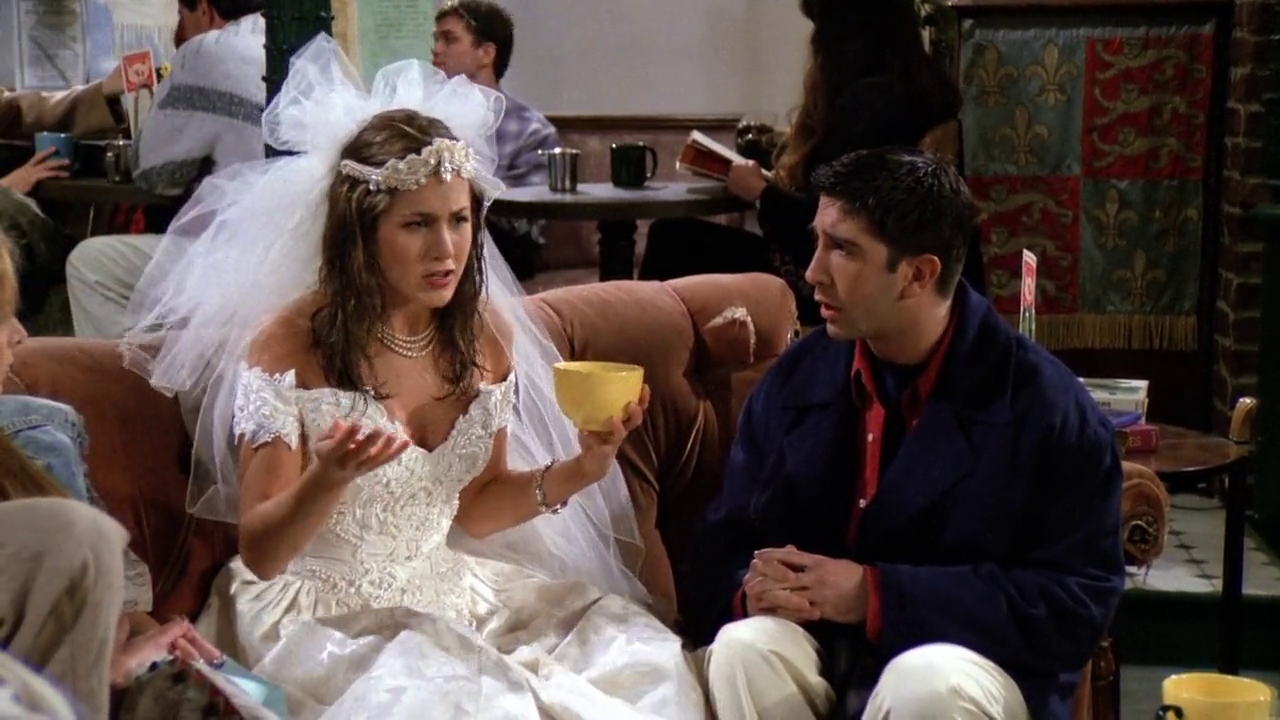
\includegraphics[trim={0 5cm 0 2cm,}, clip, width=\paperwidth]{./S01/img/1/mr-potato-head.png}
    \caption{Mr. Potato Head\label{fig:mr-potato-head}}
  \end{adjustwidth}
\end{figure}

\begin{tcolorbox}[enhanced,center upper,
    drop fuzzy shadow southeast, boxrule=0.3pt,
    lower separated=false,
    colframe=black!30!dialogoBorder,colback=white]
\begin{minipage}[c]{0.14\linewidth}
  \raisebox{\dimexpr-\height+\ht\strutbox\relax}{
    
\includegraphics[width=1.5cm]{./assets/img/rachel.png}
  }
   & \centering \scriptsize{Rachel}
\end{minipage}
\hspace{.1mm}
\begin{minipage}[c]{0.8\linewidth}
  \textbf{- [...] and that's when it hit me: How much Barry looks like Mr. Potato Head.}\\
  - [...] e me dei conta: O quanto Barry se parece com o Mr. Potato Head.
\end{minipage}
\end{tcolorbox}

\saveparinfos
\noindent
\begin{minipage}[c]{0.5\textwidth}\useparinfo

Rachel menciona que Barry, seu ex-noivo, parece com o \emph{Mr.~Potato
Head.} Trata-se de um brinquedo inventado por George Lerner, lançado
pela Hasbro em 1952. Em sua versão original havia apenas as partes, tais
como: os olhos, as orelhas e a boca, e era obrigação dos pais fornecerem
uma batata de verdade para formar a cabeça.

O \emph{Mr.~Potato Head} também pode ser visto nos filmes de \emph{Toy
Story} (1995, 1999, 2010, 2019), como um dos brinquedos do Andy.

\end{minipage}\hfill
\begin{minipage}[c]{0.45\textwidth}

\begin{figure}
  \centering
  \begin{tikzpicture}
    \node [inner sep=0pt] at (0,0) {
      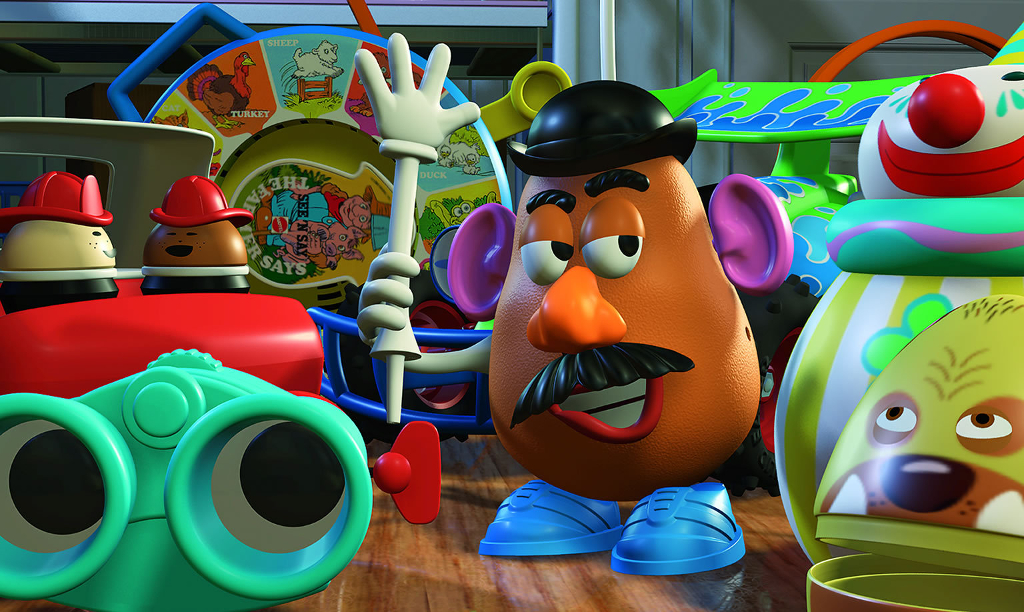
\includegraphics[width=0.8\textwidth,keepaspectratio]{./S01/img/1/mr-potato-head-toy-story.jpg}
    };
    \draw [white, rounded corners=\ClipSep, line width=\ClipSep]
    (current bounding box.north west) --
    (current bounding box.north east) --
    (current bounding box.south east) --
    (current bounding box.south west) -- cycle
    ;
    \end{tikzpicture}
    \caption{Mr. Potato Head (Toy Story)\label{fig:mr-potato-head-toy-story}}
\end{figure}

\end{minipage}

\hypertarget{referuxeancias}{%
\subsection{Referências}\label{referuxeancias}}

\begin{itemize}
\tightlist
\item
  \sloppy V&A Museum of Childhood. \url{https://www.vam.ac.uk/moc/collections/mr-potato-head/}
\item
  \sloppy Toy Story (IMDB). \url{https://www.imdb.com/title/tt0114709/}
\end{itemize}

\hypertarget{tres-destinos}{%
\section{Tres Destinos}\label{tres-destinos}}

\begin{figure}[!ht]
  \begin{adjustwidth}{-\oddsidemargin-1in}{-\rightmargin}
    \centering
    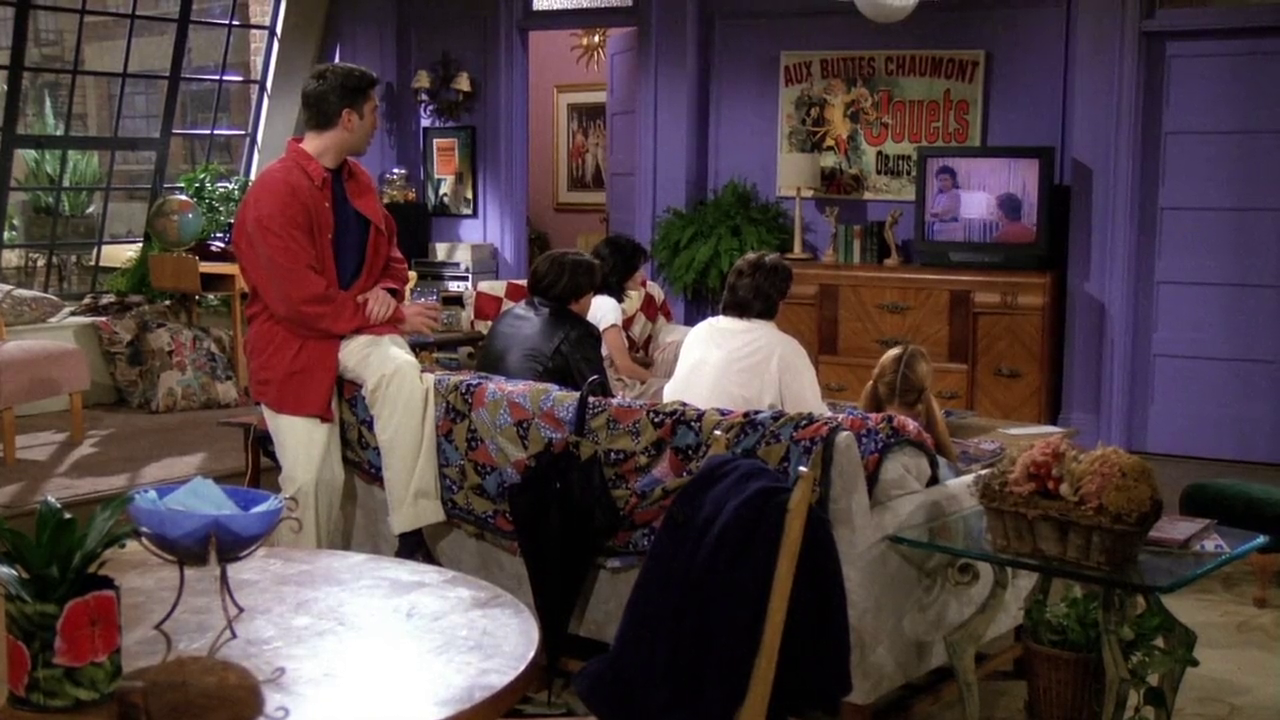
\includegraphics[trim={0 7cm 0 1.5cm,}, clip, width=\paperwidth]{./S01/img/1/tres-destinos.png}
    \caption{Tres Destinos\label{fig:tres-destinos}}
  \end{adjustwidth}
\end{figure}

Os amigos são vistos assistindo a telenovela \emph{Tres Destinos}
(1993), produzida para o mercado hispânico nos Estados Unidos. É a
clássica novela mexicana, do tipo popularmente exibida no Brasil, que
conta a história de 3 jovens irmãs unidas e separadas pelo mesmo homem,
com todos os ingredientes usuais: intriga, paixão, vingança, ódio,
ternura e amor.

\hypertarget{referuxeancias-1}{%
\subsection{Referências}\label{referuxeancias-1}}

\begin{itemize}
\tightlist
\item
  \sloppy EcuRed. \url{https://www.ecured.cu/Tres_destinos_(Telenovela)}
\item
  \sloppy IMDB. \url{https://www.imdb.com/title/tt0211876/}
\item
  \sloppy Abertura (YouTube). \url{https://www.youtube.com/watch?v=kfIk131FZxU}
\end{itemize}

\hypertarget{my-favorite-things}{%
\section{My Favorite Things}\label{my-favorite-things}}

\begin{figure}[!ht]
  \begin{adjustwidth}{-\oddsidemargin-1in}{-\rightmargin}
    \centering
    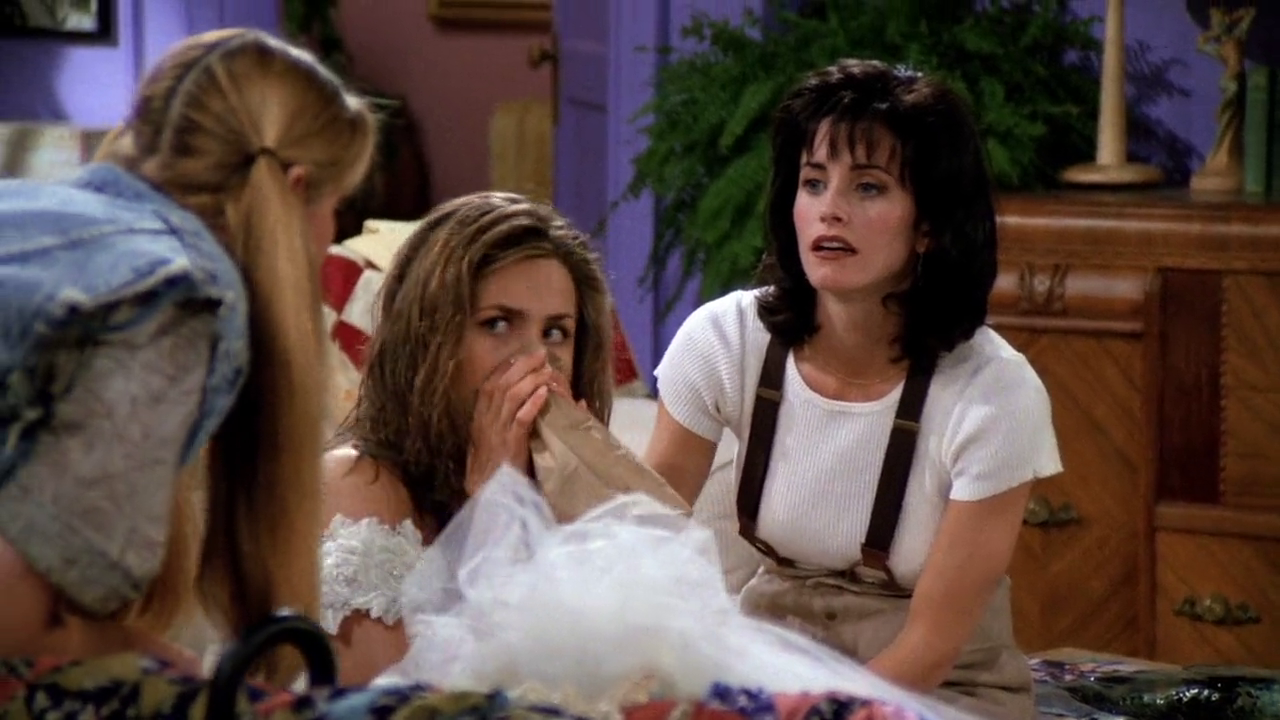
\includegraphics[trim={0 6cm 0 0.5cm,}, clip, width=\paperwidth]{./S01/img/1/my-favorite-things.png}
    \caption{My Favorite Things\label{fig:my-favorite-things}}
  \end{adjustwidth}
\end{figure}

Para acalmar Rachel, Phoebe canta uma versão própria da música \emph{My
Favorite Things} do musical \emph{The Sound of Music} (1959). Em 1965
foi lançado o filme, conhecido no Brasil como \emph{A Noviça Rebelde.}

A música expressa que você deve lembrar de suas coisas favoritas sempre
que se sentir triste.

\bigskip
\begin{tcolorbox}[enhanced,
    drop fuzzy shadow southeast, boxrule=0.3pt,
    lower separated=false, sidebyside, sidebyside align=top,
    halign=flush right, halign lower=left,
    colframe=black!30!dialogoBorder,colback=musicaBg]
\includegraphics[width=0.4cm]{./assets/img/icon-music.png}\\
When I’m feeling sad\\I simply remember my favorite things\\
\tcblower
\includegraphics[width=0.4cm]{./assets/img/icon-language.png}\\
Quando me sinto triste\\Simplesmente lembro de minhas coisas favoritas\\
\end{tcolorbox}

\begin{center}\rule{0.5\linewidth}{0.5pt}\end{center}

Versão da Phoebe:

\bigskip
\begin{tcolorbox}[enhanced,
    drop fuzzy shadow southeast, boxrule=0.3pt,
    lower separated=false, sidebyside, sidebyside align=top,
    halign=flush right, halign lower=left,
    colframe=black!30!dialogoBorder,colback=musicaBg]
\includegraphics[width=0.4cm]{./assets/img/icon-music.png}\\
Raindrops on roses\\And whiskers on kittens\\Doorbells and sleigh bells\\And something with mittens\\La la la la something with strings\\
\tcblower
\includegraphics[width=0.4cm]{./assets/img/icon-language.png}\\
Pingos de chuva em rosas\\E bigodes de gatinhos\\Campainhas e sinos\\E algo com luvas de lã\\La la la la algo com cordas\\
\end{tcolorbox}

Versão original:

\bigskip
\begin{tcolorbox}[enhanced,
    drop fuzzy shadow southeast, boxrule=0.3pt,
    lower separated=false, sidebyside, sidebyside align=top,
    halign=flush right, halign lower=left,
    colframe=black!30!dialogoBorder,colback=musicaBg]
\includegraphics[width=0.4cm]{./assets/img/icon-music.png}\\
Raindrops on roses\\And whiskers on kittens\\Bright copper kettles\\And warm woolen mittens\\Brown paper packages\\Tied up with strings\\
\tcblower
\includegraphics[width=0.4cm]{./assets/img/icon-language.png}\\
Pingos de chuva em rosas\\E bigodes de gatinhos\\Brilhantes tachos de cobre\\E quentes luvas de lã\\Pacotes de papel pardo\\Amarrado com cordas\\
\end{tcolorbox}

\begin{tcolorbox}[enhanced,center upper,
    drop fuzzy shadow southeast, boxrule=0.3pt,
    lower separated=false,
    colframe=black!30!dialogoBorder,colback=white]
\begin{minipage}[c]{0.14\linewidth}
  \raisebox{\dimexpr-\height+\ht\strutbox\relax}{
    
\includegraphics[width=1.5cm]{./assets/img/phoebe.png}
  }
   & \centering \scriptsize{Phoebe}
\end{minipage}
\hspace{.1mm}
\begin{minipage}[c]{0.8\linewidth}
  \textbf{- I helped.}\\
  - Eu ajudei.
\end{minipage}
\end{tcolorbox}

\hypertarget{referuxeancias-2}{%
\subsection{Referências}\label{referuxeancias-2}}

\begin{itemize}
\tightlist
\item
  \sloppy Trecho do filme The Sound of Music, em que é possível ouvir My Favorite Things (Youtube). \url{https://www.youtube.com/watch?v=DGABqdbtQnA}
\item
  \sloppy Wikipédia. \url{https://en.wikipedia.org/wiki/My_Favorite_Things_(song)}
\item
  \sloppy A Noviça Rebelde (IMDB). \url{https://www.imdb.com/title/tt0059742/}
\item
  \sloppy Letra e tradução - Vagalume. \url{https://www.vagalume.com.br/julie-andrews/my-favorite-things-traducao.html}
\end{itemize}

\hypertarget{maina-la-voyante}{%
\section{Maina La Voyante}\label{maina-la-voyante}}

\begin{figure}[!ht]
  \begin{adjustwidth}{-\oddsidemargin-1in}{-\rightmargin}
    \centering
    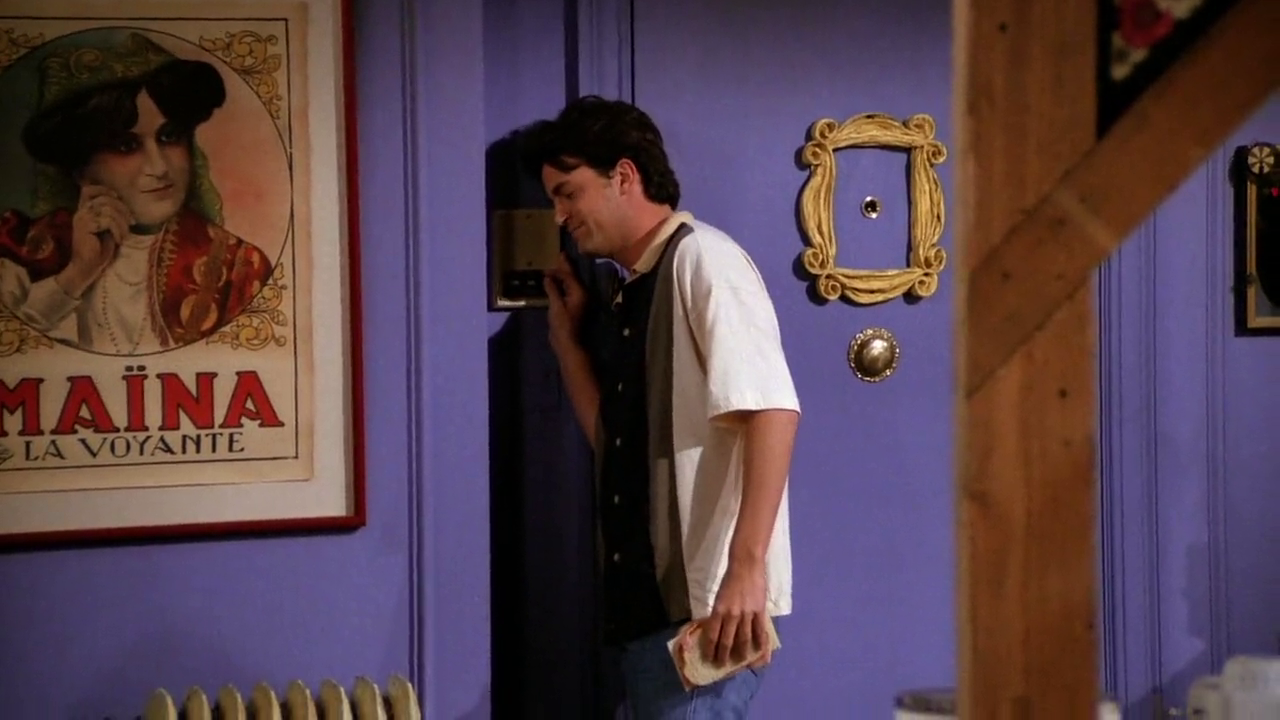
\includegraphics[trim={0 8cm 0 0.5cm,}, clip, width=\paperwidth]{./S01/img/1/maina-la-voyante.png}
    \caption{Maina La Voyante\label{fig:maina-la-voyante}}
  \end{adjustwidth}
\end{figure}

\saveparinfos
\noindent
\begin{minipage}[c]{0.5\textwidth}\useparinfo

Quando Chandler vai atender ao interfone, o poster \emph{Maina La
Voyante} pode ser visto, obra do ilustrador francês Louis Galice
(1864-1935).

\end{minipage}\hfill
\begin{minipage}[c]{0.6\textwidth}

\begin{figure}
  \centering
  \begin{tikzpicture}
    \node [inner sep=0pt] at (0,0) {
      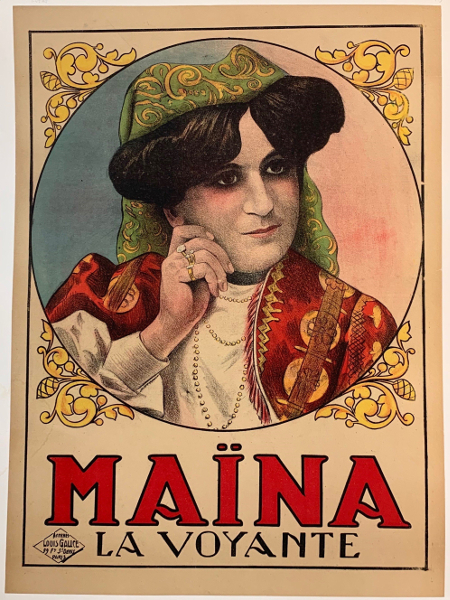
\includegraphics[width=0.6\textwidth,keepaspectratio]{./S01/img/1/maina-la-voyante-poster.jpg}
    };
    \draw [white, rounded corners=\ClipSep, line width=\ClipSep]
    (current bounding box.north west) --
    (current bounding box.north east) --
    (current bounding box.south east) --
    (current bounding box.south west) -- cycle
    ;
    \end{tikzpicture}
    \caption{Maina La Voyante - Poster\label{fig:maina-la-voyante-poster}}
\end{figure}

\end{minipage}

\hypertarget{referuxeancias-3}{%
\subsection{Referências}\label{referuxeancias-3}}

\begin{itemize}
\tightlist
\item
  \sloppy PosterMuseum. \url{https://postermuseum.com/products/maina-la-voyante}
\end{itemize}

\hypertarget{speed-racer}{%
\section{Speed Racer}\label{speed-racer}}

\begin{figure}[!ht]
  \begin{adjustwidth}{-\oddsidemargin-1in}{-\rightmargin}
    \centering
    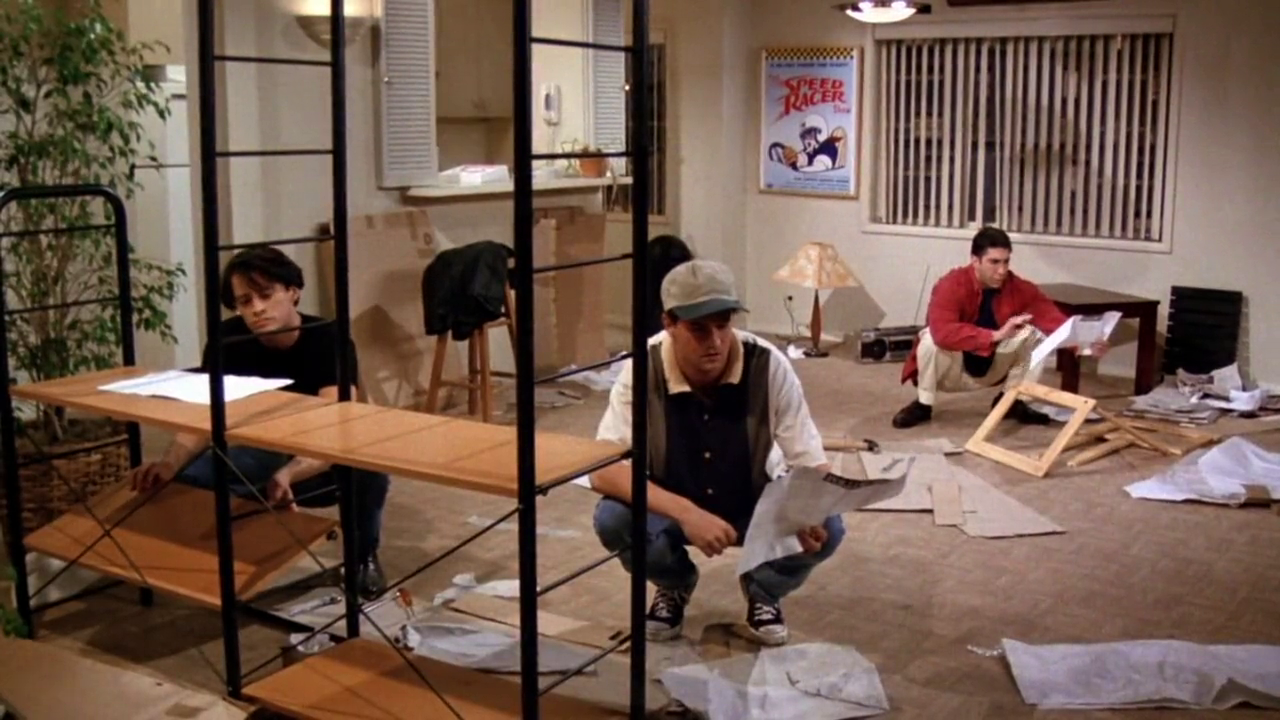
\includegraphics[trim={0 10cm 0 1cm,}, clip, width=\paperwidth]{./S01/img/1/speed-racer.png}
    \caption{Speed Racer\label{fig:speed-racer}}
  \end{adjustwidth}
\end{figure}

\saveparinfos
\noindent
\begin{minipage}[c]{0.5\textwidth}\useparinfo

No novo apartamento do Ross, é possível ver um poster de \emph{The Speed
Racer Show} (1967--1968) produzida pela \emph{Tatsunoko Production}.
Trata-se de uma série japonesa animada protagonizada por \emph{Go
Mifune}, conhecido como \emph{Speed Racer}. É baseada no mangá
\emph{Mach Go Go Go} (1966) criada por \emph{Tatsuo Yoshida}.

\end{minipage}\hfill
\begin{minipage}[c]{0.5\textwidth}

\begin{figure}
  \centering
  \begin{tikzpicture}
    \node [inner sep=0pt] at (0,0) {
      
\includegraphics[width=0.8\textwidth,keepaspectratio]{./S01/img/1/speed-racer-poster.jpeg}
    };
    \draw [white, rounded corners=\ClipSep, line width=\ClipSep]
    (current bounding box.north west) --
    (current bounding box.north east) --
    (current bounding box.south east) --
    (current bounding box.south west) -- cycle
    ;
    \end{tikzpicture}
    \caption{Speed Racer poster\label{fig:speed-racer-poster}}
\end{figure}

\end{minipage}

\hypertarget{referuxeancias-4}{%
\subsection{Referências}\label{referuxeancias-4}}

\begin{itemize}
\tightlist
\item
  \sloppy IMDB. \url{https://www.imdb.com/title/tt0061300/}
\item
  \sloppy Review do Omelete. \url{https://www.omelete.com.br/series-tv/lembra-desse-speed-racer-a-serie-original}
\item
  \sloppy Abertura (YouTube). \url{https://www.youtube.com/watch?v=suCm1w_KTiY}
\end{itemize}

\hypertarget{joanie-loves-chachi}{%
\section{Joanie Loves Chachi}\label{joanie-loves-chachi}}

\begin{figure}[!ht]
  \begin{adjustwidth}{-\oddsidemargin-1in}{-\rightmargin}
    \centering
    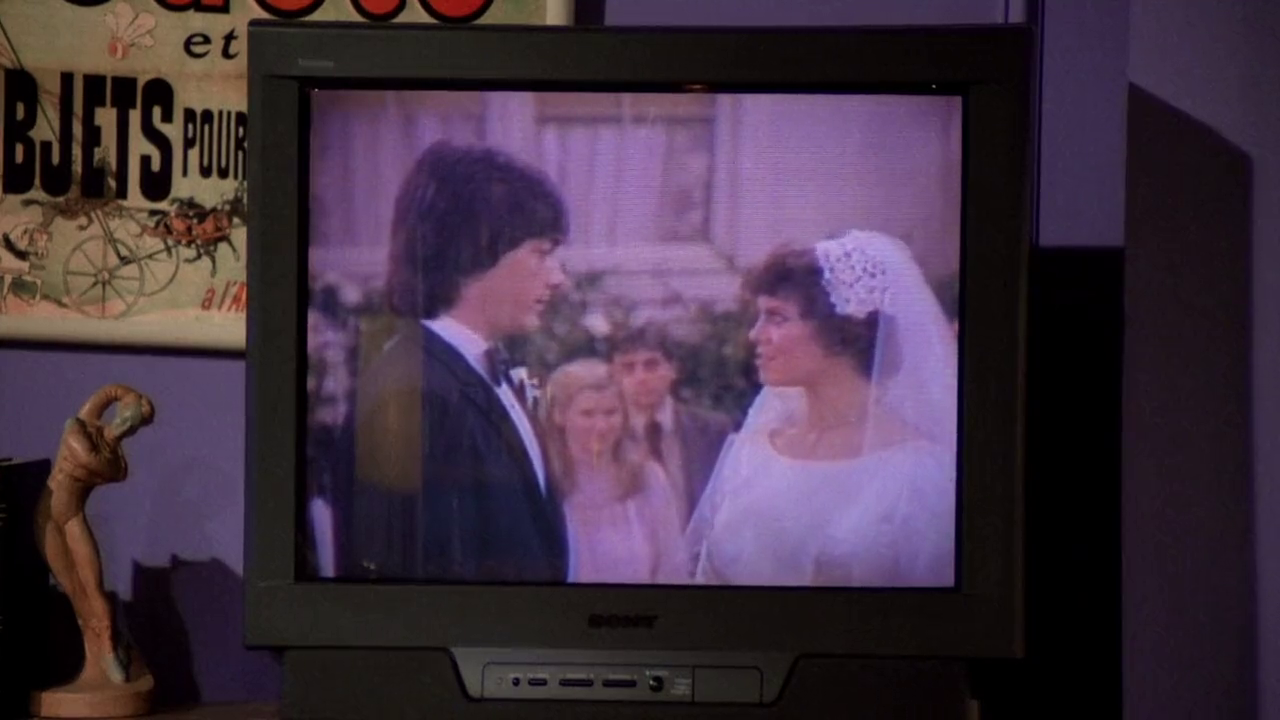
\includegraphics[trim={0 4cm 0 2cm,}, clip, width=\paperwidth]{./S01/img/1/joanie-loves-chachi.png}
    \caption{Joanie Loves Chachi\label{fig:joanie-loves-chachi}}
  \end{adjustwidth}
\end{figure}

\begin{tcolorbox}[enhanced,center upper,
    drop fuzzy shadow southeast, boxrule=0.3pt,
    lower separated=false,
    colframe=black!30!dialogoBorder,colback=white]
\begin{minipage}[c]{0.14\linewidth}
  \raisebox{\dimexpr-\height+\ht\strutbox\relax}{
    
\includegraphics[width=1.5cm]{./assets/img/rachel.png}
  }
   & \centering \scriptsize{Rachel}
\end{minipage}
\hspace{.1mm}
\begin{minipage}[c]{0.8\linewidth}
  \textbf{- But Joanie loved Chachi. That's the difference.}\\
  - Mas Joanie ama Chachi. Essa é a diferença.
\end{minipage}
\end{tcolorbox}

No apartamento de Monica, Rachel, ainda em seu vestido de noiva, assiste
a \emph{Joanie Loves Chachi} (1982--1983) - \emph{spin off} de
\emph{Happy Days} (1974) -, uma série de TV que mostra as aventuras
românticas de Joanie Cunningham e Chachi Arcola, buscando uma carreira
musical em Chicago.

\hypertarget{referuxeancias-5}{%
\subsection{Referências}\label{referuxeancias-5}}

\begin{itemize}
\tightlist
\item
  \sloppy IMDB. \url{https://www.imdb.com/title/tt0083433/}
\item
  \sloppy Wikipédia. \url{https://en.wikipedia.org/wiki/Joanie_Loves_Chachi}
\end{itemize}

\hypertarget{billy-dont-be-a-hero}{%
\section{Billy, don't be a hero}\label{billy-dont-be-a-hero}}

\begin{figure}[!ht]
  \begin{adjustwidth}{-\oddsidemargin-1in}{-\rightmargin}
    \centering
    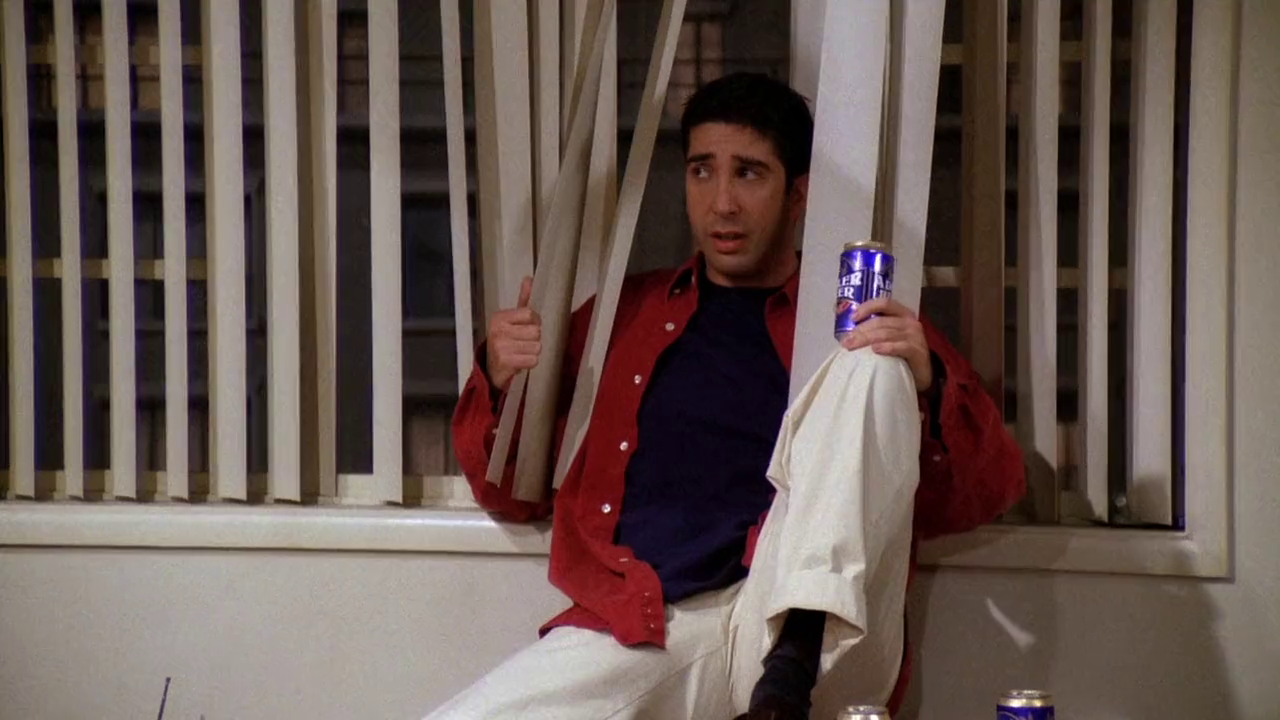
\includegraphics[trim={0 6.5cm 0 2.5cm,}, clip, width=\paperwidth]{./S01/img/1/billy-dont-be-a-hero.png}
    \caption{Billy, don’t be a hero\label{fig:billy-don-t-be-a-hero}}
  \end{adjustwidth}
\end{figure}

\begin{tcolorbox}[enhanced,center upper,
    drop fuzzy shadow southeast, boxrule=0.3pt,
    lower separated=false,
    colframe=black!30!dialogoBorder,colback=white]
\begin{minipage}[c]{0.14\linewidth}
  \raisebox{\dimexpr-\height+\ht\strutbox\relax}{
    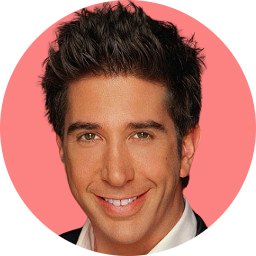
\includegraphics[width=1.5cm]{./assets/img/ross.png}
  }
   & \centering \scriptsize{Ross}
\end{minipage}
\hspace{.1mm}
\begin{minipage}[c]{0.8\linewidth}
  \textbf{- Do the words, 'Billy, don't be a hero', mean anything to you?}\\
  - As palavras, 'Billy, don't be a hero', significam alguma coisa pra vocês?
\end{minipage}
\end{tcolorbox}

\saveparinfos
\noindent
\begin{minipage}[c]{0.5\textwidth}\useparinfo

Ross faz menção a música \emph{Billy, don't be a hero} (1974) composta
por Mitch Murray e Peter Callander. Lançada inicialmente no Reino Unido
na voz de \emph{Paper Lace}, foi logo em seguida lançada também nos
Estados Unidos pelo grupo \emph{Bo Donaldson and The Heywoods.}

\end{minipage}\hfill
\begin{minipage}[c]{0.5\textwidth}

\begin{figure}
  \centering
  \begin{tikzpicture}
    \node [inner sep=0pt] at (0,0) {
      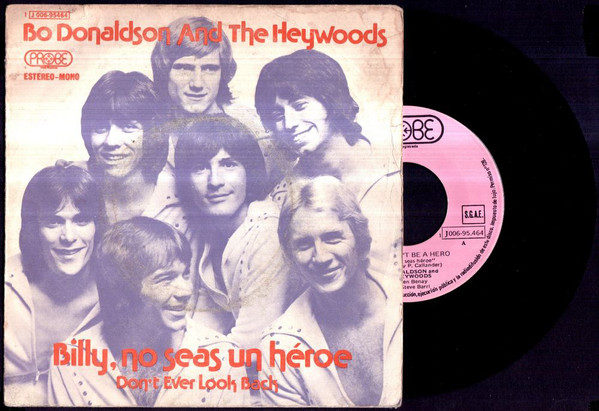
\includegraphics[width=0.8\textwidth,keepaspectratio]{./S01/img/1/billy-dont-be-a-hero-single.jpg}
    };
    \draw [white, rounded corners=\ClipSep, line width=\ClipSep]
    (current bounding box.north west) --
    (current bounding box.north east) --
    (current bounding box.south east) --
    (current bounding box.south west) -- cycle
    ;
    \end{tikzpicture}
    \caption{Billy, don’t be a hero - Single\label{fig:billy-don-t-be-a-hero-single}}
\end{figure}

\end{minipage}

\hypertarget{referuxeancias-6}{%
\subsection{Referências}\label{referuxeancias-6}}

\begin{itemize}
\tightlist
\item
  \sloppy Site Oficial. \url{http://www.bodonaldson.net/}
\item
  \sloppy IMDB. \url{https://en.wikipedia.org/wiki/Billy_Don%27t_Be_a_Hero}
\item
  \sloppy Letra - MetroLyrics. \url{https://www.metrolyrics.com/billy-dont-be-a-hero-lyrics-paper-lace.html}
\item
  \sloppy Billy, don’t be a hero - YouTube. \url{https://www.youtube.com/watch?v=1qlK9TJvuSk}
\end{itemize}

\hypertarget{pinocchio}{%
\section{Pinocchio}\label{pinocchio}}

\begin{figure}[!ht]
  \begin{adjustwidth}{-\oddsidemargin-1in}{-\rightmargin}
    \centering
    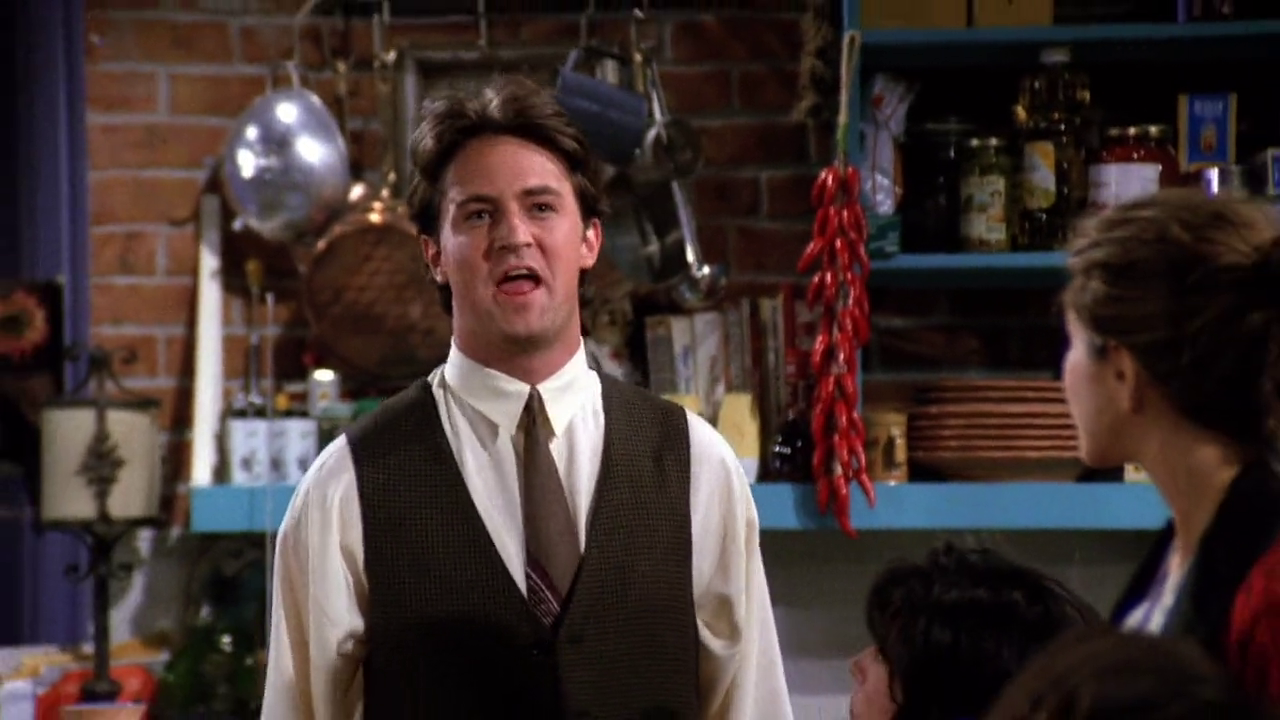
\includegraphics[trim={0 5cm 0 2cm,}, clip, width=\paperwidth]{./S01/img/1/pinocchio.png}
    \caption{Pinocchio\label{fig:pinocchio}}
  \end{adjustwidth}
\end{figure}

\begin{tcolorbox}[enhanced,center upper,
    drop fuzzy shadow southeast, boxrule=0.3pt,
    lower separated=false,
    colframe=black!30!dialogoBorder,colback=white]
\begin{minipage}[c]{0.14\linewidth}
  \raisebox{\dimexpr-\height+\ht\strutbox\relax}{
    
\includegraphics[width=1.5cm]{./assets/img/monica.png}
  }
   & \centering \scriptsize{Monica}
\end{minipage}
\hspace{.1mm}
\begin{minipage}[c]{0.8\linewidth}
  \textbf{- Wait, unless you happened to catch the Reruns' production of Pinocchio.}\\
  - Espera, a não ser que tenha visto a refilmagem do Pinóquio.
\end{minipage}

\medskip
\begin{minipage}[c]{0.14\linewidth}
  \raisebox{\dimexpr-\height+\ht\strutbox\relax}{
    
\includegraphics[width=1.5cm]{./assets/img/chandler.png}
  }
   & \centering \scriptsize{Chandler}
\end{minipage}
\hspace{.1mm}
\begin{minipage}[c]{0.8\linewidth}
  \textbf{- Look, Gepetto, I'm a real live boy.}\\
  - Olha, Gepetto, sou um menino de verdade.
\end{minipage}
\end{tcolorbox}

\saveparinfos
\noindent
\begin{minipage}[c]{0.5\textwidth}\useparinfo

Referência ao filme \emph{Pinocchio} (1940) ou \emph{Pinóquio} como
ficou conhecido no Brasil. Produzido pela \emph{Walt Disney}, o filme
conta a história de um velho carpinteiro chamado \emph{Gepetto}, que faz
um boneco de madeira chamado \emph{Pinóquio}, o qual é trazido a vida
pela \emph{Fada Azul}, com a condição de que ele demonstre obediência,
bravura e lealdade a seu criador.

\end{minipage}\hfill
\begin{minipage}[c]{0.5\textwidth}

\begin{figure}
  \centering
  \begin{tikzpicture}
    \node [inner sep=0pt] at (0,0) {
      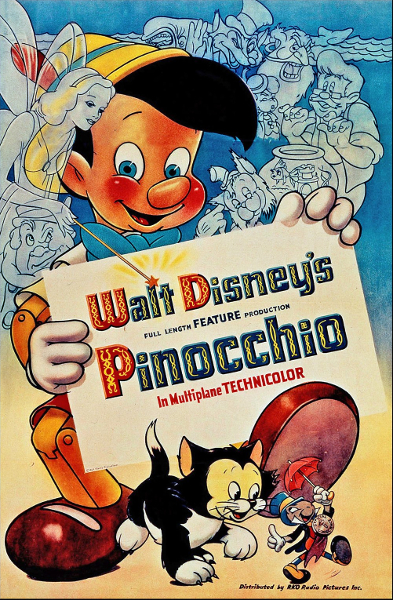
\includegraphics[width=0.5\textwidth,keepaspectratio]{./S01/img/1/pinocchio-poster.jpg}
    };
    \draw [white, rounded corners=\ClipSep, line width=\ClipSep]
    (current bounding box.north west) --
    (current bounding box.north east) --
    (current bounding box.south east) --
    (current bounding box.south west) -- cycle
    ;
    \end{tikzpicture}
    \caption{Pinocchio - Poster\label{fig:pinocchio-poster}}
\end{figure}

\end{minipage}

O filme tem muitos trechos musicais, e é daí que o Chandler retira
inspiração para a música que ele canta ao sair do apartamento:

\bigskip
\begin{tcolorbox}[enhanced,
    drop fuzzy shadow southeast, boxrule=0.3pt,
    lower separated=false, sidebyside, sidebyside align=top,
    halign=flush right, halign lower=left,
    colframe=black!30!dialogoBorder,colback=musicaBg]
\includegraphics[width=0.4cm]{./assets/img/icon-music.png}\\
Once I was a wooden boy,\\a little wooden boy…\\
\tcblower
\includegraphics[width=0.4cm]{./assets/img/icon-language.png}\\
Uma vez eu era um garoto de madeira,\\Um pequeno garoto de madeira…\\
\end{tcolorbox}

\hypertarget{referuxeancias-7}{%
\subsection{Referências}\label{referuxeancias-7}}

\begin{itemize}
\tightlist
\item
  \sloppy IMDB. \url{https://www.imdb.com/title/tt0032910/}
\item
  \sloppy Wikipédia. \url{https://pt.wikipedia.org/wiki/Pin%C3%B3quio_(filme)}
\end{itemize}

\hypertarget{liza-minnelli}{%
\section{Liza Minnelli}\label{liza-minnelli}}

\begin{figure}[!ht]
  \begin{adjustwidth}{-\oddsidemargin-1in}{-\rightmargin}
    \centering
    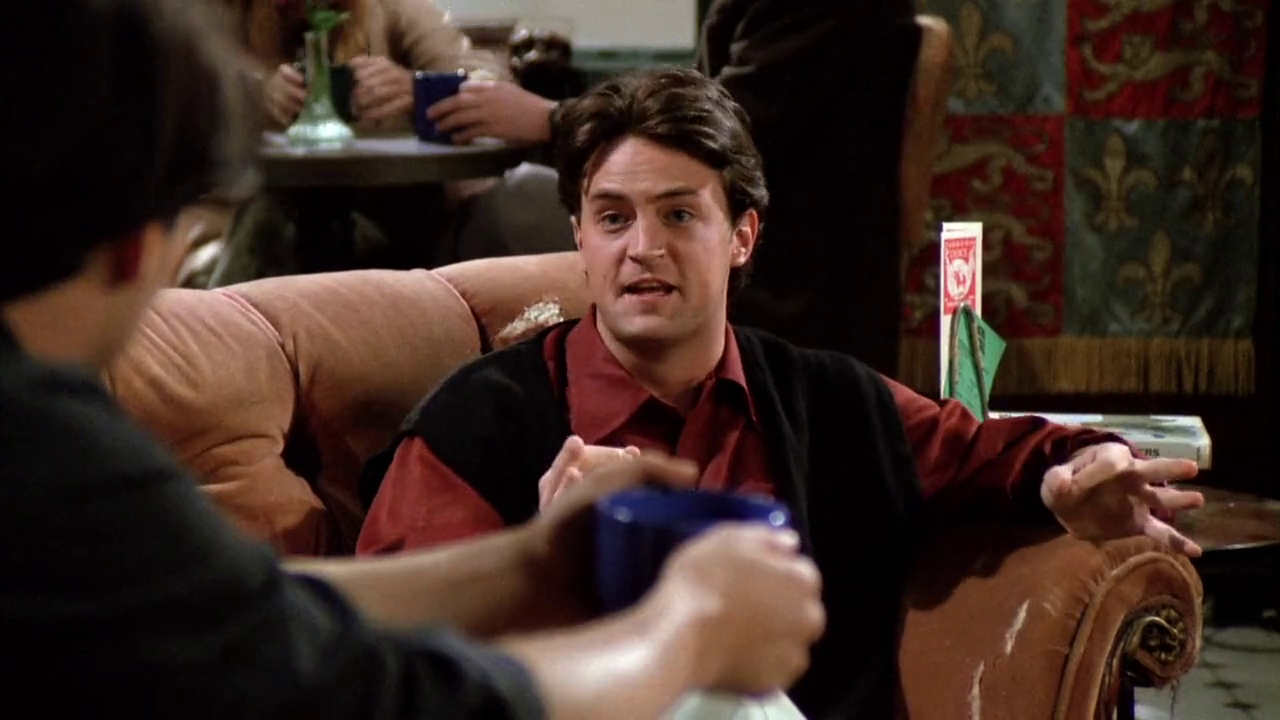
\includegraphics[trim={0 5cm 0 2cm,}, clip, width=\paperwidth]{./S01/img/1/liza-minnelli.png}
    \caption{Liza Minnelli\label{fig:liza-minnelli}}
  \end{adjustwidth}
\end{figure}

\begin{tcolorbox}[enhanced,center upper,
    drop fuzzy shadow southeast, boxrule=0.3pt,
    lower separated=false,
    colframe=black!30!dialogoBorder,colback=white]
\begin{minipage}[c]{0.14\linewidth}
  \raisebox{\dimexpr-\height+\ht\strutbox\relax}{
    
\includegraphics[width=1.5cm]{./assets/img/chandler.png}
  }
   & \centering \scriptsize{Chandler}
\end{minipage}
\hspace{.1mm}
\begin{minipage}[c]{0.8\linewidth}
  \textbf{- Kids, new dream. I'm in Las Vegas. I'm Liza Minnelli.}\\
  - Crianças, novo sonho. Tô em Las Vegas. Eu sou Liza Minelli.
\end{minipage}
\end{tcolorbox}

\saveparinfos
\noindent
\begin{minipage}[c]{0.5\textwidth}\useparinfo

Chandler menciona a atriz e cantora americana \emph{Liza Minnelli}
(1946-), é conhecida por ganhar o Oscar de melhor atriz por sua atuação
no filme \emph{Cabaret} (1972).

\end{minipage}\hfill
\begin{minipage}[c]{0.5\textwidth}

\begin{figure}
  \centering
  \begin{tikzpicture}
    \node [inner sep=0pt] at (0,0) {
      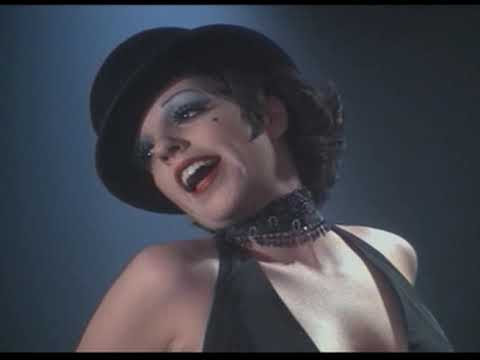
\includegraphics[width=0.8\textwidth,keepaspectratio]{./S01/img/1/liza-minnelli-cabaret.jpg}
    };
    \draw [white, rounded corners=\ClipSep, line width=\ClipSep]
    (current bounding box.north west) --
    (current bounding box.north east) --
    (current bounding box.south east) --
    (current bounding box.south west) -- cycle
    ;
    \end{tikzpicture}
    \caption{Liza Minnelli - Cabaret\label{fig:liza-minnelli-cabaret}}
\end{figure}

\end{minipage}

\hypertarget{referuxeancias-8}{%
\subsection{Referências}\label{referuxeancias-8}}

\begin{itemize}
\tightlist
\item
  \sloppy IDMB. \url{https://www.imdb.com/name/nm0591485/}
\item
  \sloppy Wikipédia. \url{https://pt.wikipedia.org/wiki/Liza_Minnelli}
\end{itemize}


\chapter{Aquele com o Ultrassom no Final}

\textbf{RESUMO $\looparrowright$} A ex-mulher de Ross está grávida dele, mas ele não gosta do sobrenome que ela escolheu para o bebê.

\begin{flushright}
\textcolor{gray600}{Exibido em Setembro, 28 1994}
\end{flushright}
\hypertarget{pink-floyd}{%
\section{Pink Floyd}\label{pink-floyd}}

\begin{figure}[!ht]
  \begin{adjustwidth}{-\oddsidemargin-1in}{-\rightmargin}
    \centering
    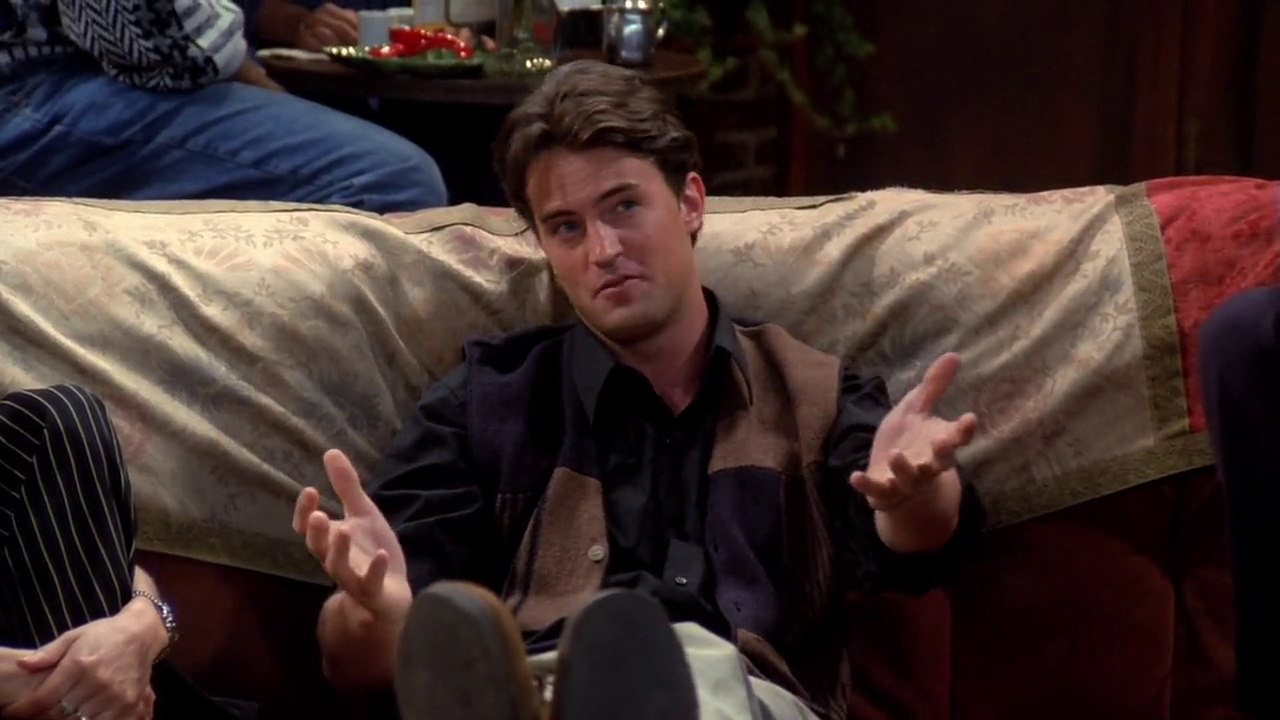
\includegraphics[trim={0 5cm 0 2cm,}, clip, width=\paperwidth]{./S01/img/2/pink-floyd.png}
    \caption{Pink Floyd\label{fig:pink-floyd}}
  \end{adjustwidth}
\end{figure}

\begin{tcolorbox}[enhanced,center upper,
    drop fuzzy shadow southeast, boxrule=0.3pt,
    lower separated=false,
    colframe=black!30!dialogoBorder,colback=white]
\begin{minipage}[c]{0.14\linewidth}
  \raisebox{\dimexpr-\height+\ht\strutbox\relax}{
    
\includegraphics[width=1.5cm]{./assets/img/chandler.png}
  }
   & \centering \scriptsize{Chandler}
\end{minipage}
\hspace{.1mm}
\begin{minipage}[c]{0.8\linewidth}
  \textbf{- ...before Pink Floyd comes out.}\\
  - ...antes do show do Pink Floyd.
\end{minipage}
\end{tcolorbox}

Chandler menciona a banda britânica de rock progressivo \emph{Pink
Floyd}, formada em 1965. A banda lança o albúm \emph{The Division Bell}
em Março 1994, um pouco antes do começo da série.

\begin{figure}
  \centering
  \begin{tikzpicture}
    \node [inner sep=0pt] at (0,0) {
      
\includegraphics[width=0.5\textwidth,keepaspectratio]{./S01/img/2/the-division-bell.jpg}
    };
    \draw [white, rounded corners=\ClipSep, line width=\ClipSep]
    (current bounding box.north west) --
    (current bounding box.north east) --
    (current bounding box.south east) --
    (current bounding box.south west) -- cycle
    ;
    \end{tikzpicture}
    \caption{The Division Bell\label{fig:the-division-bell}}
\end{figure}

\hypertarget{referuxeancias}{%
\subsection{Referências}\label{referuxeancias}}

\begin{itemize}
\tightlist
\item
  \sloppy Site oficial. \url{https://www.pinkfloyd.com/}
\end{itemize}

\hypertarget{threes-company}{%
\section{Three's Company}\label{threes-company}}

\begin{figure}[!ht]
  \begin{adjustwidth}{-\oddsidemargin-1in}{-\rightmargin}
    \centering
    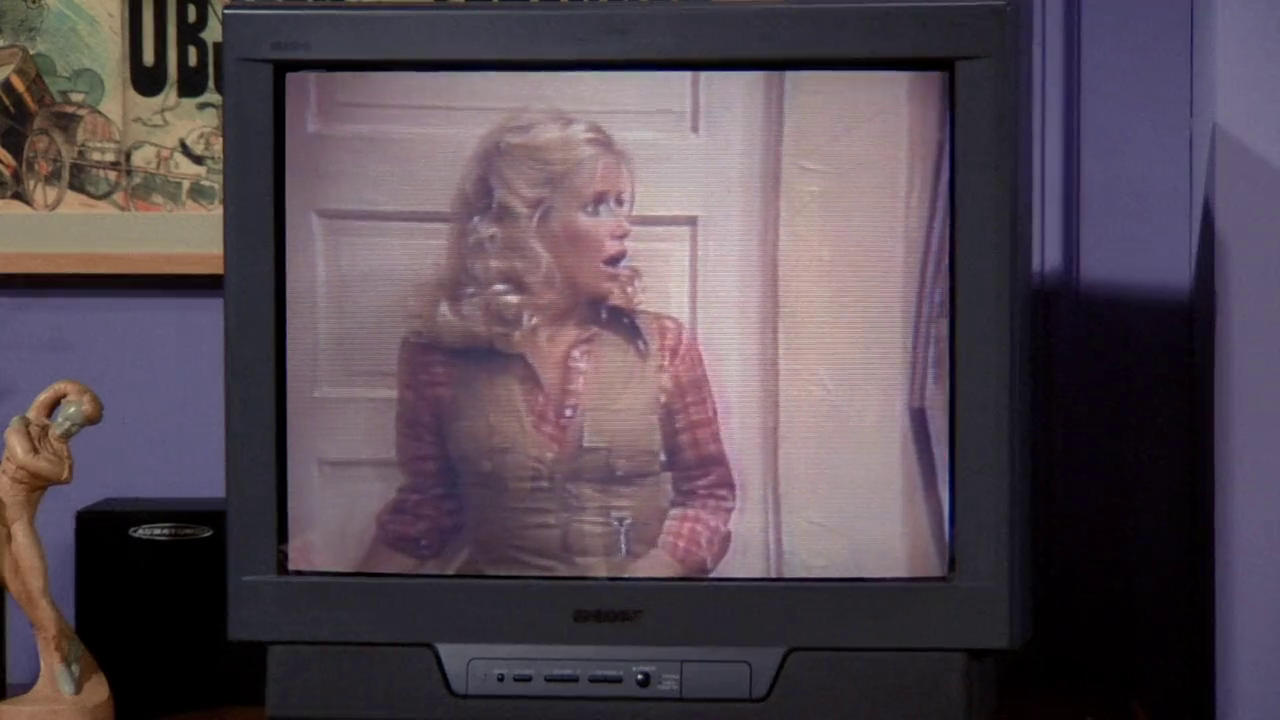
\includegraphics[trim={0 5cm 0 2cm,}, clip, width=\paperwidth]{./S01/img/2/threes-company.png}
    \caption{Three’s Company\label{fig:three-s-company}}
  \end{adjustwidth}
\end{figure}

\begin{tcolorbox}[enhanced,center upper,
    drop fuzzy shadow southeast, boxrule=0.3pt,
    lower separated=false,
    colframe=black!30!dialogoBorder,colback=white]
\begin{minipage}[c]{0.14\linewidth}
  \raisebox{\dimexpr-\height+\ht\strutbox\relax}{
    
\includegraphics[width=1.5cm]{./assets/img/chandler.png}
  }
   & \centering \scriptsize{Chandler}
\end{minipage}
\hspace{.1mm}
\begin{minipage}[c]{0.8\linewidth}
  \textbf{- I think this is the episode of Three's Company where's there's some kind of misunderstanding.}\\
  - Acho que este é o episódio de Three's Company onde há um mal-entendido.
\end{minipage}

\medskip
\begin{minipage}[c]{0.14\linewidth}
  \raisebox{\dimexpr-\height+\ht\strutbox\relax}{
    
\includegraphics[width=1.5cm]{./assets/img/phoebe.png}
  }
   & \centering \scriptsize{Phoebe}
\end{minipage}
\hspace{.1mm}
\begin{minipage}[c]{0.8\linewidth}
  \textbf{- Then I've already seen this one.}\\
  - Então, eu já vi.
\end{minipage}
\end{tcolorbox}

Chandler, Joey, Phoebe e Monica assistem a \emph{sitcom} \emph{Three's
Company} (1977-1984), conhecida no Brasil como \emph{Um é Pouco, Dois é
Bom e Três é Demais}. Conta a história de Janet e Chrissy que dividem um
apartamento em Santa Monica e conhecem um novo colega Jack. Ele estuda
gastronomia e, quando pedem para ele provar suas capacidades, finge ser
gay. Eles passam a morar juntos e passar por desentendimentos, aventuras
e brincadeiras. Daí a piada, o \emph{plot} da história quase sempre
envolve um desentendimento.

\begin{figure}
  \centering
  \begin{tikzpicture}
    \node [inner sep=0pt] at (0,0) {
      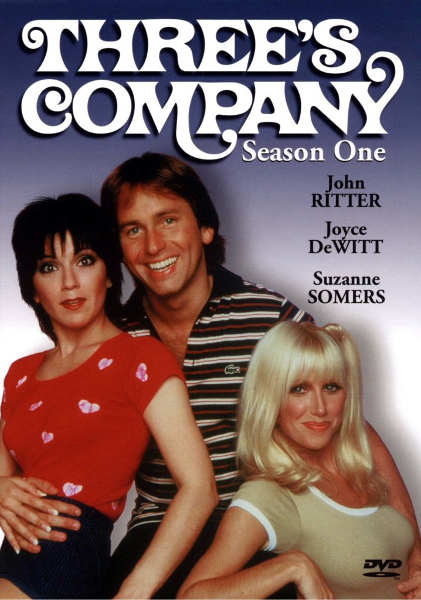
\includegraphics[width=0.4\textwidth,keepaspectratio]{./S01/img/2/threes-company-cover.jpg}
    };
    \draw [white, rounded corners=\ClipSep, line width=\ClipSep]
    (current bounding box.north west) --
    (current bounding box.north east) --
    (current bounding box.south east) --
    (current bounding box.south west) -- cycle
    ;
    \end{tikzpicture}
    \caption{Three’s Company - Cover\label{fig:three-s-company-cover}}
\end{figure}

\hypertarget{referuxeancias-1}{%
\subsection{Referências}\label{referuxeancias-1}}

\begin{itemize}
\tightlist
\item
  \sloppy Site oficial. \url{http://www.threescompany.com/}
\item
  \sloppy Fandom Wiki. \url{https://threescompany.fandom.com/wiki/Three%27s_Company}
\item
  \sloppy Página do Adoro Cinema. \url{http://www.adorocinema.com/series/serie-387/foto-detalhada/?cmediafile=21161912}
\end{itemize}

\hypertarget{thighmaster}{%
\section{Thighmaster}\label{thighmaster}}

\begin{figure}[!ht]
  \begin{adjustwidth}{-\oddsidemargin-1in}{-\rightmargin}
    \centering
    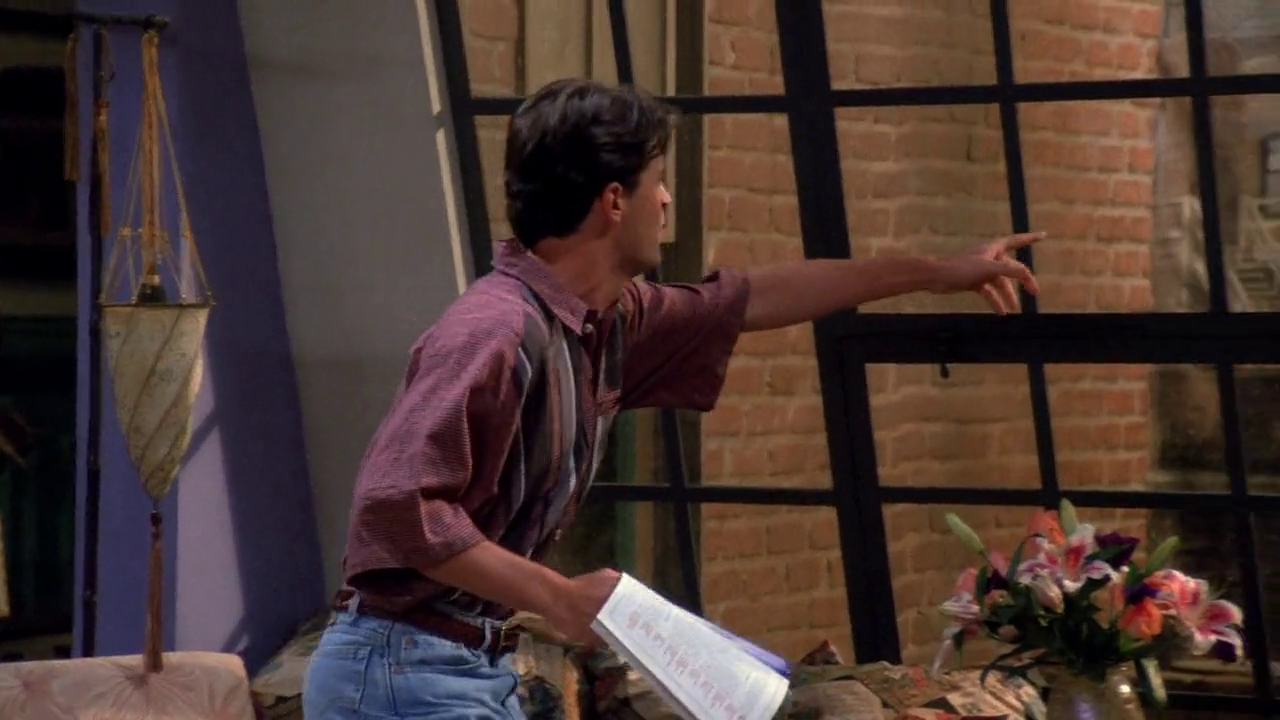
\includegraphics[trim={0 7cm 0 2cm,}, clip, width=\paperwidth]{./S01/img/2/thighmaster.png}
    \caption{Thighmaster\label{fig:thighmaster}}
  \end{adjustwidth}
\end{figure}

\begin{tcolorbox}[enhanced,center upper,
    drop fuzzy shadow southeast, boxrule=0.3pt,
    lower separated=false,
    colframe=black!30!dialogoBorder,colback=white]
\begin{minipage}[c]{0.14\linewidth}
  \raisebox{\dimexpr-\height+\ht\strutbox\relax}{
    
\includegraphics[width=1.5cm]{./assets/img/chandler.png}
  }
   & \centering \scriptsize{Chandler}
\end{minipage}
\hspace{.1mm}
\begin{minipage}[c]{0.8\linewidth}
  \textbf{- Ugly Naked Guy got a Thighmaster.}\\
  - Peladão feio fazendo exercício!
\end{minipage}
\end{tcolorbox}

Chandler menciona que o \emph{Ugly Naked Guy} está usando um
\emph{Thighmaster}, conhecido aparelho aeróbico usado para tonificar a
parte interna da coxa. O interessante aqui é que o \emph{Thighmaster}
está diretamente relacionado à seção \emph{Three's Company}, já que
Suzanne Somers - que faz o papel de Chrissy na série - é a porta voz
oficial do produto.

\begin{figure}
  \centering
  \begin{tikzpicture}
    \node [inner sep=0pt] at (0,0) {
      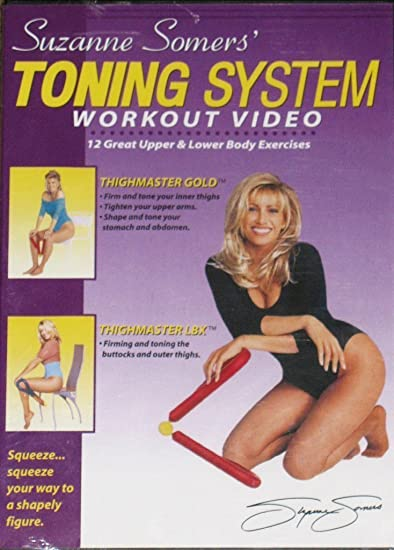
\includegraphics[width=0.3\textwidth,keepaspectratio]{./S01/img/2/suzanne-somers-thighmaster.jpg}
    };
    \draw [white, rounded corners=\ClipSep, line width=\ClipSep]
    (current bounding box.north west) --
    (current bounding box.north east) --
    (current bounding box.south east) --
    (current bounding box.south west) -- cycle
    ;
    \end{tikzpicture}
    \caption{Suzanne Somers - Thighmaster\label{fig:suzanne-somers-thighmaster}}
\end{figure}

\hypertarget{referuxeancias-2}{%
\subsection{Referências}\label{referuxeancias-2}}

\begin{itemize}
\tightlist
\item
  \sloppy Fandom Wiki - Thighmaster. \url{https://threescompany.fandom.com/wiki/Suzanne_Somers#Spokeswoman_for_Thighmaster}
\item
  \sloppy Trechos do comercial - YouTube. \url{https://www.youtube.com/watch?v=2yVeef8AnYI}
\end{itemize}

\hypertarget{in-the-kitchen-with-dinah}{%
\section{In the kitchen with\ldots{}
Dinah?}\label{in-the-kitchen-with-dinah}}

\begin{figure}[!ht]
  \begin{adjustwidth}{-\oddsidemargin-1in}{-\rightmargin}
    \centering
    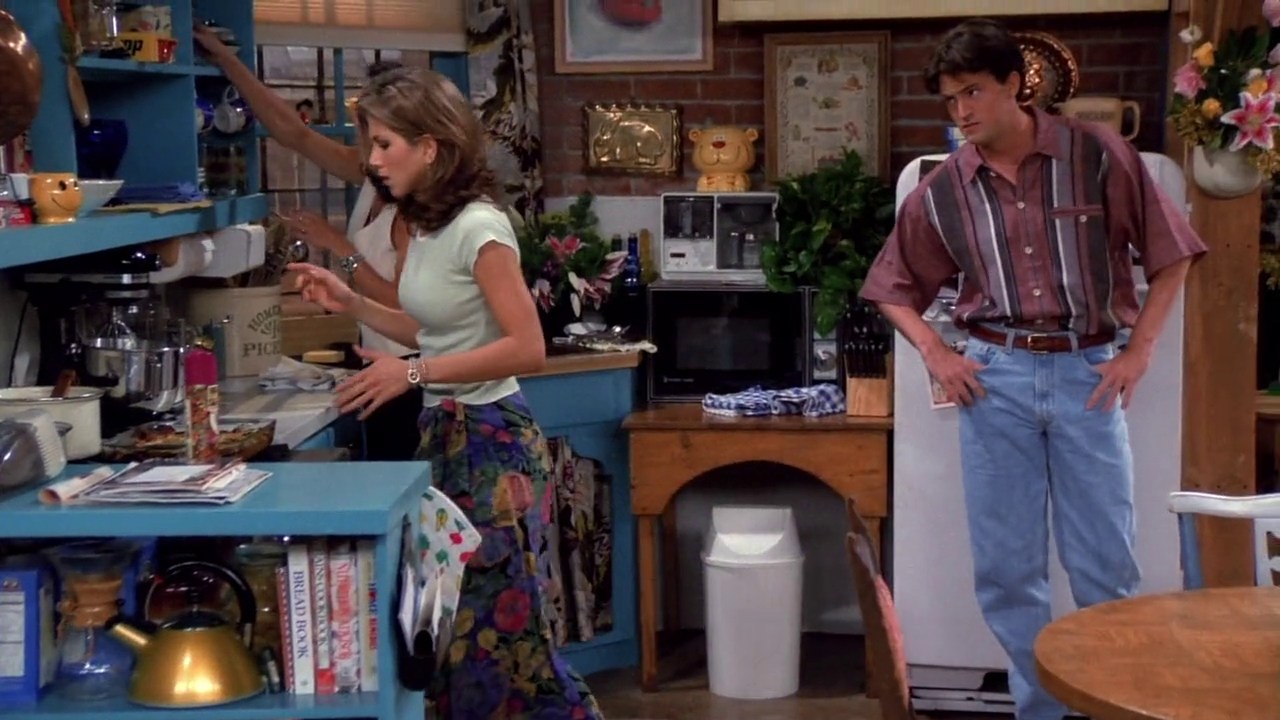
\includegraphics[trim={0 6cm 0 1cm,}, clip, width=\paperwidth]{./S01/img/2/kitchen-with-dinah.png}
    \caption{In the kitchen with… Dinah?\label{fig:in-the-kitchen-with-dinah}}
  \end{adjustwidth}
\end{figure}

\begin{tcolorbox}[enhanced,center upper,
    drop fuzzy shadow southeast, boxrule=0.3pt,
    lower separated=false,
    colframe=black!30!dialogoBorder,colback=white]
\begin{minipage}[c]{0.14\linewidth}
  \raisebox{\dimexpr-\height+\ht\strutbox\relax}{
    
\includegraphics[width=1.5cm]{./assets/img/rachel.png}
  }
   & \centering \scriptsize{Rachel}
\end{minipage}
\hspace{.1mm}
\begin{minipage}[c]{0.8\linewidth}
  \textbf{- I know I had it when I was in the kitchen with...}\\
  - Sei que estava com ela na cozinha com...
\end{minipage}

\medskip
\begin{minipage}[c]{0.14\linewidth}
  \raisebox{\dimexpr-\height+\ht\strutbox\relax}{
    
\includegraphics[width=1.5cm]{./assets/img/chandler.png}
  }
   & \centering \scriptsize{Chandler}
\end{minipage}
\hspace{.1mm}
\begin{minipage}[c]{0.8\linewidth}
  \textbf{- Dinah?}\\
  - Dinah?
\end{minipage}
\end{tcolorbox}

Enquanto procura sua aliança, Rachel menciona que estava na cozinha, e
Chandler pergunta se ela estava com Dinah. Isso é uma alusão a canção
folclórica \emph{I've Been Working on the Railroad} (C. 1894). Segue um
trecho da canção que é citado no diálogo:

\bigskip
\begin{tcolorbox}[enhanced,
    drop fuzzy shadow southeast, boxrule=0.3pt,
    lower separated=false, sidebyside, sidebyside align=top,
    halign=flush right, halign lower=left,
    colframe=black!30!dialogoBorder,colback=musicaBg]
\includegraphics[width=0.4cm]{./assets/img/icon-music.png}\\
Someone’s in the kitchen with Dinah\\Someone’s in the kitchen I know\\Someone’s in the kitchen with Dinah\\Strummin’ on the old banjo!\\
\tcblower
\includegraphics[width=0.4cm]{./assets/img/icon-language.png}\\
Alguém está na cozinha com Dinah\\Alguém está na cozinha eu sei\\Alguém está na cozinha com Dinah\\Dedilhando no velho banjo\\
\end{tcolorbox}

\hypertarget{referuxeancias-3}{%
\subsection{Referências}\label{referuxeancias-3}}

\begin{itemize}
\tightlist
\item
  \sloppy Live About - História da música (Inglês). \url{https://www.liveabout.com/ive-been-working-on-the-railroad-traditional-1322525}
\item
  \sloppy Versão por John Denver - YouTube. \url{https://www.youtube.com/watch?v=AAI6wjXEV6g}
\item
  \sloppy Every FRIENDS Joke - Blog. \url{https://every-friends-joke.blogspot.com/2017/06/when-i-was-in-kitchen-with-dinah.html}
\end{itemize}

\hypertarget{minnie-mouse}{%
\section{Minnie Mouse}\label{minnie-mouse}}

\begin{figure}[!ht]
  \begin{adjustwidth}{-\oddsidemargin-1in}{-\rightmargin}
    \centering
    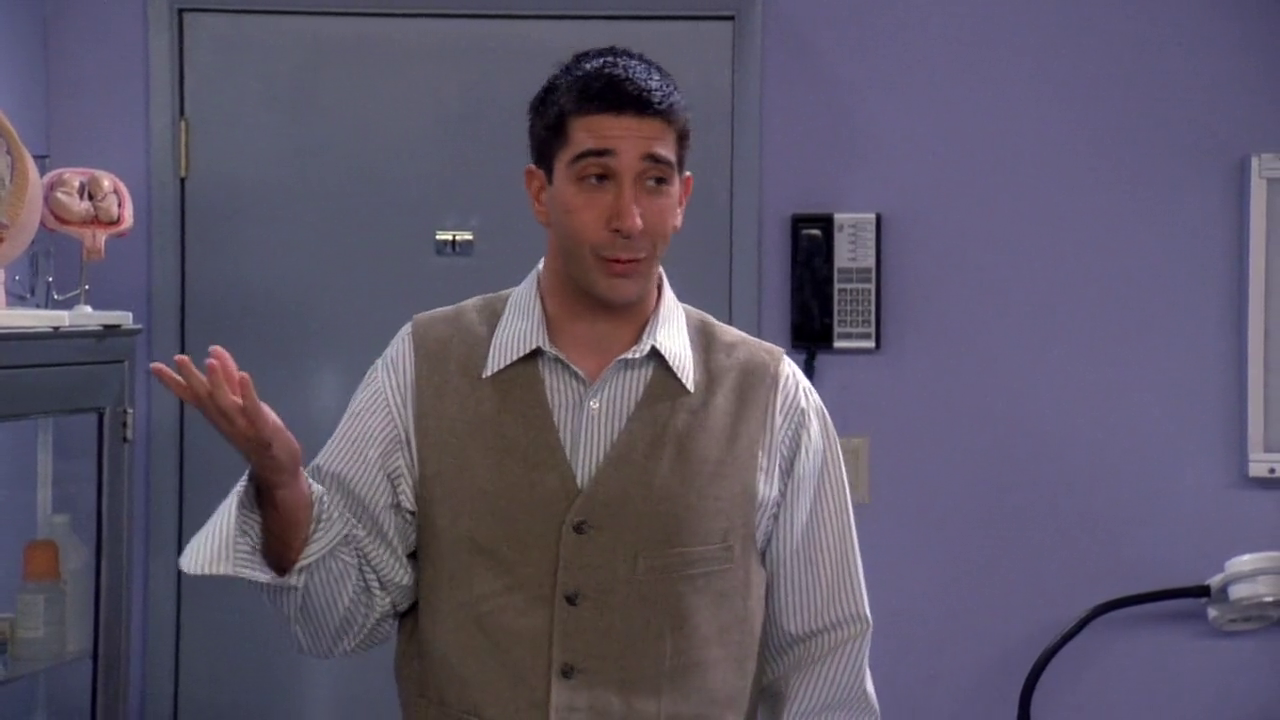
\includegraphics[trim={0 6cm 0 1cm,}, clip, width=\paperwidth]{./S01/img/2/minnie-mouse.png}
    \caption{Minnie Mouse\label{fig:minnie-mouse}}
  \end{adjustwidth}
\end{figure}

\begin{tcolorbox}[enhanced,center upper,
    drop fuzzy shadow southeast, boxrule=0.3pt,
    lower separated=false,
    colframe=black!30!dialogoBorder,colback=white]
\begin{minipage}[c]{0.14\linewidth}
  \raisebox{\dimexpr-\height+\ht\strutbox\relax}{
    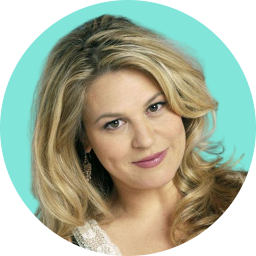
\includegraphics[width=1.5cm]{./assets/img/carol-1.png}
  }
   & \centering \scriptsize{Carol}
\end{minipage}
\hspace{.1mm}
\begin{minipage}[c]{0.8\linewidth}
  \textbf{- Minnie, if it's a girl.}\\
  - Minnie, se for menina.
\end{minipage}

\medskip
\begin{minipage}[c]{0.14\linewidth}
  \raisebox{\dimexpr-\height+\ht\strutbox\relax}{
    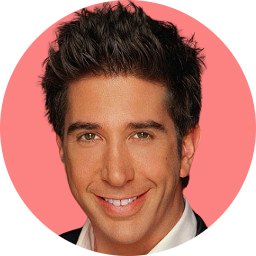
\includegraphics[width=1.5cm]{./assets/img/ross.png}
  }
   & \centering \scriptsize{Ross}
\end{minipage}
\hspace{.1mm}
\begin{minipage}[c]{0.8\linewidth}
  \textbf{- As in Mouse?}\\
  - Minnie Mouse?
\end{minipage}
\end{tcolorbox}

Ao discutir sobre o nome de seu filho com Carol e Susan, Ross menciona
\emph{Minnie Mouse,} famosa personagem de \emph{Walt Disney} criada em
1928. Aparece pela primeira vez no episódio \emph{Steamboat Willie}
(1928), já como a namorada de \emph{Mickey Mouse}.

\hypertarget{referuxeancias-4}{%
\subsection{Referências}\label{referuxeancias-4}}

\begin{itemize}
\tightlist
\item
  \sloppy Wikipédia. \url{https://pt.wikipedia.org/wiki/Minnie_Mouse}
\item
  \sloppy Steamboat Willie - YouTube. \url{https://www.youtube.com/watch?v=BBgghnQF6E4}
\end{itemize}

\hypertarget{enterprise}{%
\section{Enterprise}\label{enterprise}}

\begin{figure}[!ht]
  \begin{adjustwidth}{-\oddsidemargin-1in}{-\rightmargin}
    \centering
    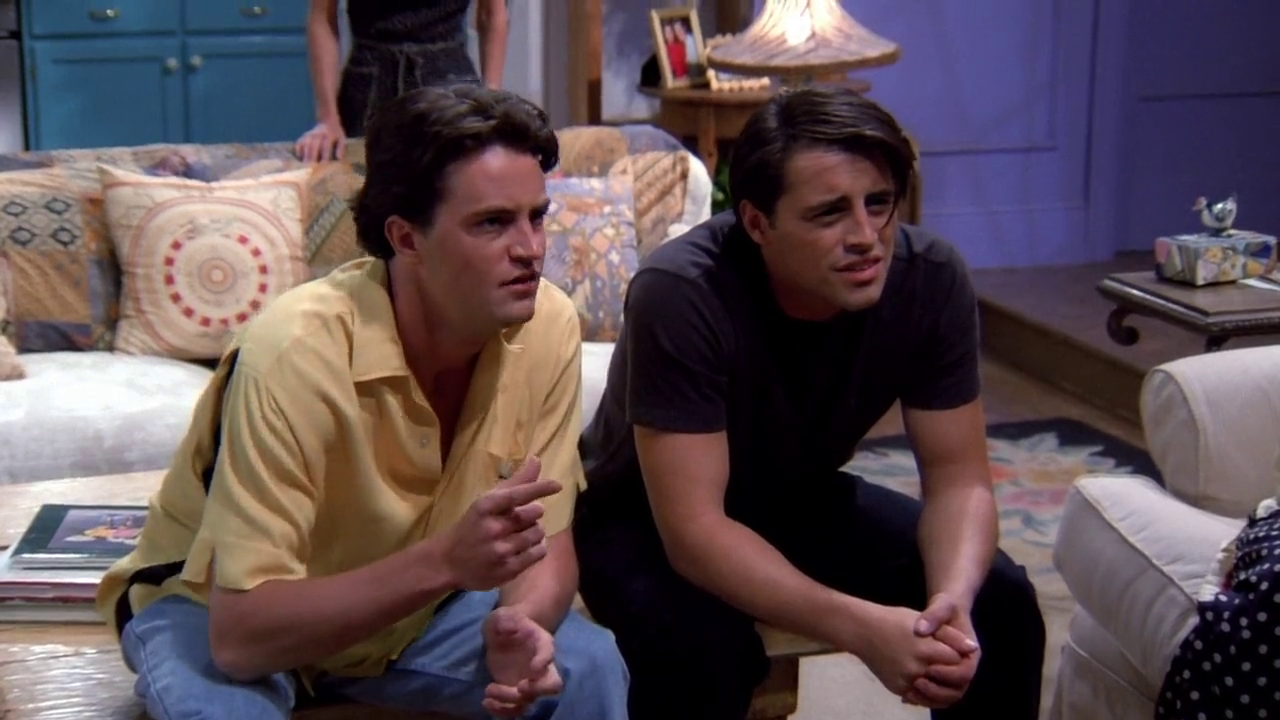
\includegraphics[trim={0 5cm 0 2cm,}, clip, width=\paperwidth]{./S01/img/2/enterprise.png}
    \caption{Enterprise\label{fig:enterprise}}
  \end{adjustwidth}
\end{figure}

\begin{tcolorbox}[enhanced,center upper,
    drop fuzzy shadow southeast, boxrule=0.3pt,
    lower separated=false,
    colframe=black!30!dialogoBorder,colback=white]
\begin{minipage}[c]{0.14\linewidth}
  \raisebox{\dimexpr-\height+\ht\strutbox\relax}{
    
\includegraphics[width=1.5cm]{./assets/img/joey.png}
  }
   & \centering \scriptsize{Joey}
\end{minipage}
\hspace{.1mm}
\begin{minipage}[c]{0.8\linewidth}
  \textbf{- What are we supposed to be seeing here?}\\
  - O que deveríamos ver?
\end{minipage}

\medskip
\begin{minipage}[c]{0.14\linewidth}
  \raisebox{\dimexpr-\height+\ht\strutbox\relax}{
    \includegraphics[width=1.5cm]{./assets/img/chandler.png}
  }
   & \centering \scriptsize{Chandler}
\end{minipage}
\hspace{.1mm}
\begin{minipage}[c]{0.8\linewidth}
  \textbf{- I don't know, but I think it's about to attack the Enterprise.}\\
  - Não sei, mas acho que vai atacar a Enterprise.
\end{minipage}
\end{tcolorbox}

Assistindo ao vídeo do ultrassom, Chandler faz uma piada comparando as
imagens a uma cena da séria \emph{Star Trek} (1966), e \emph{Enterprise}
é o nome da principal nave estelar. No Brasil a séria é conhecido como
\emph{Jornada nas Estrelas}.

\begin{figure}
  \centering
  \begin{tikzpicture}
    \node [inner sep=0pt] at (0,0) {
      \includegraphics[width=0.8\textwidth,keepaspectratio]{./S01/img/2/enterprise-ship.jpg}
    };
    \draw [white, rounded corners=\ClipSep, line width=\ClipSep]
    (current bounding box.north west) --
    (current bounding box.north east) --
    (current bounding box.south east) --
    (current bounding box.south west) -- cycle
    ;
    \end{tikzpicture}
    \caption{Enterprise\label{fig:enterprise}}
\end{figure}

\hypertarget{referuxeancias-5}{%
\subsection{Referências}\label{referuxeancias-5}}

\begin{itemize}
\tightlist
\item
  \sloppy Página oficial. \url{https://intl.startrek.com/database_article/enterprise-nx-01}
\item
  \sloppy Wikipédia. \url{https://pt.wikipedia.org/wiki/USS_Enterprise_(Star_Trek)}
\end{itemize}


\chapter{Aquele com o Dedão}

\textbf{RESUMO $\looparrowright$} Uma empresa de bebidas paga a Phoebe \$ 7.000 depois que ela encontra um dedo numa lata de refrigerante.

\begin{flushright}
\textcolor{gray600}{Exibido em Outubro, 05 1994}
\end{flushright}
\hypertarget{laurel-hardy}{%
\section{Laurel \& Hardy}\label{laurel-hardy}}

\begin{figure}[!ht]
  \begin{adjustwidth}{-\oddsidemargin-1in}{-\rightmargin}
    \centering
    \includegraphics[trim={0 7cm 0 2cm,}, clip, width=\paperwidth]{./S01/img/3/laurel-and-hardy.png}
    % \caption{Laurel & Hardy\label{fig:laurel-hardy}}
  \end{adjustwidth}
\end{figure}

No apartamento de Joey e Chandler, enquanto ensaiam para a audição, um
poster de \emph{Laurel \& Hardy} aparece na sala de estar. Esses
personagens são conhecidos no Brasil como \emph{O Gordo e o Magro} e
fizeram cerca de 106 filmes juntos, entre curtas-metragem sonoros e
mudos e filmes.

\hypertarget{referuxeancias}{%
\subsection{Referências}\label{referuxeancias}}

\begin{itemize}
\tightlist
\item
  \sloppy Site oficial. \url{http://www.laurel-and-hardy.com/}
\item
  \sloppy Wikipédia. \url{https://pt.wikipedia.org/wiki/Laurel_%26_Hardy}
\end{itemize}

\hypertarget{grand-jury-secrets}{%
\section{Grand Jury Secrets}\label{grand-jury-secrets}}

\begin{figure}[!ht]
  \begin{adjustwidth}{-\oddsidemargin-1in}{-\rightmargin}
    \centering
    \includegraphics[trim={0 6cm 0 3cm,}, clip, width=\paperwidth]{./S01/img/3/grand-jury-secrets.png}
    % \caption{Grand Jury Secrets\label{fig:grand-jury-secrets}}
  \end{adjustwidth}
\end{figure}

\emph{Grand Jury Secrets} (1939) é um filme de drama e mistério
americano. Conta a história de um repórter inescrupuloso que obtém
notícias através de um rádio escondido na sala de um júri, onde seu
irmão trabalha como advogado. O repórter é sequestrado e escapa devido
sua capacidade de transmitir sua situação.

\begin{figure}
  \centering
  \begin{tikzpicture}
    \node [inner sep=0pt] at (0,0) {
      \includegraphics[width=0.4\textwidth,keepaspectratio]{./S01/img/3/grand-jury-secrets-poster.jpg}
    };
    \draw [white, rounded corners=\ClipSep, line width=\ClipSep]
    (current bounding box.north west) --
    (current bounding box.north east) --
    (current bounding box.south east) --
    (current bounding box.south west) -- cycle
    ;
    \end{tikzpicture}
    \caption{Grand Jury Secrets poster\label{fig:grand-jury-secrets-poster}}
\end{figure}

\hypertarget{referuxeancias-1}{%
\subsection{Referências}\label{referuxeancias-1}}

\begin{itemize}
\tightlist
\item
  \sloppy BFI. \url{https://www.bfi.org.uk/films-tv-people/4ce2b6ab720c8}
\item
  \sloppy Loving The Classics. \url{https://www.lovingtheclassics.com/by-title/g/grand-jury-secrets-1939.html}
\item
  \sloppy IMDB. \url{https://www.imdb.com/title/tt0031390/}
\end{itemize}

\hypertarget{there-was-a-crooked-man}{%
\section{There was a crooked
man\ldots{}}\label{there-was-a-crooked-man}}

\begin{figure}[!ht]
  \begin{adjustwidth}{-\oddsidemargin-1in}{-\rightmargin}
    \centering
    \includegraphics[trim={0 7cm 0 2cm,}, clip, width=\paperwidth]{./S01/img/3/crooked-man.png}
    % \caption{There was a crooked man\label{fig:there-was-a-crooked-man}}
  \end{adjustwidth}
\end{figure}

\begin{tcolorbox}[enhanced,center upper,
    drop fuzzy shadow southeast, boxrule=0.3pt,
    lower separated=false,
    colframe=black!30!dialogoBorder,colback=white]
\begin{minipage}[c]{0.16\linewidth}
  \raisebox{\dimexpr-\height+\ht\strutbox\relax}{
    \centering \includegraphics[width=1.4cm]{./assets/img/phoebe.png}
  }
   & \centering \scriptsize{Phoebe}
\end{minipage}
\hfill
\begin{minipage}[c]{0.8\linewidth}
  \textbf{- From the nursery rhyme. 'There was a crooked man, Who had a crooked smile, Who lived in a shoe, For a... while...'}\\
  - Da musiquinha. 'Havia um cara de sorriso torto. E morava no sapato, por um... tempo...
\end{minipage}
\end{tcolorbox}

Enquanto os amigos discutem o quanto Alan é legal, Phoebe o compara com
o homem no sapato, que, como Joey notou, tem um sorisso torto. A
``musiquinha'' ou canção de ninar é \emph{There Was a Crooked Man} (C.
1840) de origem desconhecida.

Letra original e tradução da canção:

\bigskip
\begin{tcolorbox}[enhanced,
    drop fuzzy shadow southeast, boxrule=0.3pt,
    lower separated=false, sidebyside, sidebyside align=top,
    halign=flush right, halign lower=left,
    colframe=black!30!dialogoBorder,colback=musicaBg]
\includegraphics[width=0.4cm]{./assets/img/icon-music.png}\\
There was a crooked man, and he walked a crooked mile.\\He found a crooked sixpence upon a crooked stile.\\He bought a crooked cat, which caught a crooked mouse,\\And they all lived together in a little crooked house.\\
\tcblower
\includegraphics[width=0.4cm]{./assets/img/icon-language.png}\\
Havia um homem torto, e ele andou em uma estrada torta\\Ele encontrou uma moeda torta sobre um rebordo torto\\Ele comprou um gato torto, que pegou um rato torto\\E eles todos viveram juntos em uma pequena casa torta\\
\end{tcolorbox}

\hypertarget{referuxeancias-2}{%
\subsection{Referências}\label{referuxeancias-2}}

\begin{itemize}
\tightlist
\item
  \sloppy Wikipédia. \url{https://en.wikipedia.org/wiki/There_Was_a_Crooked_Man}
\item
  \sloppy There Was A Crooked Man Nursery Rhyme - YouTube. \url{https://www.youtube.com/watch?v=WqyUOlz_6i4}
\item
  Alchin, Linda Kathryn. \emph{Secret History of Nursery Rhymes.} Linda
  Alchin, 2010.
\end{itemize}

\hypertarget{david-hasselhoff}{%
\section{David Hasselhoff}\label{david-hasselhoff}}

\begin{figure}[!ht]
  \begin{adjustwidth}{-\oddsidemargin-1in}{-\rightmargin}
    \centering
    \includegraphics[trim={0 6cm 0 2cm,}, clip, width=\paperwidth]{./S01/img/3/david-hasselhoff.png}
    % \caption{David Hasselhoff\label{fig:david-hasselhoff}}
  \end{adjustwidth}
\end{figure}

\begin{tcolorbox}[enhanced,center upper,
    drop fuzzy shadow southeast, boxrule=0.3pt,
    lower separated=false,
    colframe=black!30!dialogoBorder,colback=white]
\begin{minipage}[c]{0.16\linewidth}
  \raisebox{\dimexpr-\height+\ht\strutbox\relax}{
    \centering \includegraphics[width=1.4cm]{./assets/img/chandler.png}
  }
   & \centering \scriptsize{Chandler}
\end{minipage}
\hfill
\begin{minipage}[c]{0.8\linewidth}
  \textbf{- I'd marry him just for his David Hasselhoff impression alone.}\\
  - Eu casaria por causa da imitação de David Hasselholff.
\end{minipage}
\end{tcolorbox}

\emph{David Hasselhoff} é ator, cantor, produtor e empresário
norte-americano. Um de seus grandes papeis de sucesso foi o salva-vidas
\emph{Mitch Buchannon} em \emph{Baywatch} (1989 - 2001), conhecida no
Brasil como \emph{S.O.S. Malibu}, série que acaba sendo conhecida como a
preferida de Joey no episódio
\textbf{\textcolor{primarycolor}{S03E06 - Aquele do flashback}}, em que
ele apresenta a série a Chandler.

\begin{figure}
  \centering
  \begin{tikzpicture}
    \node [inner sep=0pt] at (0,0) {
      \includegraphics[width=0.8\textwidth,keepaspectratio]{./S01/img/3/david-hasselhoff-baywatch.jpg}
    };
    \draw [white, rounded corners=\ClipSep, line width=\ClipSep]
    (current bounding box.north west) --
    (current bounding box.north east) --
    (current bounding box.south east) --
    (current bounding box.south west) -- cycle
    ;
    \end{tikzpicture}
    \caption{David Hasselhoff em Baywatch\label{fig:david-hasselhoff-em-baywatch}}
\end{figure}

\hypertarget{referuxeancias-3}{%
\subsection{Referências}\label{referuxeancias-3}}

\begin{itemize}
\tightlist
\item
  \sloppy IMDB. \url{https://www.imdb.com/name/nm0001327/}
\item
  \sloppy Site oficial Baywatch. \url{https://www.baywatch.com/}
\end{itemize}

\hypertarget{bugs-bunny}{%
\section{Bugs Bunny}\label{bugs-bunny}}

\begin{figure}[!ht]
  \begin{adjustwidth}{-\oddsidemargin-1in}{-\rightmargin}
    \centering
    \includegraphics[trim={0 7cm 0 2cm,}, clip, width=\paperwidth]{./S01/img/3/bugs-bunny.png}
    % \caption{Bugs Bunny\label{fig:bugs-bunny}}
  \end{adjustwidth}
\end{figure}

\begin{tcolorbox}[enhanced,center upper,
    drop fuzzy shadow southeast, boxrule=0.3pt,
    lower separated=false,
    colframe=black!30!dialogoBorder,colback=white]
\begin{minipage}[c]{0.16\linewidth}
  \raisebox{\dimexpr-\height+\ht\strutbox\relax}{
    \centering \includegraphics[width=1.4cm]{./assets/img/ross.png}
  }
   & \centering \scriptsize{Ross}
\end{minipage}
\hfill
\begin{minipage}[c]{0.8\linewidth}
  \textbf{- He was like that Bugs Bunny cartoon where Bugs is playing all the positions.}\\
  - Ele parecia o Pernalonga no desenho em que jogava em todas as posições.
\end{minipage}
\end{tcolorbox}

Enquanto explica como Alan joga bem \emph{softball}, Ross menciona
\emph{Bugs Bunny}, conhecido no Brasil como \emph{Pernalonga},
personagem da \emph{Looney Tunes}. O episódio citado por Ross é o
\emph{Baseball Bugs} (1946).

\begin{figure}
  \centering
  \begin{tikzpicture}
    \node [inner sep=0pt] at (0,0) {
      \includegraphics[width=0.4\textwidth,keepaspectratio]{./S01/img/3/baseball-bugs.jpg}
    };
    \draw [white, rounded corners=\ClipSep, line width=\ClipSep]
    (current bounding box.north west) --
    (current bounding box.north east) --
    (current bounding box.south east) --
    (current bounding box.south west) -- cycle
    ;
    \end{tikzpicture}
    \caption{Baseball Bugs\label{fig:baseball-bugs}}
\end{figure}

\hypertarget{referuxeancias-4}{%
\subsection{Referências}\label{referuxeancias-4}}

\begin{itemize}
\tightlist
\item
  \sloppy Fandom Wiki - Looney Tunes. \url{https://looneytunes.fandom.com/wiki/Baseball_Bugs}
\item
  \sloppy IMDB. \url{https://www.imdb.com/title/tt0038333/}
\item
  \sloppy Episódio na SuperCartoons (Inglês). \url{https://www.supercartoons.net/cartoon/629/bugs-bunny-baseball-bugs.html}
\item
  \sloppy Diferenças entre softball e baseball (Inglês). \url{https://www.dummies.com/sports/fantasy-sports/fantasy-baseball/the-differences-between-softball-and-baseball/}
\end{itemize}

\hypertarget{lamb-chop}{%
\section{Lamb Chop}\label{lamb-chop}}

\begin{figure}[!ht]
  \begin{adjustwidth}{-\oddsidemargin-1in}{-\rightmargin}
    \centering
    \includegraphics[trim={0 6cm 0 3cm,}, clip, width=\paperwidth]{./S01/img/3/lamb-chop.png}
    % \caption{Lamb Chop\label{fig:lamb-chop}}
  \end{adjustwidth}
\end{figure}

\begin{tcolorbox}[enhanced,center upper,
    drop fuzzy shadow southeast, boxrule=0.3pt,
    lower separated=false,
    colframe=black!30!dialogoBorder,colback=white]
\begin{minipage}[c]{0.16\linewidth}
  \raisebox{\dimexpr-\height+\ht\strutbox\relax}{
    \centering \includegraphics[width=1.4cm]{./assets/img/chandler.png}
  }
   & \centering \scriptsize{Chandler}
\end{minipage}
\hfill
\begin{minipage}[c]{0.8\linewidth}
  \textbf{- If I had a sock on my hand for 30 years, it'd be talking too.}\\
  - Se eu usasse uma meia na mão por 30 anos, ela também ia falar.
\end{minipage}
\end{tcolorbox}

No apartamento de Monica os amigos assistem a \emph{Lamb Chop}, fantoche
criado por \emph{Shari Lewis} (1934-1998). Sua filha, \emph{Mallory
Lewis}, continuou seu legado e faz performances de \emph{Lamb Chop} até
hoje.

\begin{figure}
  \centering
  \begin{tikzpicture}
    \node [inner sep=0pt] at (0,0) {
      \includegraphics[width=0.7\textwidth,keepaspectratio]{./S01/img/3/shari-lewis.jpg}
    };
    \draw [white, rounded corners=\ClipSep, line width=\ClipSep]
    (current bounding box.north west) --
    (current bounding box.north east) --
    (current bounding box.south east) --
    (current bounding box.south west) -- cycle
    ;
    \end{tikzpicture}
    \caption{Shari Lewis\label{fig:shari-lewis}}
\end{figure}

\hypertarget{referuxeancias-5}{%
\subsection{Referências}\label{referuxeancias-5}}

\begin{itemize}
\tightlist
\item
  \sloppy Site oficial. \url{https://mallorylewisandlambchop.com/faqs/}
\end{itemize}


\chapter{Aquele com George Stephanopoulus}

\textbf{RESUMO $\looparrowright$} Um entregador acidentalmente leva uma pizza que deveria ser entregue a George Stephanopoulos, que mora em frente às meninas.

\begin{flushright}
\textcolor{gray600}{Exibido em Outubro, 12 1994}
\end{flushright}
\hypertarget{dairy-queen}{%
\section{Dairy Queen}\label{dairy-queen}}

\begin{figure}[!ht]
  \begin{adjustwidth}{-\oddsidemargin-1in}{-\rightmargin}
    \centering
    \includegraphics[trim={0 7cm 0 2cm,}, clip, width=\paperwidth]{./S01/img/4/dairy-queen.png}
    % \caption{Dairy Queen\label{fig:dairy-queen}}
  \end{adjustwidth}
\end{figure}

\begin{tcolorbox}[enhanced,center upper,
    drop fuzzy shadow southeast, boxrule=0.3pt,
    lower separated=false, breakable,
    colframe=black!30!dialogoBorder,colback=white]
\begin{minipage}[c]{0.16\linewidth}
  \raisebox{\dimexpr-\height+\ht\strutbox\relax}{
    \centering \includegraphics[width=1.4cm]{./assets/img/phoebe.png}
  }
   & \centering \scriptsize{Phoebe}
\end{minipage}
\hfill
\begin{minipage}[c]{0.8\linewidth}
  \textbf{- There was a cave-in in one of the mines, and eight people were killed.}\\
  - Uma mina desabou e oito pessoas morreram.
\end{minipage}

\medskip
\begin{minipage}[c]{0.16\linewidth}
  \raisebox{\dimexpr-\height+\ht\strutbox\relax}{
    \centering \includegraphics[width=1.4cm]{./assets/img/monica.png}
  }
   & \centering \scriptsize{Monica}
\end{minipage}
\hfill
\begin{minipage}[c]{0.8\linewidth}
  \textbf{- Wow, you worked in a mine?}\\
  - Trabalhou em uma mina?
\end{minipage}

\medskip
\begin{minipage}[c]{0.16\linewidth}
  \raisebox{\dimexpr-\height+\ht\strutbox\relax}{
    \centering \includegraphics[width=1.4cm]{./assets/img/phoebe.png}
  }
   & \centering \scriptsize{Phoebe}
\end{minipage}
\hfill
\begin{minipage}[c]{0.8\linewidth}
  \textbf{- No, I worked at a Dairy Queen. Why?}\\
  - Não, em um Dairy Queen. Por quê?
\end{minipage}
\end{tcolorbox}

Enquanto discutem sobre empregos e salários, Phoebe menciona um de seus
empregos em uma mina. Monica fica abismada com o fato e quer saber se
aquilo era verdade. Phoebe, sarcasticamente, responde que não, na
verdade era um \emph{Dairy Queen}. \footnote{\sloppy Site oficial. \url{https://dairyqueen.com/}}

\emph{Dairy Queen} (1940) é uma famosa rede de sorveterias e
restaurantes de \emph{fast-food}.

\hypertarget{rachel-has-left-the-building}{%
\section{Rachel has left the
building}\label{rachel-has-left-the-building}}

\begin{figure}[!ht]
  \begin{adjustwidth}{-\oddsidemargin-1in}{-\rightmargin}
    \centering
    \includegraphics[trim={0 6cm 0 2cm,}, clip, width=\paperwidth]{./S01/img/4/rachel-has-left-the-building.png}
    % \caption{Rachel has left the building\label{fig:rachel-has-left-the-building}}
  \end{adjustwidth}
\end{figure}

\begin{tcolorbox}[enhanced,center upper,
    drop fuzzy shadow southeast, boxrule=0.3pt,
    lower separated=false, breakable,
    colframe=black!30!dialogoBorder,colback=white]
\begin{minipage}[c]{0.16\linewidth}
  \raisebox{\dimexpr-\height+\ht\strutbox\relax}{
    \centering \includegraphics[width=1.4cm]{./assets/img/monica.png}
  }
   & \centering \scriptsize{Monica}
\end{minipage}
\hfill
\begin{minipage}[c]{0.8\linewidth}
  \textbf{- Rachel has left the building.}\\
  - Rachel deixou o edifício.
\end{minipage}
\end{tcolorbox}

Após atender a um telefonema da operadora de cartão perguntando sobre a
Rachel, Monica diz a frase \emph{Rachel has left the building}. Isto é
uma paráfrase de \emph{Elvis has left the building}. Era uma frase usada
para dispersar o público que ficava a espera do bis ao final do show do
Rei do \emph{Rock and Roll Elvis Presley}. \footnote{\sloppy Fandom Wiki. \url{https://friends.fandom.com/wiki/The_One_With_George_Stephanopoulos}}
\footnote{\sloppy Wikipédia. \url{https://en.wikipedia.org/wiki/Elvis_has_left_the_building}}

\hypertarget{jack-and-the-beanstalk}{%
\section{Jack and the Beanstalk}\label{jack-and-the-beanstalk}}

\begin{figure}[!ht]
  \begin{adjustwidth}{-\oddsidemargin-1in}{-\rightmargin}
    \centering
    \includegraphics[trim={0 6cm 0 2cm,}, clip, width=\paperwidth]{./S01/img/4/jack-and-the-beanstalk.png}
    % \caption{Jack and the Beanstalk\label{fig:jack-and-the-beanstalk}}
  \end{adjustwidth}
\end{figure}

\begin{tcolorbox}[enhanced,center upper,
    drop fuzzy shadow southeast, boxrule=0.3pt,
    lower separated=false, breakable,
    colframe=black!30!dialogoBorder,colback=white]
\begin{minipage}[c]{0.16\linewidth}
  \raisebox{\dimexpr-\height+\ht\strutbox\relax}{
    \centering \includegraphics[width=1.4cm]{./assets/img/phoebe.png}
  }
   & \centering \scriptsize{Phoebe}
\end{minipage}
\hfill
\begin{minipage}[c]{0.8\linewidth}
  \textbf{- You are just like Jack.}\\
  - Você é igual ao João.
\end{minipage}

\medskip
\begin{minipage}[c]{0.16\linewidth}
  \raisebox{\dimexpr-\height+\ht\strutbox\relax}{
    \centering \includegraphics[width=1.4cm]{./assets/img/rachel.png}
  }
   & \centering \scriptsize{Rachel}
\end{minipage}
\hfill
\begin{minipage}[c]{0.8\linewidth}
  \textbf{- Jack from downstairs?}\\
  - João, do andar de baixo?
\end{minipage}

\medskip
\begin{minipage}[c]{0.16\linewidth}
  \raisebox{\dimexpr-\height+\ht\strutbox\relax}{
    \centering \includegraphics[width=1.4cm]{./assets/img/phoebe.png}
  }
   & \centering \scriptsize{Phoebe}
\end{minipage}
\hfill
\begin{minipage}[c]{0.8\linewidth}
  \textbf{- No, Jack and the Beanstalk.}\\
  - Não, João e o Pé de Feijão.
\end{minipage}
\end{tcolorbox}

\emph{Jack and the Beanstalk} (1807), conhecido no Brasil como
\emph{João e o Pé de Feijão}, é um conto de fadas de origem inglesa. A
Phoebe conta bem o enredo da história na cena. É uma história bastante
conhecida e referenciada diversas vezes, como em \emph{O Pica-pau},
\emph{Mickey Mouse}, entre outros.\footnote{\sloppy Página da Universidade de Pittsburgh (Inglês). \url{https://www.pitt.edu/~dash/type0328jack.html}}

\hypertarget{george-stephanopoulos}{%
\section{George Stephanopoulos}\label{george-stephanopoulos}}

\begin{figure}[!ht]
  \begin{adjustwidth}{-\oddsidemargin-1in}{-\rightmargin}
    \centering
    \includegraphics[trim={0 10cm 0 3cm,}, clip, width=\paperwidth]{./S01/img/4/george-stephanopoulos.png}
    % \caption{George Stephanopoulos\label{fig:george-stephanopoulos}}
  \end{adjustwidth}
\end{figure}

\begin{tcolorbox}[enhanced,center upper,
    drop fuzzy shadow southeast, boxrule=0.3pt,
    lower separated=false, breakable,
    colframe=black!30!dialogoBorder,colback=white]
\begin{minipage}[c]{0.16\linewidth}
  \raisebox{\dimexpr-\height+\ht\strutbox\relax}{
    \centering \includegraphics[width=1.4cm]{./assets/img/monica.png}
  }
   & \centering \scriptsize{Monica}
\end{minipage}
\hfill
\begin{minipage}[c]{0.8\linewidth}
  \textbf{- Did you say G. Stephanopoulos?}\\
  - Calma, você falou G. Stephanopoulos?
\end{minipage}
\end{tcolorbox}

\emph{George Stephanopoulos} (1961-) \footnote{\sloppy Twitter. \url{https://twitter.com/gstephanopoulos}}
realmente existe e na época dessa temporada era diretor de comunicações
da campanha presidencial de Bill Clinton. Atualmente é, entre outras
coisas, âncora do telejornal \emph{Good Morning America}.\footnote{\sloppy IMDB. \url{https://www.imdb.com/name/nm0826888/?ref_=tt_ov_st_sm}}

Essa passagem de sua vida virou o documentário \emph{The War Room}
(1993).\footnote{\sloppy IMDB Documentário. \url{https://www.imdb.com/title/tt0108515/}}

\begin{figure}
  \centering
  \begin{tikzpicture}
    \node [inner sep=0pt] at (0,0) {
      \includegraphics[width=0.6\textwidth,keepaspectratio]{./S01/img/4/george-stephanopoulos-war-room.jpg}
    };
    \draw [white, rounded corners=\ClipSep, line width=\ClipSep]
    (current bounding box.north west) --
    (current bounding box.north east) --
    (current bounding box.south east) --
    (current bounding box.south west) -- cycle
    ;
    \end{tikzpicture}
    \caption{George Stephanopoulos - The War Room\label{fig:george-stephanopoulos-the-war-room}}
\end{figure}

\hypertarget{george-snuffleupagus}{%
\section{George ``Snuffleupagus''}\label{george-snuffleupagus}}

\begin{figure}[!ht]
  \begin{adjustwidth}{-\oddsidemargin-1in}{-\rightmargin}
    \centering
    \includegraphics[trim={0 8cm 0 1cm,}, clip, width=\paperwidth]{./S01/img/4/george-snuffleupagus.png}
    % \caption{George ``Snuffleupagus''\label{fig:george-snuffleupagus}}
  \end{adjustwidth}
\end{figure}

\begin{tcolorbox}[enhanced,center upper,
    drop fuzzy shadow southeast, boxrule=0.3pt,
    lower separated=false, breakable,
    colframe=black!30!dialogoBorder,colback=white]
\begin{minipage}[c]{0.16\linewidth}
  \raisebox{\dimexpr-\height+\ht\strutbox\relax}{
    \centering \includegraphics[width=1.4cm]{./assets/img/rachel.png}
  }
   & \centering \scriptsize{Rachel}
\end{minipage}
\hfill
\begin{minipage}[c]{0.8\linewidth}
  \textbf{- Who's George Snuffleupagus?}\\
  - Quem é George Snuffleupagus?
\end{minipage}

\medskip
\begin{minipage}[c]{0.16\linewidth}
  \raisebox{\dimexpr-\height+\ht\strutbox\relax}{
    \centering \includegraphics[width=1.4cm]{./assets/img/phoebe.png}
  }
   & \centering \scriptsize{Phoebe}
\end{minipage}
\hfill
\begin{minipage}[c]{0.8\linewidth}
  \textbf{- That's Big Bird's friend.}\\
  - Amigo do Garibaldo.
\end{minipage}
\end{tcolorbox}

Rachel confunde o sobrenome de George e o chama de \emph{Snuffleupagus}
\footnote{\sloppy Fandom Wiki - Mr. Snuffleupagus. \url{https://muppet.fandom.com/wiki/Mr._Snuffleupagus}}.
Ele é realmente amigo de \emph{Big Bird} \footnote{\sloppy Fandom Wiki - Big Bird. \url{https://muppet.fandom.com/wiki/Big_Bird}}
e, ambos, fazem parte do programa de televisão educacional \emph{Sesame
Street} (1969), conhecido no Brasil como \emph{Vila Sésamo} \footnote{\sloppy Sesame Street - Site oficial. \url{https://www.sesamestreet.org/}}.
Em nossa versão, \emph{Snuffleupagus} era \emph{Funga-Funga} (à direita)
e \emph{Big Bird} era \emph{Garibaldo} (à esquerda).

\begin{figure}
  \centering
  \begin{tikzpicture}
    \node [inner sep=0pt] at (0,0) {
      \includegraphics[width=0.5\textwidth,keepaspectratio]{./S01/img/4/snuffleupagus-big-bird.jpg}
    };
    \draw [white, rounded corners=\ClipSep, line width=\ClipSep]
    (current bounding box.north west) --
    (current bounding box.north east) --
    (current bounding box.south east) --
    (current bounding box.south west) -- cycle
    ;
    \end{tikzpicture}
    \caption{Snuffleupagus e Big Bird\label{fig:snuffleupagus-e-big-bird}}
\end{figure}

\hypertarget{silence-of-the-lambs}{%
\section{Silence of the Lambs}\label{silence-of-the-lambs}}

\begin{figure}[!ht]
  \begin{adjustwidth}{-\oddsidemargin-1in}{-\rightmargin}
    \centering
    \includegraphics[trim={0 8cm 0 3cm,}, clip, width=\paperwidth]{./S01/img/4/silence-of-the-lambs.png}
    % \caption{Silence of the Lambs\label{fig:silence-of-the-lambs}}
  \end{adjustwidth}
\end{figure}

\begin{tcolorbox}[enhanced,center upper,
    drop fuzzy shadow southeast, boxrule=0.3pt,
    lower separated=false, breakable,
    colframe=black!30!dialogoBorder,colback=white]
\begin{minipage}[c]{0.16\linewidth}
  \raisebox{\dimexpr-\height+\ht\strutbox\relax}{
    \centering \includegraphics[width=1.4cm]{./assets/img/chandler.png}
  }
   & \centering \scriptsize{Chandler}
\end{minipage}
\hfill
\begin{minipage}[c]{0.8\linewidth}
  \textbf{- Oh, I thought you were great in Silence of the Lambs.}\\
  - Você estava ótimo em Silêncio dos Inocentes.
\end{minipage}
\end{tcolorbox}

\emph{Silence of the Lambs} (1991) é um filme norte-americano de
suspense, drama e terror, estrelado por \emph{Jodie Foster} e
\emph{Anthony Hopkins}. A comparação feita por Chandler se refere ao
modo como o \emph{Dr.~Hannibal Lecter}, interpretado por \emph{Hopkins},
era transportado quando precisava sair da cadeia. No Brasil o filme
ficou conhecido como \emph{Silêncio dos Inocentes}.\footnote{\sloppy The Silence of the Lambs - IMDB. \url{https://www.imdb.com/title/tt0102926/}}

\begin{figure}
  \centering
  \begin{tikzpicture}
    \node [inner sep=0pt] at (0,0) {
      \includegraphics[width=0.5\textwidth,keepaspectratio]{./S01/img/4/hannibal-lecter.jpg}
    };
    \draw [white, rounded corners=\ClipSep, line width=\ClipSep]
    (current bounding box.north west) --
    (current bounding box.north east) --
    (current bounding box.south east) --
    (current bounding box.south west) -- cycle
    ;
    \end{tikzpicture}
    \caption{Hannibal Lecter\label{fig:hannibal-lecter}}
\end{figure}


\chapter{Aquele com o Sabão em Pó da Alemanha Oriental}

\textbf{RESUMO $\looparrowright$} Ross ajuda Rachel a lavar a roupa e considera o evento um primeiro encontro. Joey faz com que Monica se passe como sua nova namorada.

\begin{flushright}
\textcolor{gray600}{Exibido em Outubro, 19 1994}
\end{flushright}
\hypertarget{bullwinkle-socks}{%
\section{Bullwinkle socks}\label{bullwinkle-socks}}

\begin{figure}[!ht]
  \begin{adjustwidth}{-\oddsidemargin-1in}{-\rightmargin}
    \centering
    \includegraphics[trim={0 4cm 0 3cm,}, clip, width=\paperwidth]{./S01/img/5/bullwinkle-socks.png}
    % \caption{Bullwinkle socks\label{fig:bullwinkle-socks}}
  \end{adjustwidth}
\end{figure}

\begin{tcolorbox}[enhanced,center upper,
    drop fuzzy shadow southeast, boxrule=0.3pt,
    lower separated=false, breakable,
    colframe=black!30!dialogoBorder,colback=white]
\begin{minipage}[c]{0.16\linewidth}
  \raisebox{\dimexpr-\height+\ht\strutbox\relax}{
    \centering \includegraphics[width=1.4cm]{./assets/img/janice.png}
  }
   & \centering \scriptsize{Janice}
\end{minipage}
\hfill
\begin{minipage}[c]{0.8\linewidth}
  \textbf{- I got you... these.}\\
  - Comprei... isto.
\end{minipage}

\medskip
\begin{minipage}[c]{0.16\linewidth}
  \raisebox{\dimexpr-\height+\ht\strutbox\relax}{
    \centering \includegraphics[width=1.4cm]{./assets/img/chandler.png}
  }
   & \centering \scriptsize{Chandler}
\end{minipage}
\hfill
\begin{minipage}[c]{0.8\linewidth}
  \textbf{- Bullwinkle socks.}\\
  - Uma meia do Alceu.
\end{minipage}
\end{tcolorbox}

\saveparinfos
\noindent
\begin{minipage}[c]{0.5\textwidth}\useparinfo

Para o dia dos namorados, Janice compra para Chandler meias do
\emph{Bullwinkle}, personagem de desenho animado, que junto com
\emph{Rocky}, estrelavam o programa \emph{The Rocky and Bullwinkle Show}
(1959). No Brasil a dupla ficou conhecida como Alceu (\emph{Bullwinkle})
e Dentinho (\emph{Rocky}).\footnote{\sloppy Bullwinkle - Fandom Wiki (Inglês). \url{https://rockyandbullwinkle.fandom.com/wiki/Bullwinkle_J._Moose}}

\end{minipage}\hfill
\begin{minipage}[c]{0.5\textwidth}

\begin{figure}
  \centering
  \begin{tikzpicture}
    \node [inner sep=0pt] at (0,0) {
      \includegraphics[width=0.8\textwidth,keepaspectratio]{./S01/img/5/rocky-bullwinkle.jpg}
    };
    \draw [white, rounded corners=\ClipSep, line width=\ClipSep]
    (current bounding box.north west) --
    (current bounding box.north east) --
    (current bounding box.south east) --
    (current bounding box.south west) -- cycle
    ;
    \end{tikzpicture}
    \caption{Rocky and Bullwinkle\label{fig:rocky-and-bullwinkle}}
\end{figure}

\end{minipage}

\hypertarget{underdog}{%
\section{Underdog}\label{underdog}}

\begin{figure}[!ht]
  \begin{adjustwidth}{-\oddsidemargin-1in}{-\rightmargin}
    \centering
    \includegraphics[trim={0 6.5cm 0 2.5cm,}, clip, width=\paperwidth]{./S01/img/5/underdog.png}
    % \caption{Underdog\label{fig:underdog}}
  \end{adjustwidth}
\end{figure}

\begin{tcolorbox}[enhanced,center upper,
    drop fuzzy shadow southeast, boxrule=0.3pt,
    lower separated=false,
    colframe=black!30!dialogoBorder,colback=white]
\begin{minipage}[c]{0.16\linewidth}
  \raisebox{\dimexpr-\height+\ht\strutbox\relax}{
    \centering \includegraphics[width=1.4cm]{./assets/img/monica.png}
  }
   & \centering \scriptsize{Monica}
\end{minipage}
\hfill
\begin{minipage}[c]{0.8\linewidth}
  \textbf{- Something went wrong with Underdog, and they couldn't get his head to inflate.}\\
  - Aconteceu algo com o Vira-lata. E a cabeça dele não inflava.
\end{minipage}
\end{tcolorbox}

No ``encontro duplo'', Monica menciona o \emph{Underdog} (1964)
\footnote{\sloppy Underdog - IMDB. \url{https://www.imdb.com/title/tt0060037/}},
desenho animado americano protagonizado por um cão super-herói. O
interessante dessa cena é que Monica menciona algo que só vai ocorrer no
episódio
\textbf{\textcolor{primarycolor}{S01E09 - Aquele em que o Underdog Escapa}},
quatro episódios mais tarde.

\begin{figure}
  \centering
  \begin{tikzpicture}
    \node [inner sep=0pt] at (0,0) {
      \includegraphics[width=0.7\textwidth,keepaspectratio]{./S01/img/5/underdog-s01e09.png}
    };
    \draw [white, rounded corners=\ClipSep, line width=\ClipSep]
    (current bounding box.north west) --
    (current bounding box.north east) --
    (current bounding box.south east) --
    (current bounding box.south west) -- cycle
    ;
    \end{tikzpicture}
    \caption{S01E09 - Aquele em que o Underdog Escapa\label{fig:s01-e09-aquele-em-que-o-underdog-escapa}}
\end{figure}

\hypertarget{cocktails-in-appalachia}{%
\section{Cocktails in Appalachia}\label{cocktails-in-appalachia}}

\begin{figure}[!ht]
  \begin{adjustwidth}{-\oddsidemargin-1in}{-\rightmargin}
    \centering
    \includegraphics[trim={0 7cm 0 1cm,}, clip, width=\paperwidth]{./S01/img/5/cocktails-in-appalachia.png}
    % \caption{Cocktails in Appalachia\label{fig:cocktails-in-appalachia}}
  \end{adjustwidth}
\end{figure}

\begin{tcolorbox}[enhanced,center upper,
    drop fuzzy shadow southeast, boxrule=0.3pt,
    lower separated=false, breakable,
    colframe=black!30!dialogoBorder,colback=white]
\begin{minipage}[c]{0.16\linewidth}
  \raisebox{\dimexpr-\height+\ht\strutbox\relax}{
    \centering \includegraphics[width=1.4cm]{./assets/img/monica.png}
  }
   & \centering \scriptsize{Monica}
\end{minipage}
\hfill
\begin{minipage}[c]{0.8\linewidth}
  \textbf{- Hello! Were we at the same table? It's like... Cocktails in Appalachia.}\\
  - Estamos na mesma mesa? Os dois estão pegando fogo!
\end{minipage}
\end{tcolorbox}

Abismada com o fato de Bob e Angela estarem se pegando, Monica menciona
que aquilo parecia \emph{Cocktails in Appalachia}. \emph{Appalachia} é
uma cidade do estado da Virgínia. O termo refere-se a esteriótipos do
local, que incluem incesto. Daí o termo usado por Monica, já que ela
pensa que os dois são irmãos.\footnote{\sloppy MD Recruits Face Culture Shock in Appalachia - ABS News (Inglês). \url{https://abcnews.go.com/Health/story?id=5922943\&page=1}}


\chapter{Aquele com o Traseiro}

\textbf{RESUMO $\looparrowright$} Aparece a grande oportunidade de Joey: ele é contratado para ser dublê de Al Pacino.

\begin{flushright}
\textcolor{gray600}{Exibido em Outubro, 26 1994}
\end{flushright}
\hypertarget{freud}{%
\section{Freud!}\label{freud}}

\begin{figure}[!ht]
  \begin{adjustwidth}{-\oddsidemargin-1in}{-\rightmargin}
    \centering
    \includegraphics[trim={0 7cm 0 3cm,}, clip, width=\paperwidth]{./S01/img/6/freud.png}
    % \caption{Freud\label{fig:freud}}
  \end{adjustwidth}
\end{figure}

Joey é o protagonista do musical \emph{Freud!}, atuando como
\emph{Sigmund Freud} (1856), considerado o Pai da Psicanálise. No
musical, Joey canta uma música sobre um assunto abordado no livro de
Freud chamado \emph{The Psychical Consequences of the Anatomic
Distinction Between the Sexes} (1925), onde ele explica algo que ficou
conhecido como `Penis Envy' (Inveja do pênis).

\begin{quote}
All you want is a dinkle
\end{quote}

\begin{quote}
What you envy's a schwang
\end{quote}

\begin{quote}
A thing through which you can tinkle
\end{quote}

\begin{quote}
To play with or simply let hang
\end{quote}

Na letra, \emph{dinkle} e \emph{schwang} são metáforas para pênis.

\hypertarget{referuxeancias}{%
\subsection{Referências}\label{referuxeancias}}

\begin{itemize}
\tightlist
\item
  \sloppy Freud and penis envy - a failure of courage? - The British Psychological Society (Inglês). \url{https://thepsychologist.bps.org.uk/volume-31/june-2018/freud-and-penis-envy-failure-courage}
\end{itemize}

\hypertarget{richard-leakey}{%
\section{Richard Leakey}\label{richard-leakey}}

\begin{figure}[!ht]
  \begin{adjustwidth}{-\oddsidemargin-1in}{-\rightmargin}
    \centering
    \includegraphics[trim={0 6cm 0 2cm,}, clip, width=\paperwidth]{./S01/img/6/richard-leakey.png}
    % \caption{Richard Leakey\label{fig:richard-leakey}}
  \end{adjustwidth}
\end{figure}

\begin{tcolorbox}[enhanced,center upper,
    drop fuzzy shadow southeast, boxrule=0.3pt,
    lower separated=false, breakable,
    colframe=black!30!dialogoBorder,colback=white]
\begin{minipage}[c]{0.16\linewidth}
  \raisebox{\dimexpr-\height+\ht\strutbox\relax}{
    \centering \includegraphics[width=1.4cm]{./assets/img/ross.png}
  }
   & \centering \scriptsize{Ross}
\end{minipage}
\hfill
\begin{minipage}[c]{0.8\linewidth}
  \textbf{- All right. There's a theory put forth by Richard Leakey...}\\
  - Certo. Há uma teoria de Richard Leakey...
\end{minipage}
\end{tcolorbox}

Enquanto discutem a relação de Chandler com Aurora, Ross tenta explicar
uma teoria de \emph{Richard Leakey} (1944), um antropólogo queniano. Uma
das suas mais importantes descobertas foi um esqueleto quase completo de
1,6 milhão de anos.

\begin{figure}
  \centering
  \begin{tikzpicture}
    \node [inner sep=0pt] at (0,0) {
      \includegraphics[width=0.6\textwidth,keepaspectratio]{./S01/img/6/richard-leakey-with-fossil.jpg}
    };
    \draw [white, rounded corners=\ClipSep, line width=\ClipSep]
    (current bounding box.north west) --
    (current bounding box.north east) --
    (current bounding box.south east) --
    (current bounding box.south west) -- cycle
    ;
    \end{tikzpicture}
    \caption{Richard Leakey with fossil\label{fig:richard-leakey-with-fossil}}
\end{figure}

\hypertarget{referuxeancias-1}{%
\subsection{Referências}\label{referuxeancias-1}}

\begin{itemize}
\tightlist
\item
  \sloppy Site oficial. \url{http://www.leakey.com/bios/richard-leakey}
\item
  \sloppy Wikipédia. \url{https://en.wikipedia.org/wiki/Richard_Leakey}
\end{itemize}

\hypertarget{raggedy-ann}{%
\section{Raggedy Ann}\label{raggedy-ann}}

\begin{figure}[!ht]
  \begin{adjustwidth}{-\oddsidemargin-1in}{-\rightmargin}
    \centering
    \includegraphics[trim={0 6cm 0 2cm,}, clip, width=\paperwidth]{./S01/img/6/raggedy-ann.png}
    % \caption{Raggedy Ann\label{fig:raggedy-ann}}
  \end{adjustwidth}
\end{figure}

\begin{tcolorbox}[enhanced,center upper,
    drop fuzzy shadow southeast, boxrule=0.3pt,
    lower separated=false, breakable,
    colframe=black!30!dialogoBorder,colback=white]
\begin{minipage}[c]{0.16\linewidth}
  \raisebox{\dimexpr-\height+\ht\strutbox\relax}{
    \centering \includegraphics[width=1.4cm]{./assets/img/ross.png}
  }
   & \centering \scriptsize{Ross}
\end{minipage}
\hfill
\begin{minipage}[c]{0.8\linewidth}
  \textbf{- When we were kids, yours was the only Raggedy Ann doll that wasn't raggedy.}\\
  - Quando criança, sua Raggedy Ann era a única boneca intacta.
\end{minipage}
\end{tcolorbox}

Enquanto discutem como Monica é organizada, Ross menciona a boneca
\emph{Raggedy Ann}, personagem de um livro criada por \emph{Johnny
Gruelle} (1880-1938), que mais tarde se tornaria brinquedo. A ideia é
que a boneca parecesse velha e desgastada, daí o nome \emph{Raggedy},
que significa esfarrapada.

\begin{figure}
  \centering
  \begin{tikzpicture}
    \node [inner sep=0pt] at (0,0) {
      \includegraphics[width=0.6\textwidth,keepaspectratio]{./S01/img/6/raggedy-ann-doll.png}
    };
    \draw [white, rounded corners=\ClipSep, line width=\ClipSep]
    (current bounding box.north west) --
    (current bounding box.north east) --
    (current bounding box.south east) --
    (current bounding box.south west) -- cycle
    ;
    \end{tikzpicture}
    \caption{Raggedy Ann doll\label{fig:raggedy-ann-doll}}
\end{figure}

\hypertarget{referuxeancias-2}{%
\subsection{Referências}\label{referuxeancias-2}}

\begin{itemize}
\tightlist
\item
  \sloppy Wikipédia. \url{https://pt.wikipedia.org/wiki/Raggedy_Ann}
\item
  \sloppy Livro Raggedy Ann Stories - Projeto Gutemberg (Inglês). \url{https://www.gutenberg.org/ebooks/18190}
\end{itemize}

\hypertarget{al-pacino}{%
\section{Al Pacino}\label{al-pacino}}

\begin{figure}[!ht]
  \begin{adjustwidth}{-\oddsidemargin-1in}{-\rightmargin}
    \centering
    \includegraphics[trim={0 4cm 0 4cm,}, clip, width=\paperwidth]{./S01/img/6/al-pacino.png}
    % \caption{Al Pacino\label{fig:al-pacino}}
  \end{adjustwidth}
\end{figure}

\begin{tcolorbox}[enhanced,center upper,
    drop fuzzy shadow southeast, boxrule=0.3pt,
    lower separated=false, breakable,
    colframe=black!30!dialogoBorder,colback=white]
\begin{minipage}[c]{0.16\linewidth}
  \raisebox{\dimexpr-\height+\ht\strutbox\relax}{
    \centering \includegraphics[width=1.4cm]{./assets/img/joey.png}
  }
   & \centering \scriptsize{Joey}
\end{minipage}
\hfill
\begin{minipage}[c]{0.8\linewidth}
  \textbf{- My agent has just gotten me a job in the new Al Pacino movie!}\\
  - Minha agente arranjou um papel no novo filme de Al Pacino!
\end{minipage}
\end{tcolorbox}

Após conversar com sua agente, Joey dá a notícia que estará no novo
filme de \emph{Al Pacino} (1940), ator, diretor e produtor americano de
origem italiana. Joey ainda faz referências a dois filmes protagonizados
por Al Pacino:

\begin{quote}
I'm out of order? You're out of order! This whole courtroom's out of
order!
\end{quote}

Trecho do filme \emph{\ldots And Justice for All} (1979), conhecido no
Brasil como \emph{Justiça para Todos}.

\begin{figure}
  \centering
  \begin{tikzpicture}
    \node [inner sep=0pt] at (0,0) {
      \includegraphics[width=0.4\textwidth,keepaspectratio]{./S01/img/6/and-justice-for-all-poster.jpg}
    };
    \draw [white, rounded corners=\ClipSep, line width=\ClipSep]
    (current bounding box.north west) --
    (current bounding box.north east) --
    (current bounding box.south east) --
    (current bounding box.south west) -- cycle
    ;
    \end{tikzpicture}
    \caption{…And Justice for All\label{fig:and-justice-for-all}}
\end{figure}

E:

\begin{quote}
Just when I thought I was out, they pull me back in!
\end{quote}

Trecho do filme \emph{The Godfather: Part III} (1990), conhecido no
Brasil como \emph{O Poderoso Chefão III}.

\begin{figure}
  \centering
  \begin{tikzpicture}
    \node [inner sep=0pt] at (0,0) {
      \includegraphics[width=0.3\textwidth,keepaspectratio]{./S01/img/6/the-godfather-iii-poster.jpg}
    };
    \draw [white, rounded corners=\ClipSep, line width=\ClipSep]
    (current bounding box.north west) --
    (current bounding box.north east) --
    (current bounding box.south east) --
    (current bounding box.south west) -- cycle
    ;
    \end{tikzpicture}
    \caption{The Godfather: Part III\label{fig:the-godfather-part-iii}}
\end{figure}

\hypertarget{referuxeancias-3}{%
\subsection{Referências}\label{referuxeancias-3}}

\begin{itemize}
\tightlist
\item
  \sloppy IMDB …And Justice for All. \url{https://www.imdb.com/title/tt0078718/?ref_=nv_sr_srsg_0}
\item
  \sloppy Citação de …And Justice for All - Shmoop. \url{https://www.shmoop.com/quotes/whole-courts-out-of-order.html}
\item
  \sloppy IMDB The Godfather: Part III. \url{https://www.imdb.com/title/tt0099674/?ref_=nv_sr_srsg_3}
\item
  \sloppy Citação de The Godfather: Part III - Shmoop. \url{https://www.shmoop.com/quotes/just-when-i-thought-i-was-out.html}
\end{itemize}

\hypertarget{its-a-wonderful-life}{%
\section{It's a Wonderful Life}\label{its-a-wonderful-life}}

\begin{figure}[!ht]
  \begin{adjustwidth}{-\oddsidemargin-1in}{-\rightmargin}
    \centering
    \includegraphics[trim={0 9cm 0 1cm,}, clip, width=\paperwidth]{./S01/img/6/its-a-wonderful-life.png}
    % \caption{It’s a Wonderful Life\label{fig:it-s-a-wonderful-life}}
  \end{adjustwidth}
\end{figure}

Após termino do namoro com Aurora, é possível ver no quarto de Chandler
um poster do filme \emph{It's a Wonderful Life} (1946), filme
norte-americano de drama e fantasia. No Brasil, ficou conhecido como
\emph{A Felicidade Não se Compra}. É um dos filmes que Monica sugere a
Phoebe no episódio
\textbf{\textcolor{primarycolor}{S02E20 - The One Where Old Yeller Dies}}.

\begin{figure}
  \centering
  \begin{tikzpicture}
    \node [inner sep=0pt] at (0,0) {
      \includegraphics[width=0.4\textwidth,keepaspectratio]{./S01/img/6/its-a-wonderful-life-poster.jpg}
    };
    \draw [white, rounded corners=\ClipSep, line width=\ClipSep]
    (current bounding box.north west) --
    (current bounding box.north east) --
    (current bounding box.south east) --
    (current bounding box.south west) -- cycle
    ;
    \end{tikzpicture}
    \caption{It’s a Wonderful Life poster\label{fig:it-s-a-wonderful-life-poster}}
\end{figure}

\hypertarget{referuxeancias-4}{%
\subsection{Referências}\label{referuxeancias-4}}

\begin{itemize}
\tightlist
\item
  \sloppy IMDB. \url{https://www.imdb.com/title/tt0038650/}
\end{itemize}


\chapter{Aquele com o Blecaute}

\textbf{RESUMO $\looparrowright$} Com a cidade às escuras, Ross tenta dizer a Rachel que gosta dela.

\begin{flushright}
\textcolor{gray600}{Exibido em Novembro, 02 1994}
\end{flushright}
\hypertarget{jill-goodacre}{%
\section{Jill Goodacre}\label{jill-goodacre}}

\begin{figure}[!ht]
  \begin{adjustwidth}{-\oddsidemargin-1in}{-\rightmargin}
    \centering
    \includegraphics[trim={0 6cm 0 2cm,}, clip, width=\paperwidth]{./S01/img/7/jill-goodacre.png}
    \caption{Jill Goodacre\label{fig:jill-goodacre}}
  \end{adjustwidth}
\end{figure}

\begin{tcolorbox}[enhanced,center upper,
    drop fuzzy shadow southeast, boxrule=0.3pt,
    lower separated=false,
    colframe=black!30!dialogoBorder,colback=white]
\begin{minipage}[c]{0.16\linewidth}
  \raisebox{\dimexpr-\height+\ht\strutbox\relax}{
    \centering \includegraphics[width=1.4cm]{./assets/img/chandler.png}
  }
   & \centering \scriptsize{Chandler}
\end{minipage}
\hfill
\begin{minipage}[c]{0.8\linewidth}
  \textbf{- I am trapped in an ATM vestibule with Jill Goodacre.}\\
  - Estou preso num caixa 24 horas com Jill Goodacre.
\end{minipage}
\end{tcolorbox}

Ao ficar preso no banco devido ao blecaute, Chandler se vê acompanhado
da modelo e atriz \emph{Jill Goodacre} (1964), que foi uma das modelos
principais da \emph{Victoria's Secret} nos anos 80 e começo dos 90.

\hypertarget{referuxeancias}{%
\subsection{Referências}\label{referuxeancias}}

\begin{itemize}
\tightlist
\item
  \sloppy Fandom Wiki. \url{https://friends.fandom.com/wiki/Jill_Goodacre}
\item
  \sloppy IMDB. \url{https://www.imdb.com/name/nm0004969/}
\end{itemize}

\hypertarget{top-of-the-world}{%
\section{Top of the World}\label{top-of-the-world}}

\begin{figure}[!ht]
  \begin{adjustwidth}{-\oddsidemargin-1in}{-\rightmargin}
    \centering
    \includegraphics[trim={0 6cm 0 2cm,}, clip, width=\paperwidth]{./S01/img/7/top-of-the-world.png}
    \caption{Top of the World\label{fig:top-of-the-world}}
  \end{adjustwidth}
\end{figure}

Enquanto Ross tenta se declarar para Rachel mas é atacado pelo gato do
Paolo, os amigos Monica, Joey e Phoebe cantam a música \emph{Top of the
World} (1972) do \emph{The Carpenters}. Segue o trecho cantado pelos
três:

\bigskip
\begin{tcolorbox}[enhanced,
    drop fuzzy shadow southeast, boxrule=0.3pt,
    lower separated=false, sidebyside, sidebyside align=top,
    halign=flush right, halign lower=left,
    colframe=black!30!dialogoBorder,colback=musicaBg]
\includegraphics[width=0.4cm]{./assets/img/icon-music.png}\\
I’m on the top of the world looking\\Down on creation and the only explanation I can find\\Is the love that I’ve found, ever since you’ve been around\\Your love’s put me at the top of the world\\
\tcblower
\includegraphics[width=0.4cm]{./assets/img/icon-language.png}\\
Eu estou no topo do mundo vendo\\Toda a criação lá embaixo e a única explicação que eu acho\\É que o amor que eu encontrei desde que você chegou\\Seu amor me colocou no topo do mundo\\
\end{tcolorbox}

Essa deve ser a única música que a Phoebe canta que não seja autoral ou
que não seja uma versão, por assim dizer.

\hypertarget{referuxeancias-1}{%
\subsection{Referências}\label{referuxeancias-1}}

\begin{itemize}
\tightlist
\item
  \sloppy YouTube. \url{https://www.youtube.com/watch?v=vupwAFMXLkA}
\item
  \sloppy Letra. \url{https://www.letras.mus.br/carpenters/7023/traducao.html}
\end{itemize}

\hypertarget{monopoly}{%
\section{Monopoly}\label{monopoly}}

\begin{figure}[!ht]
  \begin{adjustwidth}{-\oddsidemargin-1in}{-\rightmargin}
    \centering
    \includegraphics[trim={0 0cm 0 4cm,}, clip, width=\paperwidth]{./S01/img/7/monopoly.png}
    \caption{Monopoly\label{fig:monopoly}}
  \end{adjustwidth}
\end{figure}

Enquanto esperam o blecaute passar, os amigos jogam \emph{Monopoly}
(1935), jogo de tabuleiro onde os jogadores devem se mover por meio do
lançamento de 2 dados de 6 faces, comprando e trocando propriedades, e
construindo casas e hotéis. No Brasil o jogo ganhou uma versão adaptada
conhecida como \emph{Banco Imobiliário}.

\hypertarget{referuxeancias-2}{%
\subsection{Referências}\label{referuxeancias-2}}

\begin{itemize}
\tightlist
\item
  \sloppy Site oficial. \url{https://monopoly.hasbro.com/pt-br}
\item
  \sloppy Wikipédia. \url{https://pt.wikipedia.org/wiki/Monopoly}
\end{itemize}


\chapter{Aquele em que Nana Morre Duas Vezes}

\textbf{RESUMO $\looparrowright$} Monica e Ross estão de luto pela morte da avó. Chandler questiona sua sexualidade.

\begin{flushright}
\textcolor{gray600}{Exibido em Novembro, 09 1994}
\end{flushright}
\hypertarget{sweetn-low}{%
\section{Sweet'n Low}\label{sweetn-low}}

\begin{figure}[!ht]
  \begin{adjustwidth}{-\oddsidemargin-1in}{-\rightmargin}
    \centering
    \includegraphics[trim={0 5cm 0 3cm,}, clip, width=\paperwidth]{./S01/img/8/sweet-n-low.png}
    % \caption{Sweet’n Low\label{fig:sweet-n-low}}
  \end{adjustwidth}
\end{figure}

Ross menciona que sua vó Althea adorava \emph{Sweet'n Low} (1957),
conhecida marca de adoçantes americana, que possui a característica
marcante do sachê cor de rosa.\footnote{\sloppy Sweet’n Low - Site oficial. \url{http://www.sweetnlow.com/brand}}

\hypertarget{brent-musburger}{%
\section{Brent Musburger}\label{brent-musburger}}

\begin{figure}[!ht]
  \begin{adjustwidth}{-\oddsidemargin-1in}{-\rightmargin}
    \centering
    \includegraphics[trim={0 11cm 0 2cm,}, clip, width=\paperwidth]{./S01/img/8/brent-musburger.png}
    % \caption{Brent Musburger\label{fig:brent-musburger}}
  \end{adjustwidth}
\end{figure}

\begin{tcolorbox}[enhanced,center upper,
    drop fuzzy shadow southeast, boxrule=0.3pt,
    lower separated=false, breakable,
    colframe=black!30!dialogoBorder,colback=white]
\begin{minipage}[c]{0.16\linewidth}
  \raisebox{\dimexpr-\height+\ht\strutbox\relax}{
    \centering \includegraphics[width=1.4cm]{./assets/img/joey.png}
  }
   & \centering \scriptsize{Joey}
\end{minipage}
\hfill
\begin{minipage}[c]{0.8\linewidth}
  \textbf{- What?}\\
  - Que foi?
\end{minipage}

\medskip
\begin{minipage}[c]{0.16\linewidth}
  \raisebox{\dimexpr-\height+\ht\strutbox\relax}{
    \centering \includegraphics[width=1.4cm]{./assets/img/chandler.png}
  }
   & \centering \scriptsize{Chandler}
\end{minipage}
\hfill
\begin{minipage}[c]{0.8\linewidth}
  \textbf{- Nothing. Just your overcoat sounds remarkably like Brent Musburger.}\\
  - Nada. Seu casaco tem a voz de Brent Musburger.
\end{minipage}
\end{tcolorbox}

\saveparinfos
\noindent
\begin{minipage}[c]{0.5\textwidth}\useparinfo

Enquanto caminham para a recepção do enterro da vó de Ross e Monica,
Chandler menciona que o casaco de Joey soa como \emph{Brent Musburger}
(1939), narrador esportivo que iniciou sua carreira na \emph{CBS Sport}
em 1975. Na época do episódio estava na \emph{ABC/ESPN}, cobrindo
inclusive, como é visto, partidas de Futebol Americano.\footnote{\sloppy Brent Musburger Biography - VSIN. \url{https://www.vsin.com/about/brent-musburger-biography/}}

\end{minipage}\hfill
\begin{minipage}[c]{0.5\textwidth}

\begin{figure}
  \centering
  \begin{tikzpicture}
    \node [inner sep=0pt] at (0,0) {
      \includegraphics[width=0.8\textwidth,keepaspectratio]{./S01/img/8/brent-musburger-photo.jpg}
    };
    \draw [white, rounded corners=\ClipSep, line width=\ClipSep]
    (current bounding box.north west) --
    (current bounding box.north east) --
    (current bounding box.south east) --
    (current bounding box.south west) -- cycle
    ;
    \end{tikzpicture}
    \caption{Brent Musburger - Foto\label{fig:brent-musburger-foto}}
\end{figure}

\end{minipage}


\chapter{Aquele em que o Underdog Escapa}

\textbf{RESUMO $\looparrowright$} O primeiro jantar de Ação de Graças de Monica para a turma queima, porque vão todos à cobertura para ver um balão que se solta do desfile.

\begin{flushright}
\textcolor{gray600}{Exibido em Novembro, 16 1994}
\end{flushright}
\hypertarget{yertle-the-turtle}{%
\section{Yertle the Turtle}\label{yertle-the-turtle}}

\begin{figure}[!ht]
  \begin{adjustwidth}{-\oddsidemargin-1in}{-\rightmargin}
    \centering
    \includegraphics[trim={0 4cm 0 3cm,}, clip, width=\paperwidth]{./S01/img/9/yertle-the-turtle.png}
    % \caption{Yertle the Turtle\label{fig:yertle-the-turtle}}
  \end{adjustwidth}
\end{figure}

\begin{tcolorbox}[enhanced,center upper,
    drop fuzzy shadow southeast, boxrule=0.3pt,
    lower separated=false, breakable,
    colframe=black!30!dialogoBorder,colback=white]
\begin{minipage}[c]{0.16\linewidth}
  \raisebox{\dimexpr-\height+\ht\strutbox\relax}{
    \centering \includegraphics[width=1.4cm]{./assets/img/ross.png}
  }
   & \centering \scriptsize{Ross}
\end{minipage}
\hfill
\begin{minipage}[c]{0.8\linewidth}
  \textbf{- Hey, hey, Yertle the Turtle. A classic.}\\
  - A Tartaruga Yertle. Um clássico.
\end{minipage}
\end{tcolorbox}

\saveparinfos
\noindent
\begin{minipage}[c]{0.5\textwidth}\useparinfo

Quando foi buscar seu ``crânio'' que havia emprestado a Carol, Ross
notou na mesa da cozinha o livro \emph{Yertle the Turtle} (1958),
conhecido livro de fábula do \emph{Dr.~Seuss} (1904-1991), um renomado
autor infantil que criou, entre outros personagens, o
\emph{Grinch}.\footnote{\sloppy Yertle the Turtle - Site oficial. \url{https://www.seussville.com/characters/yertle-the-turtle/}}

\end{minipage}\hfill
\begin{minipage}[c]{0.5\textwidth}

\begin{figure}
  \centering
  \begin{tikzpicture}
    \node [inner sep=0pt] at (0,0) {
      \includegraphics[width=0.7\textwidth,keepaspectratio]{./S01/img/9/yertle-the-turtle-book.jpg}
    };
    \draw [white, rounded corners=\ClipSep, line width=\ClipSep]
    (current bounding box.north west) --
    (current bounding box.north east) --
    (current bounding box.south east) --
    (current bounding box.south west) -- cycle
    ;
    \end{tikzpicture}
    \caption{Yertle the Turtle - Livro\label{fig:yertle-the-turtle-livro}}
\end{figure}

\end{minipage}

\hypertarget{macys}{%
\section{Macy's}\label{macys}}

\begin{figure}[!ht]
  \begin{adjustwidth}{-\oddsidemargin-1in}{-\rightmargin}
    \centering
    \includegraphics[trim={0 6cm 0 2cm,}, clip, width=\paperwidth]{./S01/img/9/macys.png}
    % \caption{Macy’s\label{fig:macy-s}}
  \end{adjustwidth}
\end{figure}

\begin{tcolorbox}[enhanced,center upper,
    drop fuzzy shadow southeast, boxrule=0.3pt,
    lower separated=false, breakable,
    colframe=black!30!dialogoBorder,colback=white]
\begin{minipage}[c]{0.16\linewidth}
  \raisebox{\dimexpr-\height+\ht\strutbox\relax}{
    \centering \includegraphics[width=1.4cm]{./assets/img/joey.png}
  }
   & \centering \scriptsize{Joey}
\end{minipage}
\hfill
\begin{minipage}[c]{0.8\linewidth}
  \textbf{- We used to work together.}\\
  - Nós trabalhávamos juntos.
\end{minipage}

\medskip
\begin{minipage}[c]{0.16\linewidth}
  \raisebox{\dimexpr-\height+\ht\strutbox\relax}{
    \centering \includegraphics[width=1.4cm]{./assets/img/obsession-girl.png}
  }
   & \centering \scriptsize{Girl}
\end{minipage}
\hfill
\begin{minipage}[c]{0.8\linewidth}
  \textbf{- We did?}\\
  - Trabalhamos?
\end{minipage}

\medskip
\begin{minipage}[c]{0.16\linewidth}
  \raisebox{\dimexpr-\height+\ht\strutbox\relax}{
    \centering \includegraphics[width=1.4cm]{./assets/img/joey.png}
  }
   & \centering \scriptsize{Joey}
\end{minipage}
\hfill
\begin{minipage}[c]{0.8\linewidth}
  \textbf{- Yeah, at Macy's. You're the Obsession girl, right? I was the Aramis guy.}\\
  - Na Macy's. Era a garota Obsession, certo? Eu era o cara Aramis.
\end{minipage}
\end{tcolorbox}

Num reencontro com uma conhecida de trabalho, Joey menciona que
trabalhou com ela na \emph{Macy's} (1830), conhecida loja de
departamento americana. Ele menciona \emph{Obsession} e \emph{Aramis},
ambos perfumes que podem ser comprados na loja. O movimento que ele faz
com a mão faz referência a maneira como ele oferecia uma amostra do
perfume.\footnote{\sloppy Macy’s - Site oficial (Inglês). \url{https://www.macysinc.com/about/history}}

Joey volta a trabalhar oferecendo amostras de perfume no episódio
\textbf{\textcolor{primarycolor}{S02E02 - Aquele do leite materno}}.

\hypertarget{dont-stand-so-close-to-me}{%
\section{Don't Stand So Close To Me}\label{dont-stand-so-close-to-me}}

\begin{figure}[!ht]
  \begin{adjustwidth}{-\oddsidemargin-1in}{-\rightmargin}
    \centering
    \includegraphics[trim={0 6cm 0 2cm,}, clip, width=\paperwidth]{./S01/img/9/dont-stand-so-close-to-me.png}
    % \caption{Don’t Stand So Close To Me\label{fig:don-t-stand-so-close-to-me}}
  \end{adjustwidth}
\end{figure}

\saveparinfos
\noindent
\begin{minipage}[c]{0.5\textwidth}\useparinfo

Após Joey descobrir que foi escolhido para o poster sobre VD (abreviação
de \emph{Venereal disease} ou Doença Venérea), é possível ouvir a música
\emph{Don't Stand So Close To Me} do álbum \emph{Zenyattà Mondatta}
(1980) da banda de rock britânica \emph{The Police}.\footnote{\sloppy The Police - Site oficial. \url{https://www.thepolice.com/zenyatta-mondatta}}
\footnote{\sloppy Don’t Stand So Close To Me - YouTube. \url{https://www.youtube.com/watch?v=KNIZofPB8ZM}}

\end{minipage}\hfill
\begin{minipage}[c]{0.5\textwidth}

\begin{figure}
  \centering
  \begin{tikzpicture}
    \node [inner sep=0pt] at (0,0) {
      \includegraphics[width=0.8\textwidth,keepaspectratio]{./S01/img/9/zenyatta-mondatta.jpg}
    };
    \draw [white, rounded corners=\ClipSep, line width=\ClipSep]
    (current bounding box.north west) --
    (current bounding box.north east) --
    (current bounding box.south east) --
    (current bounding box.south west) -- cycle
    ;
    \end{tikzpicture}
    \caption{Zenyattà Mondatta\label{fig:zenyatt-mondatta}}
\end{figure}

\end{minipage}

\emph{Sting}, o vocalista, é citado em
\textbf{\textcolor{primarycolor}{S01E13 - Aquele dos Seios}}, por Gloria
Tribbiani, mãe do Joey.

A banda é novamente citada no episódio
\textbf{\textcolor{primarycolor}{S08E10 - Aquele das botas da Monica}},
onde a Phoebe tenta conhecer o \emph{Sting} através do Ben, filho do
Ross.

\hypertarget{a-very-special-blossom}{%
\section{A very special Blossom}\label{a-very-special-blossom}}

\begin{figure}[!ht]
  \begin{adjustwidth}{-\oddsidemargin-1in}{-\rightmargin}
    \centering
    \includegraphics[trim={0 7cm 0 2cm,}, clip, width=\paperwidth]{./S01/img/9/blossom.png}
    % \caption{Blossom\label{fig:blossom}}
  \end{adjustwidth}
\end{figure}

\begin{tcolorbox}[enhanced,center upper,
    drop fuzzy shadow southeast, boxrule=0.3pt,
    lower separated=false, breakable,
    colframe=black!30!dialogoBorder,colback=white]
\begin{minipage}[c]{0.16\linewidth}
  \raisebox{\dimexpr-\height+\ht\strutbox\relax}{
    \centering \includegraphics[width=1.4cm]{./assets/img/joey.png}
  }
   & \centering \scriptsize{Joey}
\end{minipage}
\hfill
\begin{minipage}[c]{0.8\linewidth}
  \textbf{- Set another place for Thanksgiving. My entire family thinks I have VD.}\\
  - Vou jantar aqui. Minha família acha que tenho doença venérea.
\end{minipage}

\medskip
\begin{minipage}[c]{0.16\linewidth}
  \raisebox{\dimexpr-\height+\ht\strutbox\relax}{
    \centering \includegraphics[width=1.4cm]{./assets/img/chandler.png}
  }
   & \centering \scriptsize{Chandler}
\end{minipage}
\hfill
\begin{minipage}[c]{0.8\linewidth}
  \textbf{- Tonight, on a very special Blossom.}\\
  - Esta noite, em um capítulo muito especial de Blossom.
\end{minipage}
\end{tcolorbox}

A fala de Chandler possui duas referências. Em uma temos a \emph{sitcom}
americana \emph{Blossom} (1991-1995), que conta a história de uma
garota, \emph{Blossom Russo}, interpretada por \emph{Mayim Bialik}, que
mora com dois irmãos e o pai solteiro. Na outra temos o termo \emph{on a
very special\ldots{}}, bastante usado por \emph{sitcoms} ou séries
dramáticas para indicar que o episódio tratará de assuntos controversos,
como por exemplo doenças venéreas.\footnote{\sloppy Blossom - Fandom. \url{https://blossompedia.fandom.com/}}

Esse diálogo é relevante também quando leva-se em conta a carreira de
Matthew Perry. Ele participou de um episódio especial de \emph{Growing
Pains}, chamado \emph{Second Chance} (1989). No papel de Sandy ele
namorava Carol, uma das protagonistas da série. Com a relação se
tornando cada vez mais séria, eles decidem comemorar e acabam
exagerando. Mais tarde Carol descobre que Sandy se envolveu em um
acidente de carro e está gravemente ferido no hospital. Ao final, Sandy
acaba falecendo, mostrando que nem sempre temos segundas
chances.\footnote{\sloppy Ep. Second Chance de Growing Pains - Fandom. \url{https://growing-pains.fandom.com/wiki/Second_Chance}}
\footnote{\sloppy Cenas de Matthew em Growing Pains - YouTube. \url{https://www.youtube.com/watch?v=o1nO-k1cw-w}}

\begin{figure}
  \centering
  \begin{tikzpicture}
    \node [inner sep=0pt] at (0,0) {
      \includegraphics[width=0.8\textwidth,keepaspectratio]{./S01/img/9/growing-pains-second-chance.jpg}
    };
    \draw [white, rounded corners=\ClipSep, line width=\ClipSep]
    (current bounding box.north west) --
    (current bounding box.north east) --
    (current bounding box.south east) --
    (current bounding box.south west) -- cycle
    ;
    \end{tikzpicture}
    \caption{Cena de Second Chance - Growing Pains\label{fig:cena-de-second-chance-growing-pains}}
\end{figure}

\hypertarget{smokey}{%
\section{Smokey}\label{smokey}}

\begin{figure}[!ht]
  \begin{adjustwidth}{-\oddsidemargin-1in}{-\rightmargin}
    \centering
    \includegraphics[trim={0 8cm 0 0cm,}, clip, width=\paperwidth]{./S01/img/9/smokey.png}
    % \caption{Smokey\label{fig:smokey}}
  \end{adjustwidth}
\end{figure}

Enquanto os amigos assistem ao desfile de Ação de Graças, é possível ver
um balão inflado do urso \emph{Smokey} (1944), personagem criado para a
campanha de prevenção de incêndios florestais. Esse personagem é baseado
em um urso de verdade, que foi resgatado de uma floresta em chamas no
Novo México.\footnote{\sloppy Smokey - Site oficial. \url{https://www.smokeybear.com/en/smokeys-history/story-of-smokey}}

\hypertarget{the-monkees}{%
\section{The Monkees}\label{the-monkees}}

\begin{figure}[!ht]
  \begin{adjustwidth}{-\oddsidemargin-1in}{-\rightmargin}
    \centering
    \includegraphics[trim={0 4cm 0 2cm,}, clip, width=\paperwidth]{./S01/img/9/the-monkees.png}
    % \caption{The Monkees\label{fig:the-monkees}}
  \end{adjustwidth}
\end{figure}

Quando finalmente decide cantar para o bebê ainda na barriga de Carol,
Ross escolhe a canção \emph{(Theme From) The Monkees} (1966) da série de
comédia americana \emph{The Monkees}. Ross canta o primeiro trecho
corretamente, mas depois, notavelmente, inventa o restante. Confira o
trecho cantado corretamente:\footnote{\sloppy The Monkees - Fandom - Wiki. \url{https://monkees.fandom.com/wiki/Monkeepedia}}
\footnote{\sloppy The Monkees - Tema de abertura - YouTube. \url{https://www.youtube.com/watch?v=96A0uyFWQHs}}

\bigskip
\begin{tcolorbox}[enhanced,
    drop fuzzy shadow southeast, boxrule=0.3pt,
    lower separated=false, sidebyside, sidebyside align=top,
    halign=flush right, halign lower=left, breakable,
    colframe=black!30!dialogoBorder,colback=musicaBg]
\includegraphics[width=0.4cm]{./assets/img/icon-music.png}\\
Here we come\\Walkin’ down the street\\We get the funniest looks from\\Everyone we meet\\
\tcblower
\includegraphics[width=0.4cm]{./assets/img/icon-language.png}\\
Aqui vamos nós\\Andando rua abaixo\\Nós conseguimos os olhares engraçados de\\Cada um que nós conhecemos\\
\end{tcolorbox}

\begin{figure}
  \centering
  \begin{tikzpicture}
    \node [inner sep=0pt] at (0,0) {
      \includegraphics[width=0.6\textwidth,keepaspectratio]{./S01/img/9/the-monkees-poster.png}
    };
    \draw [white, rounded corners=\ClipSep, line width=\ClipSep]
    (current bounding box.north west) --
    (current bounding box.north east) --
    (current bounding box.south east) --
    (current bounding box.south west) -- cycle
    ;
    \end{tikzpicture}
    \caption{The Monkees poster\label{fig:the-monkees-poster}}
\end{figure}


\chapter{Aquele com o Macaco}

\textbf{RESUMO $\looparrowright$} A turma faz um pacto e depois o quebra para comemorar o Ano-Novo sem os namorados. O solitário Ross ganha um colega de quarto: um macaco chamado Marcel.

\begin{flushright}
\textcolor{gray600}{Exibido em Dezembro, 14 1994}
\end{flushright}
\hypertarget{daryl-hannah}{%
\section{Daryl Hannah}\label{daryl-hannah}}

\begin{figure}[!ht]
  \begin{adjustwidth}{-\oddsidemargin-1in}{-\rightmargin}
    \centering
    \includegraphics[trim={0 10cm 0 1cm,}, clip, width=\paperwidth]{./S01/img/10/daryl-hannah.png}
    % \caption{Daryl Hannah\label{fig:daryl-hannah}}
  \end{adjustwidth}
\end{figure}

\begin{tcolorbox}[enhanced,center upper,
    drop fuzzy shadow southeast, boxrule=0.3pt,
    lower separated=false, breakable,
    colframe=black!30!dialogoBorder,colback=white]
\begin{minipage}[c]{0.16\linewidth}
  \raisebox{\dimexpr-\height+\ht\strutbox\relax}{
    \centering \includegraphics[width=1.4cm]{./assets/img/david.png}
  }
   & \centering \scriptsize{David}
\end{minipage}
\hfill
\begin{minipage}[c]{0.8\linewidth}
  \textbf{- I was just saying to my friend, you were the most beautiful woman I'd ever seen. And you said Daryl Hannah...}\\
  - Estava dizendo que acho você a mulher mais linda que já vi. Ele disse que achava Daryl Hannah...
\end{minipage}

\medskip
\begin{minipage}[c]{0.16\linewidth}
  \raisebox{\dimexpr-\height+\ht\strutbox\relax}{
    \centering \includegraphics[width=1.4cm]{./assets/img/max.png}
  }
   & \centering \scriptsize{Max}
\end{minipage}
\hfill
\begin{minipage}[c]{0.8\linewidth}
  \textbf{- Daryl Hannah.}\\
  - Daryl Hannah.
\end{minipage}
\end{tcolorbox}

Phoebe cantava no Central Perk e logo foi interrompida pela discussão de
Max e David, sobre como David achava que Phoebe era a mulher mais bonita
que ele havia visto. Max menciona então \emph{Daryl Hannah} (1960-),
conhecida atriz, diretora e roteirista americana.\footnote{\sloppy Daryl Hannah - IMDB. \url{https://www.imdb.com/name/nm0000435/}}

David ainda menciona dois filmes em que a atriz participou. O primeiro é
\emph{Splash} (1984), uma comédia romântica onde ela protagoniza uma
sereia.\footnote{\sloppy Splash - IMDB. \url{https://www.imdb.com/title/tt0088161/}}
O outro é \emph{Wall Street} (1987), interpretando o papel de
\emph{Darien Taylor} numa história sobre o mercado de ações de Nova
York.\footnote{\sloppy Wall Street - IMDB. \url{https://www.imdb.com/title/tt0094291/}}
No Brasil, os filmes ficaram conhecidos como \emph{Splash - Uma Sereia
em Minha Vida} e \emph{Wall Street - Poder e Cobiça}, respectivamente.

\begin{figure}
  \centering
  \begin{tikzpicture}
    \node [inner sep=0pt] at (0,0) {
      \includegraphics[width=0.6\textwidth,keepaspectratio]{./S01/img/10/splash-wall-street-posters.jpg}
    };
    \draw [white, rounded corners=\ClipSep, line width=\ClipSep]
    (current bounding box.north west) --
    (current bounding box.north east) --
    (current bounding box.south east) --
    (current bounding box.south west) -- cycle
    ;
    \end{tikzpicture}
    \caption{Splash e Wall Street - Posters\label{fig:splash-e-wall-street-posters}}
\end{figure}

\hypertarget{an-officer-and-a-gentleman}{%
\section{An officer and a Gentleman}\label{an-officer-and-a-gentleman}}

\begin{figure}[!ht]
  \begin{adjustwidth}{-\oddsidemargin-1in}{-\rightmargin}
    \centering
    \includegraphics[trim={0 6cm 0 2cm,}, clip, width=\paperwidth]{./S01/img/10/an-officer-and-a-gentleman.png}
    % \caption{An officer and a Gentleman\label{fig:an-officer-and-a-gentleman}}
  \end{adjustwidth}
\end{figure}

\begin{tcolorbox}[enhanced,center upper,
    drop fuzzy shadow southeast, boxrule=0.3pt,
    lower separated=false, breakable,
    colframe=black!30!dialogoBorder,colback=white]
\begin{minipage}[c]{0.16\linewidth}
  \raisebox{\dimexpr-\height+\ht\strutbox\relax}{
    \centering \includegraphics[width=1.4cm]{./assets/img/phoebe.png}
  }
   & \centering \scriptsize{Phoebe}
\end{minipage}
\hfill
\begin{minipage}[c]{0.8\linewidth}
  \textbf{- Did you ever see An Officer and a Gentleman?}\\
  - Viu A Força do Destino?
\end{minipage}

\medskip
\begin{minipage}[c]{0.16\linewidth}
  \raisebox{\dimexpr-\height+\ht\strutbox\relax}{
    \centering \includegraphics[width=1.4cm]{./assets/img/monica.png}
  }
   & \centering \scriptsize{Monica}
\end{minipage}
\hfill
\begin{minipage}[c]{0.8\linewidth}
  \textbf{- Yeah.}\\
  - Sim.
\end{minipage}

\medskip
\begin{minipage}[c]{0.16\linewidth}
  \raisebox{\dimexpr-\height+\ht\strutbox\relax}{
    \centering \includegraphics[width=1.4cm]{./assets/img/phoebe.png}
  }
   & \centering \scriptsize{Phoebe}
\end{minipage}
\hfill
\begin{minipage}[c]{0.8\linewidth}
  \textbf{- Well, he's kind of like the guy I went to see that with.}\\
  - Ele parece o cara que viu o filme comigo.
\end{minipage}
\end{tcolorbox}

\saveparinfos
\noindent
\begin{minipage}[c]{0.5\textwidth}\useparinfo

Enquanto fala sobre David, Phoebe menciona o filme \emph{An Officer and
a Gentleman} (1982), que conta a história de \emph{Zack Mayo}
(\emph{Richard Gere}), garoto que cansado de sua vida nas Filipinas
decide entrar para Marinha, mas para isso precisa passar por um intenso
treinamento com \emph{Sgt.~Emil Foley} (\emph{Louis Gossett Jr.}). No
Brasil, o longa ficou conhecido como \emph{A Força do
Destino}.\footnote{\sloppy An Officer and a Gentleman - IMDB. \url{https://www.imdb.com/title/tt0084434/}}

\end{minipage}\hfill
\begin{minipage}[c]{0.45\textwidth}

\begin{figure}
  \centering
  \begin{tikzpicture}
    \node [inner sep=0pt] at (0,0) {
      \includegraphics[width=0.7\textwidth,keepaspectratio]{./S01/img/10/an-officer-and-a-gentleman-poster.jpg}
    };
    \draw [white, rounded corners=\ClipSep, line width=\ClipSep]
    (current bounding box.north west) --
    (current bounding box.north east) --
    (current bounding box.south east) --
    (current bounding box.south west) -- cycle
    ;
    \end{tikzpicture}
    \caption{An Officer and a Gentleman - Poster\label{fig:an-officer-and-a-gentleman-poster}}
\end{figure}

\end{minipage}

\hypertarget{marvin-the-martian}{%
\section{Marvin the Martian}\label{marvin-the-martian}}

\begin{figure}[!ht]
  \begin{adjustwidth}{-\oddsidemargin-1in}{-\rightmargin}
    \centering
    \includegraphics[trim={0 8cm 0 0cm,}, clip, width=\paperwidth]{./S01/img/10/marvin-the-martian.png}
    % \caption{Marvin the Martian\label{fig:marvin-the-martian}}
  \end{adjustwidth}
\end{figure}

\saveparinfos
\noindent
\begin{minipage}[c]{0.5\textwidth}\useparinfo

Enquanto tenta explicar a Phoebe sobre seu trabalho, David veste uma
camisa com o personagem \emph{Marvin the Martian} (1948), criatura
extraterrestre da \emph{Looney Tunes}. Aparece pela primeira vez no
episódio \emph{Haredevil Hare}.\footnote{\sloppy Marvin the Martian - Fandom Wiki. \url{https://looneytunes.fandom.com/wiki/Marvin_the_Martian}}
\footnote{\sloppy Haredevil Hare - Dailymotion. \url{https://www.dailymotion.com/video/x7sk3yr}}

\end{minipage}\hfill
\begin{minipage}[c]{0.5\textwidth}

\begin{figure}
  \centering
  \begin{tikzpicture}
    \node [inner sep=0pt] at (0,0) {
      \includegraphics[width=0.8\textwidth,keepaspectratio]{./S01/img/10/haredevil-hare.jpg}
    };
    \draw [white, rounded corners=\ClipSep, line width=\ClipSep]
    (current bounding box.north west) --
    (current bounding box.north east) --
    (current bounding box.south east) --
    (current bounding box.south west) -- cycle
    ;
    \end{tikzpicture}
    \caption{Haredevil Hare\label{fig:haredevil-hare}}
\end{figure}

\end{minipage}

\hypertarget{yoko}{%
\section{Yoko}\label{yoko}}

\begin{figure}[!ht]
  \begin{adjustwidth}{-\oddsidemargin-1in}{-\rightmargin}
    \centering
    \includegraphics[trim={0 7cm 0 1cm,}, clip, width=\paperwidth]{./S01/img/10/yoko.png}
    % \caption{Yoko\label{fig:yoko}}
  \end{adjustwidth}
\end{figure}

Após cumprimentar David, seu colega de laboratório, Max chama Phoebe de
\emph{Yoko}, alusão a \emph{Yoko Ono} (1933-), que teve um
relacionamento com \emph{John Lennon} (1940-1980) e que isso teria sido
um dos motivos da seperação da banda, por volta de 1968 durante as
gravações de \emph{The White Album} (1968).\footnote{\sloppy Yoko Ono - Independent (Inglês). \url{https://bit.ly/2KG9zoM}}
\footnote{\sloppy Yoko Ono - Biography (Inglês). \url{https://www.biography.com/news/did-yoko-ono-break-up-the-beatles}}


\chapter{Aquele com a Senhora Bing}

\textbf{RESUMO $\looparrowright$} Quando a mãe escritora de Chandler vem visitá-lo em Nova York, Joey a flagra beijando Ross.

\begin{flushright}
\textcolor{gray600}{Exibido em Janeiro, 04 1995}
\end{flushright}
\hypertarget{jay-leno}{%
\section{Jay Leno}\label{jay-leno}}

\begin{figure}[!ht]
  \begin{adjustwidth}{-\oddsidemargin-1in}{-\rightmargin}
    \centering
    \includegraphics[trim={0 7cm 0 1cm,}, clip, width=\paperwidth]{./S01/img/11/jay-leno.png}
    % \caption{Jay Leno\label{fig:jay-leno}}
  \end{adjustwidth}
\end{figure}

Os amigos assistem a escritora Nora Bing, mãe de Chandler, no programa
\emph{Tonight with Jay Leno} (1992-2014) do apresentador \emph{Jay
Leno}. O \emph{talk show} era filmado na California, no mesmo bloco do
estúdio da NBC onde era gravado \emph{Friends}.

O elenco de \emph{Friends} ainda faria uma reunião em 6 de Maio de 2004,
data em que os dois últimos episódios da série foram ao ar, num programa
especial apresentado no \emph{Central Perk}.\footnote{\sloppy Tonight with Jay Leno com elenco de Friends - Wikipédia. \url{https://bit.ly/3q3spX8}}

\begin{figure}
  \centering
  \begin{tikzpicture}
    \node [inner sep=0pt] at (0,0) {
      \includegraphics[width=0.8\textwidth,keepaspectratio]{./S01/img/11/jay-leno-friends-cast.jpg}
    };
    \draw [white, rounded corners=\ClipSep, line width=\ClipSep]
    (current bounding box.north west) --
    (current bounding box.north east) --
    (current bounding box.south east) --
    (current bounding box.south west) -- cycle
    ;
    \end{tikzpicture}
    \caption{Tonight with Jay Leno com elenco de Friends\label{fig:tonight-with-jay-leno-com-elenco-de-friends}}
\end{figure}

\hypertarget{weekend-at-bernies}{%
\section{Weekend at Bernie's}\label{weekend-at-bernies}}

\begin{figure}[!ht]
  \begin{adjustwidth}{-\oddsidemargin-1in}{-\rightmargin}
    \centering
    \includegraphics[trim={0 9cm 0 1cm,}, clip, width=\paperwidth]{./S01/img/11/weekend-at-bernies.png}
    % \caption{Weekend at Bernie’s\label{fig:weekend-at-bernie-s}}
  \end{adjustwidth}
\end{figure}

\begin{tcolorbox}[enhanced,center upper,
    drop fuzzy shadow southeast, boxrule=0.3pt,
    lower separated=false, breakable,
    colframe=black!30!dialogoBorder,colback=white]
\begin{minipage}[c]{0.16\linewidth}
  \raisebox{\dimexpr-\height+\ht\strutbox\relax}{
    \centering \includegraphics[width=1.4cm]{./assets/img/chandler.png}
  }
   & \centering \scriptsize{Chandler}
\end{minipage}
\hfill
\begin{minipage}[c]{0.8\linewidth}
  \textbf{- Don't watch this. Weekend at Bernie's is on Showtime and HBO and Cinemax.}\\
  - Não vamos ver isto. Tá passando Um Morto Muito Louco na Showtime, HBO e Cinemax.
\end{minipage}
\end{tcolorbox}

\saveparinfos
\noindent
\begin{minipage}[c]{0.5\textwidth}\useparinfo

Para evitar que os amigos vejam sua mãe falar sobre o novo livro dela,
Chandler sugere que eles assistam ao filme \emph{Weekend at Bernie's}
(1989). O filme também é citado no episódio
\textbf{\textcolor{primarycolor}{S04E12 - Aquele com os embriões}} como
sendo o favorito da Rachel.\footnote{\sloppy Weekend at Bernie’s - IMDB. \url{https://www.imdb.com/title/tt0098627/}}

Chandler ainda cita \emph{Showtime}, \emph{HBO} e \emph{Cinemax}, todas
redes de televisão por assinatura americanas.

\end{minipage}\hfill
\begin{minipage}[c]{0.5\textwidth}

\begin{figure}
  \centering
  \begin{tikzpicture}
    \node [inner sep=0pt] at (0,0) {
      \includegraphics[width=0.7\textwidth,keepaspectratio]{./S01/img/11/weekend-at-bernies-poster.jpg}
    };
    \draw [white, rounded corners=\ClipSep, line width=\ClipSep]
    (current bounding box.north west) --
    (current bounding box.north east) --
    (current bounding box.south east) --
    (current bounding box.south west) -- cycle
    ;
    \end{tikzpicture}
    \caption{Weekend at Bernie’s - Poster\label{fig:weekend-at-bernie-s-poster}}
\end{figure}

\end{minipage}

\hypertarget{les-mystuxe8res-de-new-york}{%
\section{Les Mystères de New York}\label{les-mystuxe8res-de-new-york}}

\begin{figure}[!ht]
  \begin{adjustwidth}{-\oddsidemargin-1in}{-\rightmargin}
    \centering
    \includegraphics[trim={0 5cm 0 1cm,}, clip, width=\paperwidth]{./S01/img/11/les-mysteres-de-new-york.png}
    % \caption{Les Mystères de New York\label{fig:les-myst-res-de-new-york}}
  \end{adjustwidth}
\end{figure}

No apartamento de Chandler e Joey é possível ver um poster de \emph{Les
Mystères de New York} (1915), versão francesa do seriado estadunidense
\emph{The Exploits of Elaine}.\footnote{\sloppy The Exploits of Elaine - Serial Squadron (Inglês). \url{http://serialsquadron.com/sites/ithacamademovies/serials/elaine/}}
\footnote{\sloppy The Exploits of Elaine - IMDB. \url{https://www.imdb.com/title/tt0003897/}}
Baseado na obra de \emph{Arthur B. Reeve} (1880-1936), conta a história
do detetive e cientista \emph{Craig Kennedy}, que usa seus aparelhos de
laboratório para descobrir a identidade do assassino de \emph{Elaine
Dodge}, que ficou conhecido como \emph{A mão do diabo}.\footnote{\sloppy Les Mystères de New York - Mucem (Francês). \url{https://www.mucem.org/programme/les-mysteres-de-new-york-exploits-elaine}}

\saveparinfos
\noindent
\begin{minipage}[c]{0.5\textwidth}\useparinfo

Essa versão do seriado foi concebida pelo escritor \emph{Pierre
Decourcelle} (1856-1926). O poster é uma campanha promocional entre o
filme e o jornal francês \emph{Le Matin}, já que \emph{Decourcelle}
estava publicando uma versão impressa da história.

\end{minipage}\hfill
\begin{minipage}[c]{0.5\textwidth}

\begin{figure}
  \centering
  \begin{tikzpicture}
    \node [inner sep=0pt] at (0,0) {
      \includegraphics[width=0.8\textwidth,keepaspectratio]{./S01/img/11/les-mysteres-de-new-york-poster.jpg}
    };
    \draw [white, rounded corners=\ClipSep, line width=\ClipSep]
    (current bounding box.north west) --
    (current bounding box.north east) --
    (current bounding box.south east) --
    (current bounding box.south west) -- cycle
    ;
    \end{tikzpicture}
    \caption{Les Mystères de New York - Poster\label{fig:les-myst-res-de-new-york-poster}}
\end{figure}

\end{minipage}

\hypertarget{ux43aux435ux43dux433ux443ux440ux443--ux431ux43eux43aux441ux435ux440-kangaroo-boxer}{%
\section{Кенгуру -Боксер (Kangaroo
Boxer)}\label{ux43aux435ux43dux433ux443ux440ux443--ux431ux43eux43aux441ux435ux440-kangaroo-boxer}}

\begin{figure}[!ht]
  \begin{adjustwidth}{-\oddsidemargin-1in}{-\rightmargin}
    \centering
    \includegraphics[trim={0 5cm 0 1cm,}, clip, width=\paperwidth]{./S01/img/11/kangaroo-boxer.png}
    % \caption{Kangaroo Boxer\label{fig:kangaroo-boxer}}
  \end{adjustwidth}
\end{figure}

\saveparinfos
\noindent
\begin{minipage}[c]{0.5\textwidth}\useparinfo

Ainda no apartamento dos rapazes, na parede oposta, podemos ver o poster
\emph{Кенгуру -Боксер (Kangaroo Boxer)}, que é uma referência à família
circense \emph{Durov} (1912), responsável por trazer renome e prestígio
ao circo Russo. São conhecidos por serem ótimos palhaços e treinadores
de animais.\footnote{\sloppy Durov - Website oficial (Russo). \url{https://www.ugolokdurova.ru/istoriya-teatra}}

\end{minipage}\hfill
\begin{minipage}[c]{0.5\textwidth}

\begin{figure}
  \centering
  \begin{tikzpicture}
    \node [inner sep=0pt] at (0,0) {
      \includegraphics[width=0.8\textwidth,keepaspectratio]{./S01/img/11/kangaroo-boxer-poster.jpg}
    };
    \draw [white, rounded corners=\ClipSep, line width=\ClipSep]
    (current bounding box.north west) --
    (current bounding box.north east) --
    (current bounding box.south east) --
    (current bounding box.south west) -- cycle
    ;
    \end{tikzpicture}
    \caption{Kangaroo Boxer - Poster\label{fig:kangaroo-boxer-poster}}
\end{figure}

\end{minipage}

Não foi possível encontrar referências diretas de uma luta entre
\emph{Durov} e um canguru, mas o poster destaca a habilidade da família
no treinamento de animais dos mais variados, inclusive um hipopótamo. Um
fato importante foi a criação de um novo método de treinamento, o qual
não envolvia maus-tratos aos animais.\footnote{\sloppy The Durov Dynasty - Circopedia (Inglês). \url{http://www.circopedia.org/The_Durov_Dynasty}}

\begin{figure}
  \centering
  \begin{tikzpicture}
    \node [inner sep=0pt] at (0,0) {
      \includegraphics[width=0.6\textwidth,keepaspectratio]{./S01/img/11/durov-hipopotamo.jpg}
    };
    \draw [white, rounded corners=\ClipSep, line width=\ClipSep]
    (current bounding box.north west) --
    (current bounding box.north east) --
    (current bounding box.south east) --
    (current bounding box.south west) -- cycle
    ;
    \end{tikzpicture}
    \caption{Durov - Treinamento de Hipopótamo\label{fig:durov-treinamento-de-hipop-tamo}}
\end{figure}


\chapter{Aquele com uma Dúzia de Lasanhas}

\textbf{RESUMO $\looparrowright$} Monica dá a Paolo uma das doze lasanhas que fez para a tia, que não as quer porque elas contêm carne.

\begin{flushright}
\textcolor{gray600}{Exibido em Janeiro, 11 1995}
\end{flushright}
\hypertarget{the-odd-couple}{%
\section{The Odd Couple}\label{the-odd-couple}}

\begin{figure}[!ht]
  \begin{adjustwidth}{-\oddsidemargin-1in}{-\rightmargin}
    \centering
    \includegraphics[trim={0 6cm 0 2cm,}, clip, width=\paperwidth]{./S01/img/12/the-odd-couple.png}
    % \caption{The Odd Couple\label{fig:the-odd-couple}}
  \end{adjustwidth}
\end{figure}

A música cantada logo no início do episódio é o tema de abertura da
série \emph{The Odd Couple} (1970-1975), que conta a história de dois
amigos tentando dividir um apartamento, mas cada um tem uma maneira de
viver muito diferente e isso gera muitos conflitos.

\textbf{Matthew Perry} ainda estrelou uma releitura da série em 2015
junto com \emph{Thomas Lennon}, com a mesma premissa.

\begin{figure}
  \centering
  \begin{tikzpicture}
    \node [inner sep=0pt] at (0,0) {
      \includegraphics[width=0.7\textwidth,keepaspectratio]{./S01/img/12/the-odd-couple-poster.jpg}
    };
    \draw [white, rounded corners=\ClipSep, line width=\ClipSep]
    (current bounding box.north west) --
    (current bounding box.north east) --
    (current bounding box.south east) --
    (current bounding box.south west) -- cycle
    ;
    \end{tikzpicture}
    \caption{The Odd Couple - Poster\label{fig:the-odd-couple-poster}}
\end{figure}

\hypertarget{referuxeancias}{%
\subsection{Referências}\label{referuxeancias}}

\begin{itemize}
\tightlist
\item
  \sloppy Fandom Wiki. \url{https://friends.fandom.com/wiki/The_One_With_The_Dozen_Lasagnas}
\item
  \sloppy TMDB. \url{https://www.themoviedb.org/tv/1809-the-odd-couple}
\item
  \sloppy IMDB. \url{https://www.imdb.com/title/tt0065329/?ref_=tt_sims_tt}
\item
  \sloppy Tema de abertura (1970) - YouTube. \url{https://www.youtube.com/watch?v=kDrfHj3j398}
\item
  \sloppy Tema de abertura (2015) - YouTube. \url{https://www.youtube.com/watch?v=mrsj4yd_c3I}
\end{itemize}

\hypertarget{i-dream-of-jeannie}{%
\section{I Dream of Jeannie}\label{i-dream-of-jeannie}}

\begin{figure}[!ht]
  \begin{adjustwidth}{-\oddsidemargin-1in}{-\rightmargin}
    \centering
    \includegraphics[trim={0 6cm 0 2cm,}, clip, width=\paperwidth]{./S01/img/12/i-dream-of-jeannie.png}
    % \caption{I Dream of Jeannie\label{fig:i-dream-of-jeannie}}
  \end{adjustwidth}
\end{figure}

Logo após a bem sucedida vocalização de \emph{The Odd Couple}, Ross
tenta emendar o tema de \emph{I Dream of Jeannie} (1965-1970),
\emph{sitcom} americana que conta a história de \emph{Tony Nelson}, um
astronauta que liberta um gênio da garrafa, \emph{Jeannie}.

\begin{figure}
  \centering
  \begin{tikzpicture}
    \node [inner sep=0pt] at (0,0) {
      \includegraphics[width=0.4\textwidth,keepaspectratio]{./S01/img/12/i-dream-of-jeannie-poster.jpg}
    };
    \draw [white, rounded corners=\ClipSep, line width=\ClipSep]
    (current bounding box.north west) --
    (current bounding box.north east) --
    (current bounding box.south east) --
    (current bounding box.south west) -- cycle
    ;
    \end{tikzpicture}
    \caption{I Dream of Jeannie - Poster\label{fig:i-dream-of-jeannie-poster}}
\end{figure}

\begin{tcolorbox}[enhanced,center upper,
    drop fuzzy shadow southeast, boxrule=0.3pt,
    lower separated=false,
    colframe=black!30!dialogoBorder,colback=white]
\begin{minipage}[c]{0.16\linewidth}
  \raisebox{\dimexpr-\height+\ht\strutbox\relax}{
    \centering \includegraphics[width=1.4cm]{./assets/img/chandler.png}
  }
   & \centering \scriptsize{Chandler}
\end{minipage}
\hfill
\begin{minipage}[c]{0.8\linewidth}
  \textbf{- No, no, we're done. We're done, man.}\\
  - Não, já chega, já chega cara.
\end{minipage}
\end{tcolorbox}

O tema é referenciado novamente em
\textbf{\textcolor{primarycolor}{S08E20 - Aquele com o chá de bebê}},
quando Joey está praticando para seu \emph{game show Bamboozled}, onde
ele pergunta a Ross:

\begin{quote}
\emph{Audio question: Name this television theme song\ldots{}}
\end{quote}

\hypertarget{referuxeancias-1}{%
\subsection{Referências}\label{referuxeancias-1}}

\begin{itemize}
\tightlist
\item
  \sloppy Fandom Wiki. \url{https://friends.fandom.com/wiki/The_One_With_The_Dozen_Lasagnas}
\item
  \sloppy TMDB. \url{https://www.themoviedb.org/tv/1660-i-dream-of-jeannie}
\item
  \sloppy Bamboozled - Fandom Wiki. \url{https://friends.fandom.com/wiki/Bamboozled}
\end{itemize}

\hypertarget{huey-lewis}{%
\section{Huey Lewis}\label{huey-lewis}}

\begin{figure}[!ht]
  \begin{adjustwidth}{-\oddsidemargin-1in}{-\rightmargin}
    \centering
    \includegraphics[trim={0 7cm 0 0cm,}, clip, width=\paperwidth]{./S01/img/12/huey-lewis.png}
    % \caption{Huey Lewis\label{fig:huey-lewis}}
  \end{adjustwidth}
\end{figure}

\begin{tcolorbox}[enhanced,center upper,
    drop fuzzy shadow southeast, boxrule=0.3pt,
    lower separated=false,
    colframe=black!30!dialogoBorder,colback=white]
\begin{minipage}[c]{0.16\linewidth}
  \raisebox{\dimexpr-\height+\ht\strutbox\relax}{
    \centering \includegraphics[width=1.4cm]{./assets/img/ross.png}
  }
   & \centering \scriptsize{Ross}
\end{minipage}
\hfill
\begin{minipage}[c]{0.8\linewidth}
  \textbf{- Hey. When did you and Susan meet Huey Lewis?}\\
  - Quando vocês conheceram Huey Lewis?
\end{minipage}

\medskip
\begin{minipage}[c]{0.16\linewidth}
  \raisebox{\dimexpr-\height+\ht\strutbox\relax}{
    \centering \includegraphics[width=1.4cm]{./assets/img/carol.png}
  }
   & \centering \scriptsize{Carol}
\end{minipage}
\hfill
\begin{minipage}[c]{0.8\linewidth}
  \textbf{- Uh, that's our friend Tanya.}\\
  - Essa é nossa amiga Tanya.
\end{minipage}

\medskip
\begin{minipage}[c]{0.16\linewidth}
  \raisebox{\dimexpr-\height+\ht\strutbox\relax}{
    \centering \includegraphics[width=1.4cm]{./assets/img/ross.png}
  }
   & \centering \scriptsize{Ross}
\end{minipage}
\hfill
\begin{minipage}[c]{0.8\linewidth}
  \textbf{- Of course it's your friend Tanya.}\\
  - Claro que é sua amiga Tanya.
\end{minipage}
\end{tcolorbox}

\emph{Hugh Anthony Cregg III} ou simplesmente \emph{Huey Lewis} (1950-)
é um cantor, compositor e ator americano. É o vacalista principal e toca
gaita na banda \emph{Huey Lewis and the News} (1980).

\begin{figure}
  \centering
  \begin{tikzpicture}
    \node [inner sep=0pt] at (0,0) {
      \includegraphics[width=0.8\textwidth,keepaspectratio]{./S01/img/12/huey-lewis-and-the-news.jpeg}
    };
    \draw [white, rounded corners=\ClipSep, line width=\ClipSep]
    (current bounding box.north west) --
    (current bounding box.north east) --
    (current bounding box.south east) --
    (current bounding box.south west) -- cycle
    ;
    \end{tikzpicture}
    \caption{Huey Lewis and the News\label{fig:huey-lewis-and-the-news}}
\end{figure}

\hypertarget{referuxeancias-2}{%
\subsection{Referências}\label{referuxeancias-2}}

\begin{itemize}
\tightlist
\item
  \sloppy Twitter. \url{https://twitter.com/HueyLewisNews}
\item
  \sloppy Wikipédia. \url{https://en.wikipedia.org/wiki/Huey_Lewis}
\item
  \sloppy Site oficial da banda. \url{http://www.hueylewisandthenews.com/}
\end{itemize}

\hypertarget{hibachi}{%
\section{Hibachi}\label{hibachi}}

\begin{figure}[!ht]
  \begin{adjustwidth}{-\oddsidemargin-1in}{-\rightmargin}
    \centering
    \includegraphics[trim={0 7cm 0 1cm,}, clip, width=\paperwidth]{./S01/img/12/hibachi.png}
    % \caption{Hibachi\label{fig:hibachi}}
  \end{adjustwidth}
\end{figure}

\begin{tcolorbox}[enhanced,center upper,
    drop fuzzy shadow southeast, boxrule=0.3pt,
    lower separated=false,
    colframe=black!30!dialogoBorder,colback=white]
\begin{minipage}[c]{0.16\linewidth}
  \raisebox{\dimexpr-\height+\ht\strutbox\relax}{
    \centering \includegraphics[width=1.4cm]{./assets/img/chandler.png}
  }
   & \centering \scriptsize{Chandler}
\end{minipage}
\hfill
\begin{minipage}[c]{0.8\linewidth}
  \textbf{- We bought a hibachi together, and then he ran off and got married... and things got pretty ugly.}\\
  - Compramos um hibachi juntos, ele se casou...  e as coisas ficaram feias.
\end{minipage}
\end{tcolorbox}

Chandler menciona que comprou um \emph{hibachi} com \emph{Kip}, mas
depois que ele casou acabou levando o aparelho, que nada mais é que uma
espécie de chapa para preparar comida. No episódio
\textbf{\textcolor{primarycolor}{S01E14 - Aquele com os Corações Doces}},
podemos ver um \emph{hibachi} no restaurante japonês onde Ross e Kristen
se encontram com Carol e Susan.

\begin{figure}
  \centering
  \begin{tikzpicture}
    \node [inner sep=0pt] at (0,0) {
      \includegraphics[width=0.8\textwidth,keepaspectratio]{./S01/img/12/hibachi-ross-carol.png}
    };
    \draw [white, rounded corners=\ClipSep, line width=\ClipSep]
    (current bounding box.north west) --
    (current bounding box.north east) --
    (current bounding box.south east) --
    (current bounding box.south west) -- cycle
    ;
    \end{tikzpicture}
    \caption{S01E14 - Hibachi\label{fig:s01-e14-hibachi}}
\end{figure}

\hypertarget{referuxeancias-3}{%
\subsection{Referências}\label{referuxeancias-3}}

\begin{itemize}
\tightlist
\item
  \sloppy Shinto Restaurants (Inglês). \url{https://shintorestaurants.com/what-is-hibachi/}
\end{itemize}


\chapter{Aquele dos Seios}

\textbf{RESUMO $\looparrowright$} Acidentalmente, Chandler vê Rachel andando sem roupa depois do banho. Rachel tenta vingar-se.

\begin{flushright}
\textcolor{gray600}{Exibido em Janeiro, 18 1995}
\end{flushright}
\hypertarget{weebles}{%
\section{Weebles}\label{weebles}}

\begin{figure}[!ht]
  \begin{adjustwidth}{-\oddsidemargin-1in}{-\rightmargin}
    \centering
    \includegraphics[trim={0 10cm 0 1cm,}, clip, width=\paperwidth]{./S01/img/13/weebles.png}
    % \caption{Weebles\label{fig:weebles}}
  \end{adjustwidth}
\end{figure}

\begin{tcolorbox}[enhanced,center upper,
    drop fuzzy shadow southeast, boxrule=0.3pt,
    lower separated=false, breakable,
    colframe=black!30!dialogoBorder,colback=white]
\begin{minipage}[c]{0.16\linewidth}
  \raisebox{\dimexpr-\height+\ht\strutbox\relax}{
    \centering \includegraphics[width=1.4cm]{./assets/img/rachel.png}
  }
   & \centering \scriptsize{Rachel}
\end{minipage}
\hfill
\begin{minipage}[c]{0.8\linewidth}
  \textbf{- It wasn't just the Weebles, but it was the Weeble Play Palace, and the Weeble's Cruise Ship, which had this little lifeboat for the Weebles to wobble in.}\\
  - Não foram só os Weebles, foi o palácio dos Weebles, e o navio dos Weebles, com barquinhos salva-vidas para não se afogarem.
\end{minipage}
\end{tcolorbox}

Abrindo seu coração para o Roger \emph{(I hate that guy!)} sobre sua
infância, Rachel menciona \emph{Weebles} (1971), um brinquedo em formato
de ovo com um peso na parte de baixo que o fazia ficar em pé. Daí o
bordão \textbf{Weebles wobble, but they don't fall down}, que em
português é algo como \textbf{Weebles balançam, mas não
caem}.\footnote{\sloppy Weebles - Wikipédia. \url{https://en.wikipedia.org/wiki/Weeble}}

\begin{figure}
  \centering
  \begin{tikzpicture}
    \node [inner sep=0pt] at (0,0) {
      \includegraphics[width=0.6\textwidth,keepaspectratio]{./S01/img/13/weebles-toy.jpg}
    };
    \draw [white, rounded corners=\ClipSep, line width=\ClipSep]
    (current bounding box.north west) --
    (current bounding box.north east) --
    (current bounding box.south east) --
    (current bounding box.south west) -- cycle
    ;
    \end{tikzpicture}
    \caption{Weebles - Brinquedo\label{fig:weebles-brinquedo}}
\end{figure}

\hypertarget{kerplunk}{%
\section{KerPlunk}\label{kerplunk}}

\begin{figure}[!ht]
  \begin{adjustwidth}{-\oddsidemargin-1in}{-\rightmargin}
    \centering
    \includegraphics[trim={0 9cm 0 1cm,}, clip, width=\paperwidth]{./S01/img/13/ker-plunk.png}
    % \caption{KerPlunk\label{fig:ker-plunk}}
  \end{adjustwidth}
\end{figure}

\begin{tcolorbox}[enhanced,center upper,
    drop fuzzy shadow southeast, boxrule=0.3pt,
    lower separated=false,
    colframe=black!30!dialogoBorder,colback=white]
\begin{minipage}[c]{0.16\linewidth}
  \raisebox{\dimexpr-\height+\ht\strutbox\relax}{
    \centering \includegraphics[width=1.4cm]{./assets/img/chandler.png}
  }
   & \centering \scriptsize{Chandler}
\end{minipage}
\hfill
\begin{minipage}[c]{0.8\linewidth}
  \textbf{- So who's up for a big game of Kerplunk?}\\
  - Quem quer jogar Kerplunk?
\end{minipage}
\end{tcolorbox}

Para quebrar o gelo após o encontro entre Ronnie e o Papai Joey,
Chandler sugere uma partida de \emph{KerPlunk} (1967), jogo de 2 a 4
competidores em que, em cada rodada, uma vareta deve ser retirada de um
tubo plástico, e em cima das varetas há bolinhas. O objetivo é derrubar
o menor número de bolinhas. No Brasil o jogo foi lançado pela
\emph{Estrela} com o nome \emph{Cai não cai}. \footnote{\sloppy KerPlunk - Ludopedia. \url{https://www.ludopedia.com.br/jogo/ker-plunk?v=}}
\footnote{\sloppy KerPlunk - YouTube (Inglês). \url{https://www.youtube.com/watch?v=Aslf72DPSR0}}

\begin{figure}
  \centering
  \begin{tikzpicture}
    \node [inner sep=0pt] at (0,0) {
      \includegraphics[width=0.6\textwidth,keepaspectratio]{./S01/img/13/ker-plunk-game.jpg}
    };
    \draw [white, rounded corners=\ClipSep, line width=\ClipSep]
    (current bounding box.north west) --
    (current bounding box.north east) --
    (current bounding box.south east) --
    (current bounding box.south west) -- cycle
    ;
    \end{tikzpicture}
    \caption{KerPlunk - Jogo\label{fig:ker-plunk-jogo}}
\end{figure}

\hypertarget{james-bond}{%
\section{James Bond}\label{james-bond}}

\begin{figure}[!ht]
  \begin{adjustwidth}{-\oddsidemargin-1in}{-\rightmargin}
    \centering
    \includegraphics[trim={0 8cm 0 1cm,}, clip, width=\paperwidth]{./S01/img/13/james-bond.png}
    % \caption{James Bond\label{fig:james-bond}}
  \end{adjustwidth}
\end{figure}

\begin{tcolorbox}[enhanced,center upper,
    drop fuzzy shadow southeast, boxrule=0.3pt,
    lower separated=false, breakable,
    colframe=black!30!dialogoBorder,colback=white]
\begin{minipage}[c]{0.16\linewidth}
  \raisebox{\dimexpr-\height+\ht\strutbox\relax}{
    \centering \includegraphics[width=1.4cm]{./assets/img/joey.png}
  }
   & \centering \scriptsize{Joey}
\end{minipage}
\hfill
\begin{minipage}[c]{0.8\linewidth}
  \textbf{- Hold on. You knew?}\\
  - Espera aí. Você sabia?
\end{minipage}

\medskip
\begin{minipage}[c]{0.16\linewidth}
  \raisebox{\dimexpr-\height+\ht\strutbox\relax}{
    \centering \includegraphics[width=1.4cm]{./assets/img/gloria.png}
  }
   & \centering \scriptsize{Gloria}
\end{minipage}
\hfill
\begin{minipage}[c]{0.8\linewidth}
  \textbf{- Of course I knew. What do you think? Your father is no James Bond.}\\
  - Claro! O que achou? Seu pai não é James Bond.
\end{minipage}
\end{tcolorbox}

Gloria, mãe de Joey, menciona que Big Joey não é nenhum \emph{James
Bond} (1953), um agente secreto britânico fictício, protagonista da
franquia \emph{007}. Apareceu inicialmente no livro \emph{Casino
Royale}, para logo em seguida ser o mocinho de vários filmes.\footnote{\sloppy James Bond - Wikipédia. \url{https://pt.wikipedia.org/wiki/James_Bond}}

\hypertarget{sting}{%
\section{Sting}\label{sting}}

\begin{figure}[!ht]
  \begin{adjustwidth}{-\oddsidemargin-1in}{-\rightmargin}
    \centering
    \includegraphics[trim={0 8cm 0 0cm,}, clip, width=\paperwidth]{./S01/img/13/sting.png}
    % \caption{Sting\label{fig:sting}}
  \end{adjustwidth}
\end{figure}

\begin{tcolorbox}[enhanced,center upper,
    drop fuzzy shadow southeast, boxrule=0.3pt,
    lower separated=false, breakable,
    colframe=black!30!dialogoBorder,colback=white]
\begin{minipage}[c]{0.16\linewidth}
  \raisebox{\dimexpr-\height+\ht\strutbox\relax}{
    \centering \includegraphics[width=1.4cm]{./assets/img/gloria.png}
  }
   & \centering \scriptsize{Gloria}
\end{minipage}
\hfill
\begin{minipage}[c]{0.8\linewidth}
  \textbf{- Look, honey, in an ideal world there'd be no her and your father would look like Sting.}\\
  - Ouça, em um mundo ideal ela não existiria e o seu pai se pareceria com o Sting.
\end{minipage}
\end{tcolorbox}

\saveparinfos
\noindent
\begin{minipage}[c]{0.5\textwidth}\useparinfo

Ponderando como seria se Big Joey fosse diferente, Gloria menciona
\emph{Sting} (1951), nome artístico de \emph{Gordon Matthew Thomas
Sumner}, conhecido por ser o vocalista da banda britânica \emph{The
Police} (Ver
\textbf{\textcolor{primarycolor}{S01E09 - Aquele em que o Oprimido Escapa}}).\footnote{\sloppy Sting - Site oficial. \url{https://www.sting.com/}}

\end{minipage}\hfill
\begin{minipage}[c]{0.5\textwidth}

\begin{figure}
  \centering
  \begin{tikzpicture}
    \node [inner sep=0pt] at (0,0) {
      \includegraphics[width=0.8\textwidth,keepaspectratio]{./S01/img/13/sting-show.jpg}
    };
    \draw [white, rounded corners=\ClipSep, line width=\ClipSep]
    (current bounding box.north west) --
    (current bounding box.north east) --
    (current bounding box.south east) --
    (current bounding box.south west) -- cycle
    ;
    \end{tikzpicture}
    \caption{Sting - Show\label{fig:sting-show}}
\end{figure}

\end{minipage}

\hypertarget{waltons-mountain}{%
\section{Walton's Mountain}\label{waltons-mountain}}

\begin{figure}[!ht]
  \begin{adjustwidth}{-\oddsidemargin-1in}{-\rightmargin}
    \centering
    \includegraphics[trim={0 9cm 0 3cm,}, clip, width=\paperwidth]{./S01/img/13/walton-s-mountain.png}
    % \caption{Walton’s Mountain\label{fig:walton-s-mountain}}
  \end{adjustwidth}
\end{figure}

\begin{tcolorbox}[enhanced,center upper,
    drop fuzzy shadow southeast, boxrule=0.3pt,
    lower separated=false, breakable,
    colframe=black!30!dialogoBorder,colback=white]
\begin{minipage}[c]{0.16\linewidth}
  \raisebox{\dimexpr-\height+\ht\strutbox\relax}{
    \centering \includegraphics[width=1.4cm]{./assets/img/chandler.png}
  }
   & \centering \scriptsize{Chandler}
\end{minipage}
\hfill
\begin{minipage}[c]{0.8\linewidth}
  \textbf{- Things sure have changed here on Walton's mountain.}\\
  - Tudo mudou na montanha dos Walton.
\end{minipage}
\end{tcolorbox}

\saveparinfos
\noindent
\begin{minipage}[c]{0.5\textwidth}\useparinfo

Joey faz um resumo de tudo que aconteceu após a revelação da traição por
parte de seu pai. Chandler, sarcástico como sempre, cita \emph{Walton's
mountain}, local fictício onde se passa a história de \emph{The Waltons}
(1972), premiada série americana que tem como trama principal a história
de uma família que mora na zona rural da Virginia, na época entre a
\emph{Grande Depressão} (também conhecida como a \emph{Crise de 29}) e a
\emph{Segunda Guerra Mundial} (1939-1945).\footnote{\sloppy All about The Waltons. \url{http://www.allaboutthewaltons.com/}}

\end{minipage}\hfill
\begin{minipage}[c]{0.5\textwidth}

\begin{figure}
  \centering
  \begin{tikzpicture}
    \node [inner sep=0pt] at (0,0) {
      \includegraphics[width=0.8\textwidth,keepaspectratio]{./S01/img/13/the-waltons.jpg}
    };
    \draw [white, rounded corners=\ClipSep, line width=\ClipSep]
    (current bounding box.north west) --
    (current bounding box.north east) --
    (current bounding box.south east) --
    (current bounding box.south west) -- cycle
    ;
    \end{tikzpicture}
    \caption{The Waltons - Poster\label{fig:the-waltons-poster}}
\end{figure}

\end{minipage}


